%!TEX root=./LIVRO.tex
\chapter{Representar quantidades}
\markboth{Módulo 1}{}

\section*{Habilidades do SAEB}

\begin{itemize}
\item Escrever números racionais (naturais de até 6 ordens, representação
fracionária ou decimal finita até a ordem dos milésimos) em sua
representação por algarismos ou em língua materna ou associar o registro
numérico ao registro em língua materna.
\item Identificar a ordem ocupada por um algarismo ou seu valor posicional
(ou valor relativo) em um número natural de até 6 ordens.
\item Comparar ou ordenar números racionais (naturais de até 6 ordens,
representação fracionária ou decimal finita até a ordem dos milésimos),
com ou sem suporte da reta numérica.
\item Compor ou decompor números naturais de até 6 ordens na forma aditiva,
ou em suas ordens, ou em adições e multiplicações.
\item Comparar diferentes sentenças de adições ou de subtrações de dois
números naturais.
\item Determinar o número desconhecido que torna verdadeira uma igualdade
que envolve as operações fundamentais com números naturais de até 6
ordens.
\end{itemize}

\subsection{Habilidades da BNCC}

\begin{itemize}
\item EF04MA01, EF04MA02.
\end{itemize}

\conteudo{

O ser humano utiliza o número para contar, medir ou descrever quantidades. 
Graças ao número, pode-se dizer que há duas maçãs numa fruteira, que faltam 
50 quilômetros para chegar à praia, que horas 10 horas, 
que é necessário juntar ainda R\$ 25 (reais) para comprar o brinquedo. 
Isto é, o número está presente e auxilia na organização do dia dia do ser humano.

Para que isso fosse possível, diferentes grupos humanos desenvolveram diferentes formas 
de escrita do número.

O \textbf{sistema de numeração egípcio} era baseado em figuras. Assim,
cada figura tinha um valor específico e a combinação entre figuras 
formava a representação de quantidades e valores. \bigskip

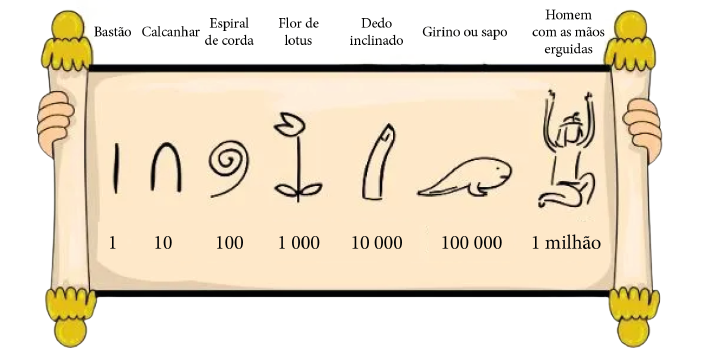
\includegraphics[width=\textwidth]{media/image2.png}\bigskip


O \textbf{sistema de numeração maia} representava os
números com pontos e traços.\bigskip

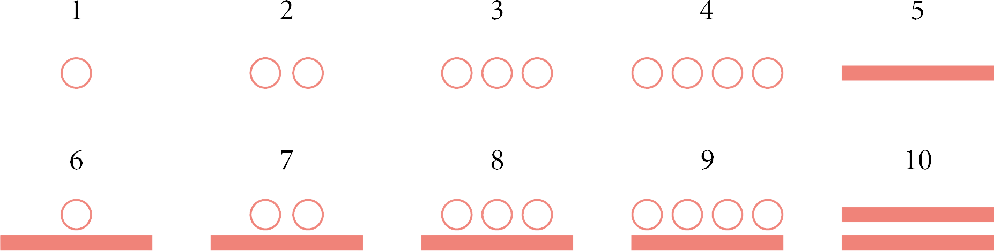
\includegraphics[width=\textwidth]{media/image3.png}\bigskip

O \textbf{sistema de numeração romano} usava letras maiúsculas 
para representar os números.\bigskip

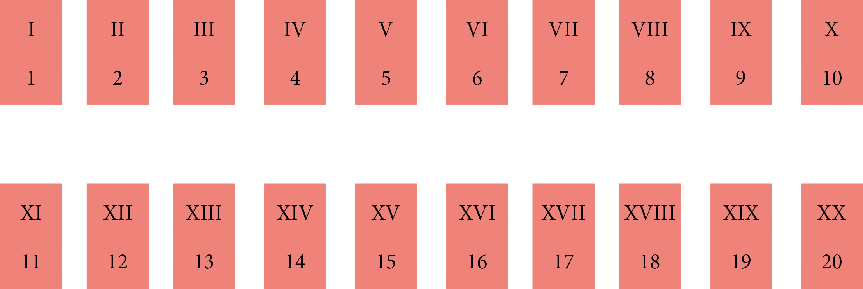
\includegraphics[width=\textwidth]{media/image4.png}\bigskip

O \textbf{sistema de numeração indo-arábico} é o sistema utilizado hoje. 
Ele passou por transformações até a atingir a forma atual.\bigskip

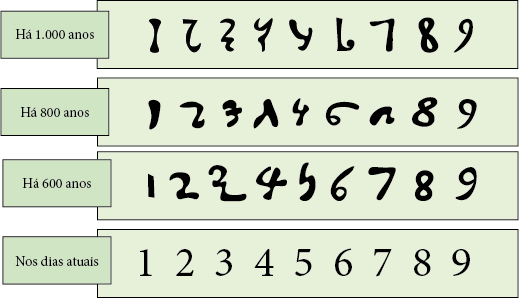
\includegraphics[width=.8\textwidth]{media/image5.png}\bigskip

No \textbf{sistema numérico indo-arábico}, os números são representados por 
pelos símbolos de 1 a 9, além do 0. Assim, em um número composto de mais
de um algarismo, ele assumo o valor posicional ou relativo, isto é, recebe 
o valor conforme a ordem e a classe. 

Por exemplo, no número 352.146, o algarismo 5 apresenta valor posicional ou
relativo igual a 50.000, pois ocupa a 5º ordem, na classe dos milhares; 
ou seja, está na posição da dezena de milhar e, sendo assim, 5 x 10.000 = 50.000.

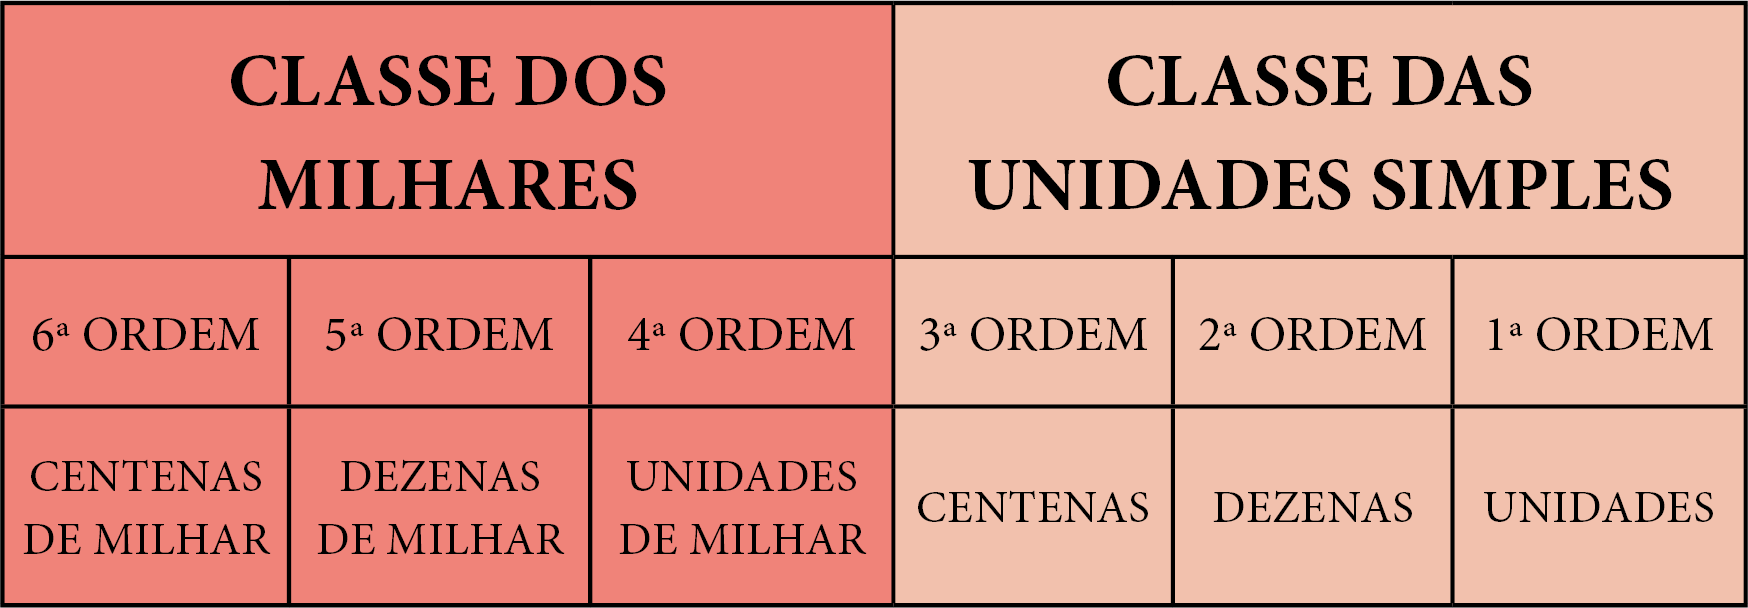
\includegraphics[width=\textwidth]{media/image1.png}\bigskip
}

\section*{Atividades}

\num{1} Escreva o valor posicional de cada algarismo
destacado, ou seja, o valor de acordo com a posição
que o algarismo ocupa no número.

\begin{escolha}
\item \textbf{8}24.345: \reduline{Valor posicional do 8 neste caso: 800.000 -- centena de milhar.\hfill}

\item 3\textbf{7}5.6\textbf{7}8: \reduline{Valor posicional da primeira ocorrência do 7 nesse caso: 70.000 -- dezena de milhar. Valor posicional da segunda ocorrência do 7 nesse caso: 70 -- dezena comum.\hfill}

\item 14\textbf{8}.52\textbf{1}:
  \reduline{Valor posicional do 8 nesse caso: 8.000 -- unidade de milhar.\hfill}
  \reduline{Valor posicional do 1 nesse caso: 1 -- unidade comum.\hfill}
\end{escolha}

\num{2} Ligue um número da coluna da esquerda com a forma escrita correspondente na coluna da direita.

\begin{figure}[htpb!]
\centering
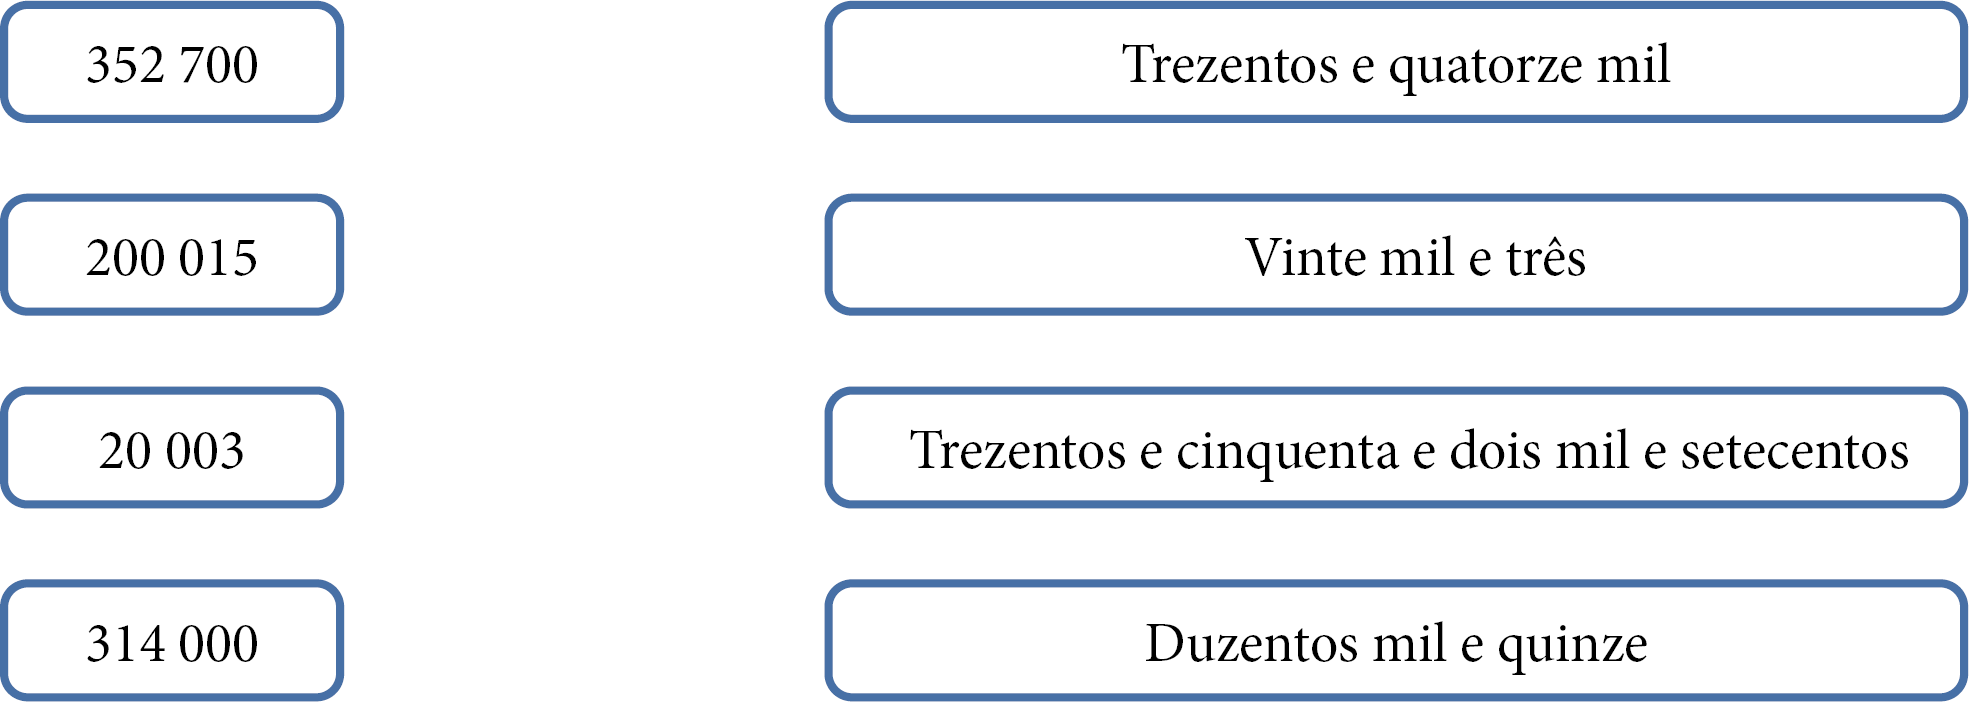
\includegraphics[width=\textwidth]{media/image6.png}
\end{figure}

\coment{352.700 deve estar ligado a trezentos e cinquenta e dois mil e setecentos; 200.015, a duzentos mil e quinze; 20.003, a vinte mil e três; 314.000, a trezentos e quatorze mil.}


\num{3} Decomponha os números a seguir de acordo com o valor posicional de cada
algarismo.

\begin{escolha}
\item 32.084
\reduline{30 000 + 2 000 + 80 + 4; 3 x 10 000 + 2 x 1 000 + 0 x 100 + 8 x 10 + 4.\hfill}

\item
  26.587
\reduline{20 000 + 6 000 + 500 + 80 + 7; 2 x 10 000 + 6 x 1 000 + 5 x 100 + 8 x 10 + 7.\hfill}
  
\item
  2.105
\reduline{2 000 + 100 + 5; 2 x 1 000 + 1 x 100 + 0 x 10 + 5.\hfill}
\end{escolha}


\num{4} Monte os número compostos e registre-os a seguir.

\begin{escolha}
\item
  7 unidades de milhar, 5 centenas e 4 unidades: \reduline{7.504.\hfill}

\item
  3 dezenas de milhar, 7 dezenas e 2 unidades: \reduline{30.072.\hfill}

\item
  9 centenas de milhar, 5 unidades de milhar e 6 centenas: \reduline{905.600.\hfill}

\item
  2 unidades de milhar, 6 centenas e 3 unidades: \reduline{2.603\hfill}
\end{escolha}

%\coment{É necessário explorar bem a montagem dos números, pois muitos alunos sabem fazer a decomposição, mas não compreendem a volta.}

\num{5} Monte um número a partir de cada composição.

\begin{escolha}
\item 5 x 100 + 4 x 10 + 5 x 1: \reduline{545.\hfill}

\item 3 x 1.000 + 0 x 100 + 9 x 10 + 3 x 1: \reduline{3.093.\hfill}

\item 4 x 10.000 + 8 x 1.000 + 5 x 100 + 0 x 10 + 2 x 1: \reduline{48.502.\hfill}

\item 3 x 100.000 + 1 x 10.000 + 6 x 1.000 + 2 x 100 + 1 x 10 + 3 x 1: \reduline{316.213.\hfill}
\end{escolha}

\num{6} Escreva por extenso cada um dos números montados na atividade anterior.

\begin{escolha}
\item \reduline{Quinhentos e quarenta e cinco.\hfill}

\item \reduline{Três mil e noventa e três.\hfill}

\item \reduline{Quarenta e oito mil quinhentos e dois.\hfill}

\item \reduline{Trezentos e dezesseis mil duzentos e treze.\hfill}
\end{escolha}

\pagebreak
\num{7} Observe os números no quadro a seguir e relacione cada um a uma característica.

\begin{mdframed}[linewidth=2pt,linecolor=azul!20,backgroundcolor=azul!20,roundcorner=2pt]
\textbf{147.254 \hfill 464.823 \hfill 9.998 \hfill 99.999}
\end{mdframed}

\begin{escolha}
\item O maior número com exatamente 5 ordens. \reduline{99.999.\hfill}

\item O segundo maior número formado por 4 ordens. \reduline{9.998.\hfill}

\item Um número ímpar com 6 ordens. \reduline{464 823.\hfill}

\item Um número de 6 ordens com algarismo da unidade de milhar igual a 7. \reduline{147.254.\hfill}
\end{escolha}

\num{8} Represente os números a seguir utilizando os símbolos maias.

\begin{escolha}
\item   11
\reduline{O aluno deve usar duas linhas e um ponto.\hfill}

\item  12
\reduline{O aluno deve usar duas linhas e dois pontos.\hfill}


\item  13
\reduline{O aluno deve usar duas linhas e três pontos.\hfill}

\item  14
\reduline{O aluno deve usar duas linhas e quatro pontos.\hfill}

\item  15
\reduline{O aluno deve usar duas linhas seguidas de uma linha.\hfill}

\item  16
\reduline{O aluno deve usar duas linhas seguidas de um ponto sobre uma linha.\hfill}

\item  17
\reduline{O aluno deve usar duas linhas seguidas de dois pontos sobre uma linha.\hfill}

\item  18
\reduline{O aluno deve usar duas linhas seguidas de três pontos sobre uma linha.\hfill}

\item  19
\reduline{O aluno deve usar duas linhas seguidas de quatro pontos sobre uma linha.\hfill}
\end{escolha}

\num{9} Escreva cada um dos números a seguir utilizando o sistema indo-arábico.

\begin{escolha}
\item
  Dois mil trezentos e cinco: \reduline{2.305\hfill}
\item
  Quinze mil e quarenta e sete: \reduline{15.047\hfill}
\item
  Vinte mil e novecentos: \reduline{20.900\hfill}
\item
  Trinta e três mil trezentos e trinta e três: \reduline{33.333\hfill}
\item
  Cinquenta mil e cinco: \reduline{50.005\hfill}
\end{escolha}

\begin{comment}
\num{10} A bolas representadas a seguir fazem parte de um jogo conhecido como
bilhar ou como sinuca.

\begin{figure}[htpb!]
\centering
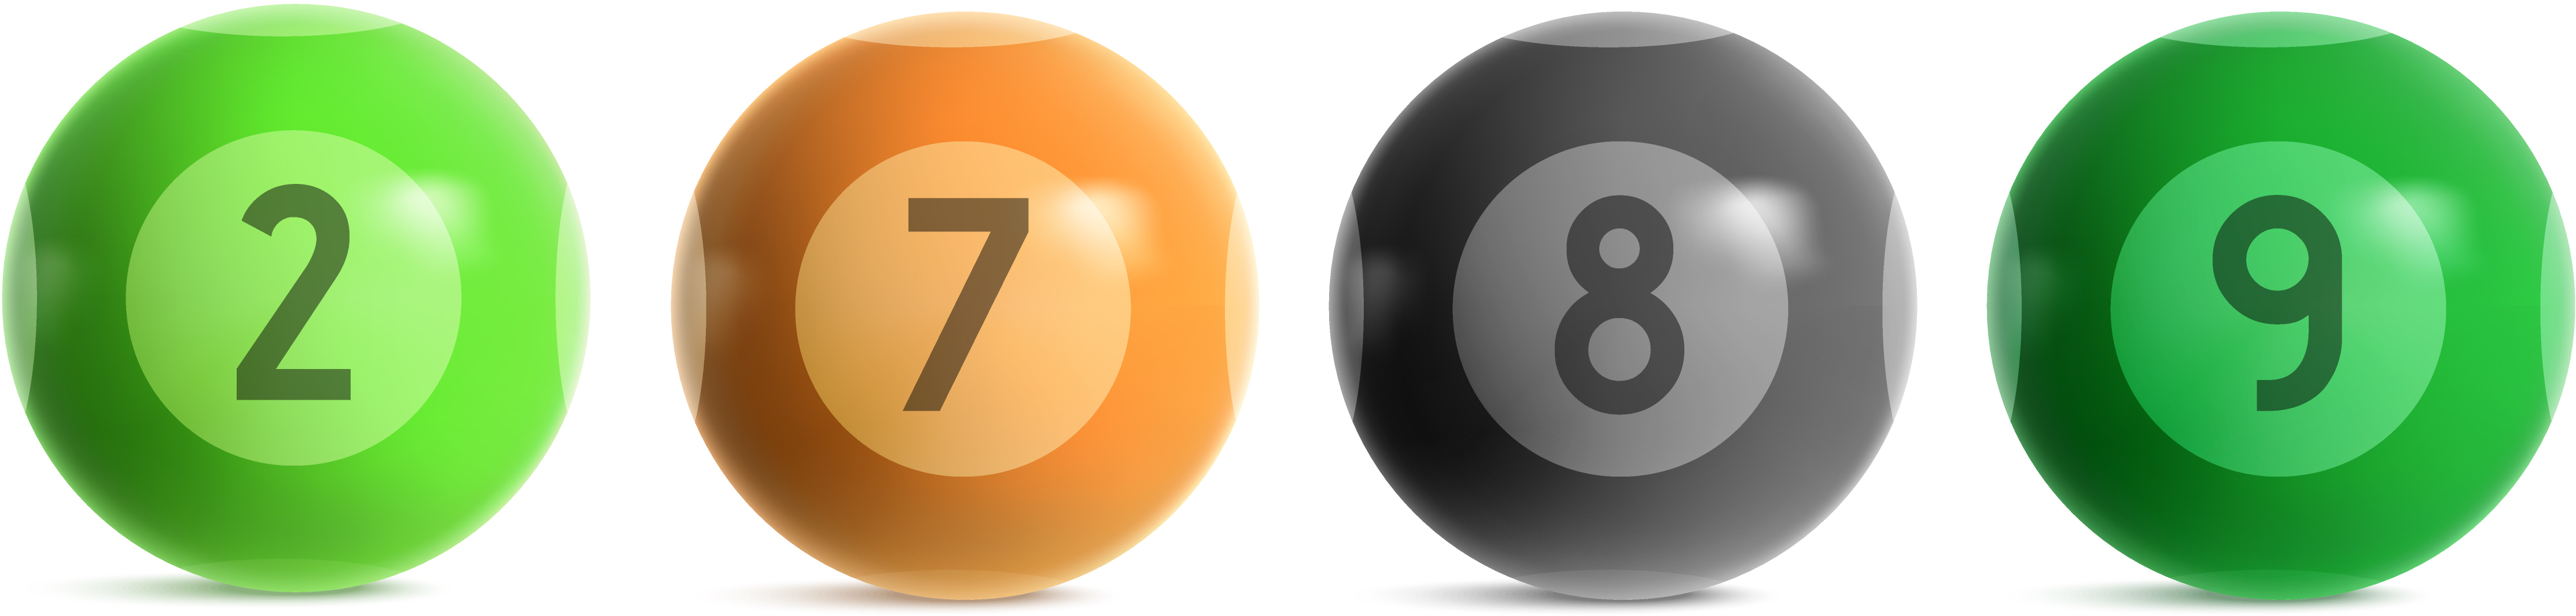
\includegraphics[width=\textwidth]{media/image7.png}
\end{figure}


Observando os números representados em cada bola, responda ao que se pergunta a seguir.

\begin{escolha}
\item
  Qual é o menor número entre essas bolas? \reduline{2 (dois).\hfill}

\item
  Qual é o menor número com exatamente 4 ordens que podemos formar com essas bolas? \reduline{2.789 (dois mil setecentos e oitenta e nove).\hfill}

\item
  Qual é o maior número par que podemos formar com essas bolas? \reduline{9.872 (nove mil oitocentos e setenta e dois).\hfill}
\end{escolha}

%Explore mais exemplos com os alunos para estimular a formação de números e a criatividade de cada um deles.
\end{comment}

\num{10} Observe o relógio na imagem e escreva, por extenso, que horas são.

\begin{center}
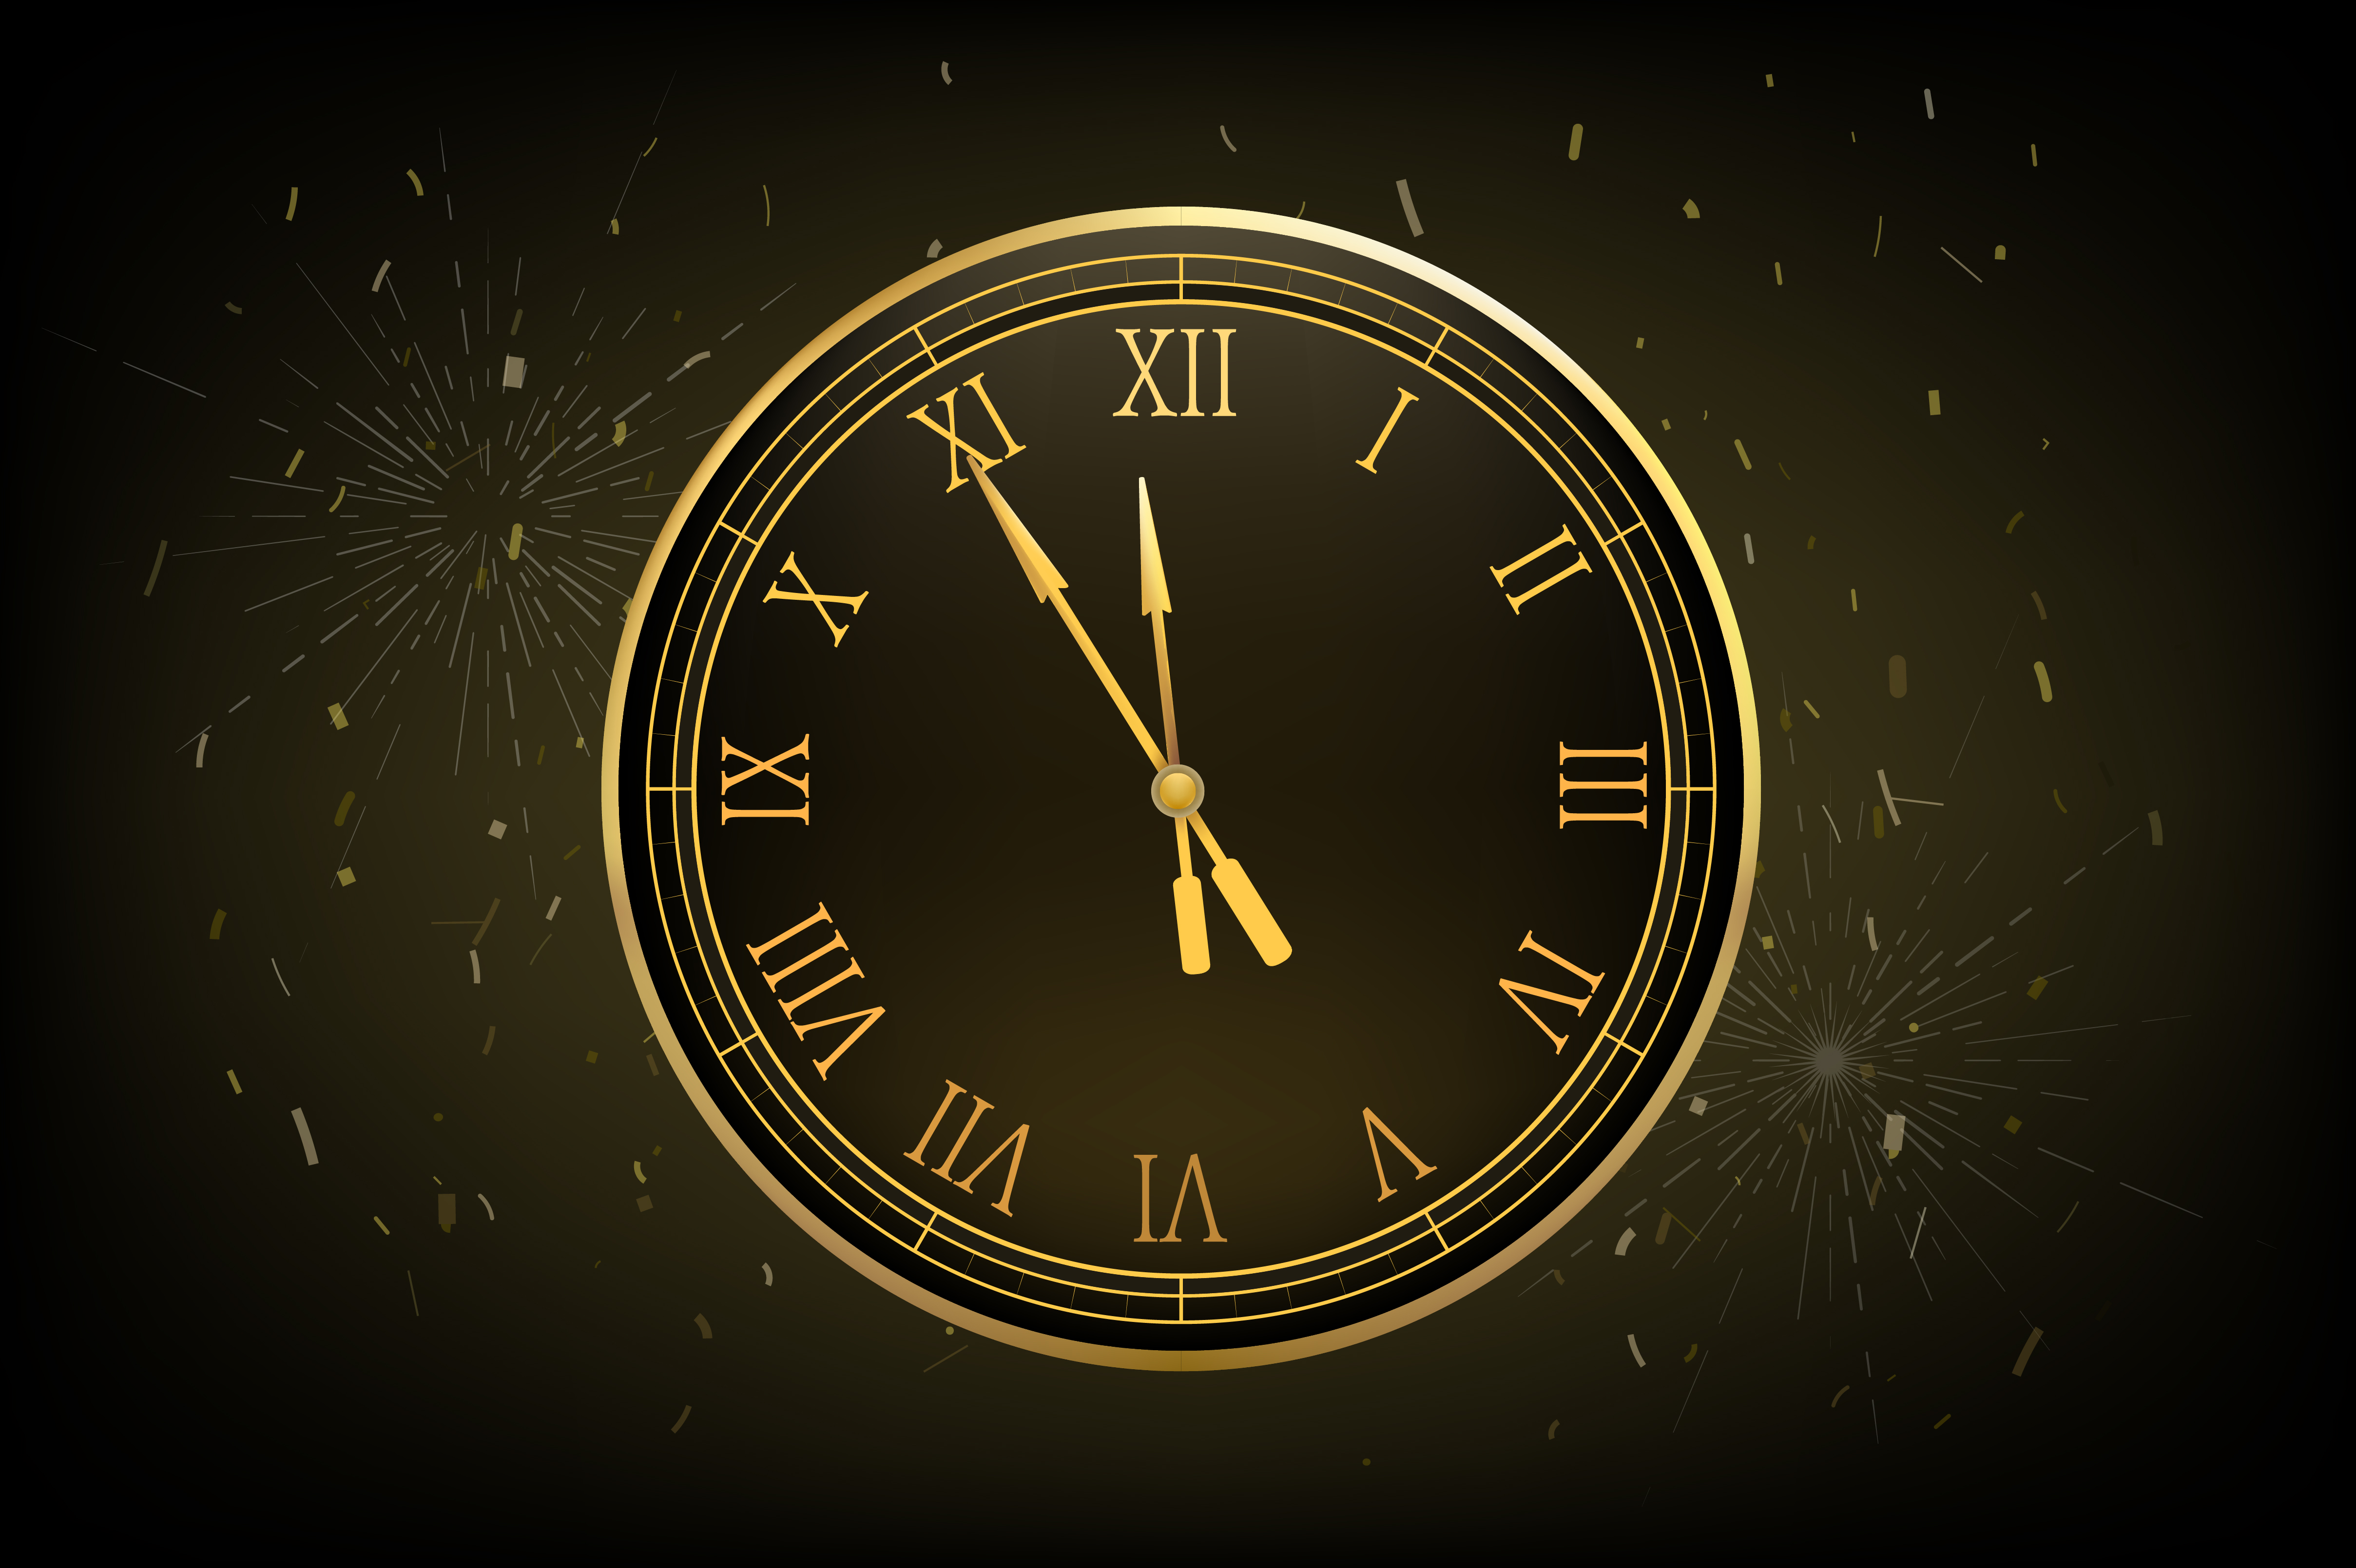
\includegraphics[width=.8\textwidth]{media/image7a.jpeg}
\end{center}

\reduline{No mostrador do relógio da imagem, são onze horas e ciquenta e cinco minutos.\hfill}
\linhas{1}

\pagebreak
\section*{Treino}

\num{1} Amanda estava brincando na praça quando olhou para uma casa nas proximidades e viu um
o número 2.342:

\begin{figure}[htpb!]
\centering
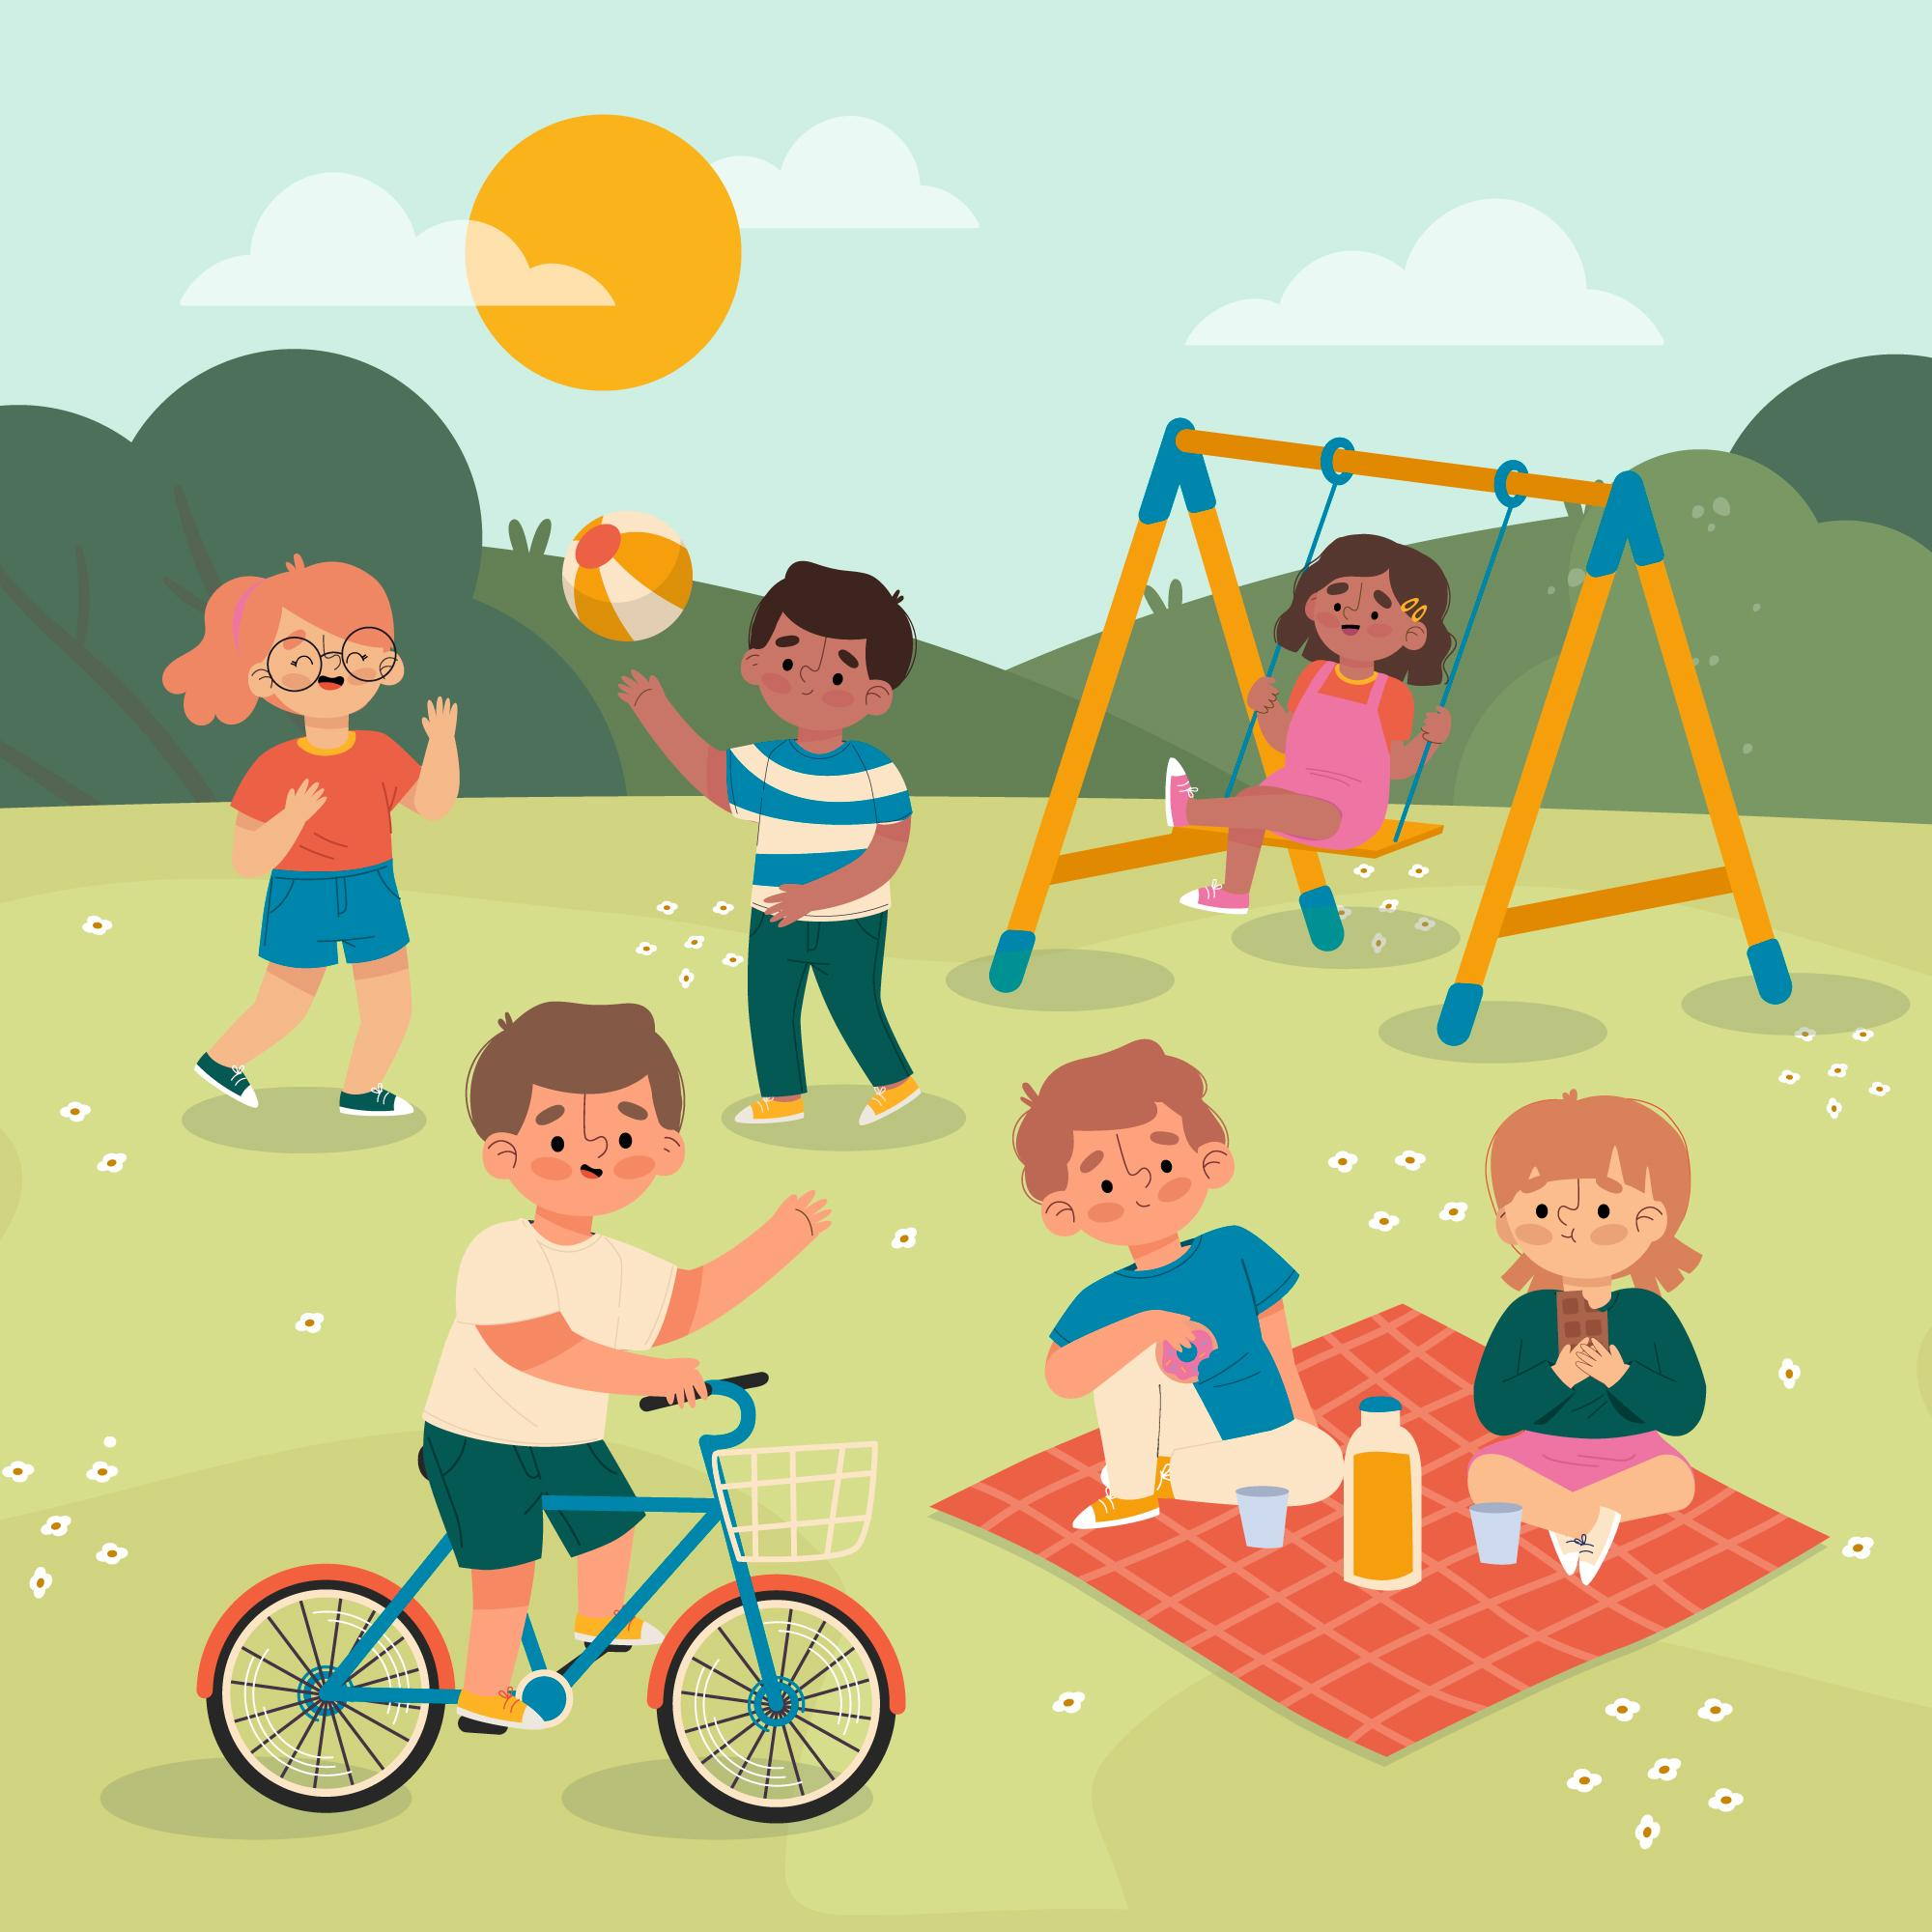
\includegraphics[width=\textwidth]{media/image8a.jpeg}
\end{figure}

Lembrando-se das aulas de Matemática, a menina resolveu decompor o número escrito
no papel. Qual é a decomposição correta que Amanda poderá fazer desse
número?

\begin{multicols}{2}
\begin{escolha}
\item
  2.000 + 300 + 40 + 2.
\item
  2.000 + 400 + 40 + 2.
\item
  2.000 + 300 + 20 + 2.
\item
  2.000 + 200 + 40 + 1.
\end{escolha}
\end{multicols}

\pagebreak
\num{2} Vitor escreveu o seguinte número utilizando os algarismos romanos:

\conteudo{
\begin{center}
\textbf{XIX}
\end{center}
}

Esse número, no sistema indo-arábico, é o:

\begin{escolha}
\item
  9.
\item
  19.
\item
  21.
\item
  11.
\end{escolha}

\num{3} Antônio encontrou um papel no chão da escola a seguinte decomposição.  

\begin{figure}[htpb!]
\centering
\includegraphics[width=\textwidth]{media/image8b.jpeg}
\end{figure} 

O número decomposto é:

\begin{escolha}
\item 341.963.

\item 347.963.

\item 340.963.

\item 347.962.

\end{escolha} 


\begin{comment}
\pagebreak
\num{3} José resolveu comprar uma placa com o número de sua casa. Observe a seguir.

\begin{figure}[htpb!]
\centering
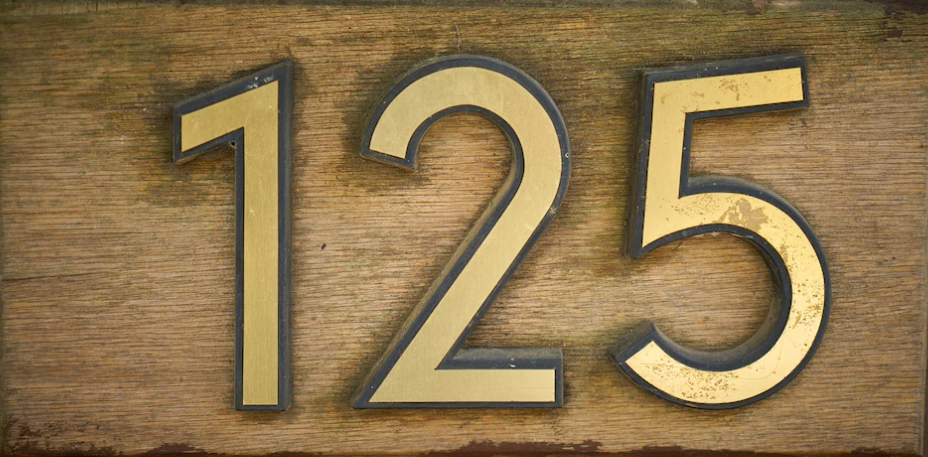
\includegraphics[width=.5\textwidth]{media/image9.png}
\end{figure}

Depois, percebeu que o número estava
errado, já que o primeiro e o último algarismo estão nas posições
trocadas. Qual é o valor relativo do último algarismo no lugar em que ele se
encontra na placa errada e qual deveria ser seu valor relativo no número
correto da casa de José?

\begin{escolha}
\item
  Está como 5 e deveria ser como 50.
\item
  Está como 50 e deveria ser como 500.
\item
  Está como 5 e deveria ser como 500.
\item
  Está como 50 e deveria ser como 5.
\end{escolha}
\end{comment}


\chapter{As operações básicas}
\markboth{Módulo 2}{}

\section*{Habilidades do SAEB}

\begin{itemize}
\item Calcular o resultado de adições ou subtrações envolvendo números
naturais de até 6 ordens.
\item Calcular o resultado de multiplicações ou divisões envolvendo números
naturais de até 6 ordens.
\item Associar o quociente de uma divisão com resto zero de um número
natural de até 6 ordens por 2, 3, 4, 5 e 10 às ideias de metade, terça,
quarta, quinta e décima parte.
\item Resolver problemas de adição ou de subtração, envolvendo números
naturais de até 6 ordens, com os significados de juntar, acrescentar,
separar, retirar, comparar ou completar.
\item Resolver problemas de multiplicação ou de divisão, envolvendo números
naturais de até 6 ordens, com os significados de formação de grupos
iguais (incluindo repartição equitativa e medida), proporcionalidade ou
disposição retangular.
\end{itemize}

\subsection{Habilidade da BNCC}

\begin{itemize}
\item EF04MA07.
\end{itemize}

\conteudo{
\textbf{Operações matemáticas}

As operações básicas da matemática são adição, subtração, multiplicação e divisão. 
Elas são as ferramentas utilizadas para manipular números e resolver
uma variedade de problemas. Cada uma delas tem sua própria função e aplicações específicas.

\begin{itemize}
\item\textbf{Adição}
\end{itemize}

A adição combina dois ou mais números em um valor total. 
Ela é usada para calcular somas, encontrar o total de itens, 
calcular o aumento de quantidades e muito mais.\bigskip

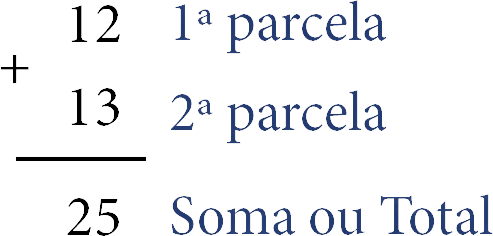
\includegraphics[width=.3\textwidth]{media/image10.png}\bigskip

\begin{itemize}
\item\textbf{Subtração}
\end{itemize}

A subtração permite encontrar a diferença entre dois números, 
determinar o troco, calcular a distância entre pontos 
e resolver problemas de redução.\bigskip

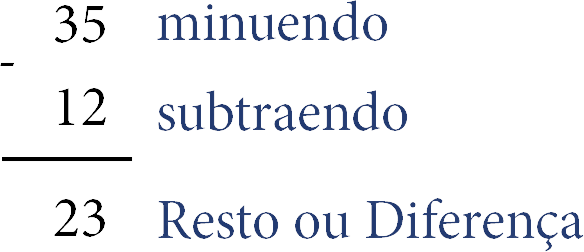
\includegraphics[width=.3\textwidth]{media/image11.png}\bigskip

\begin{itemize}
\item\textbf{Multiplicação}
\end{itemize}

A multiplicação é a operação que repete uma mesma quantidade várias vezes. 
Assim, se houver 3 caixas com 4 lápis cada caixa e for necessário determinar 
quantos lápis há no total. Multiplica-se 3 vezes 4, para obter o resultado de 12 lápis.\bigskip

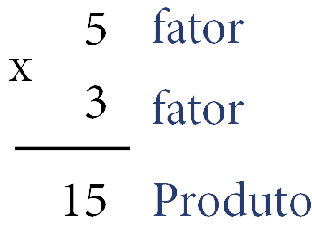
\includegraphics[width=.2\textwidth]{media/image12.png}\bigskip

\begin{itemize}
\item\textbf{Divisão}
\end{itemize}

A divisão pode ser usada, por exemplo, quando é necessário reunir coisas em grupos iguais. 
Se tivermos 12 balas e dividirmos igualmente entre 3 amigos, cada amigo ficará com 4 balas.\bigskip

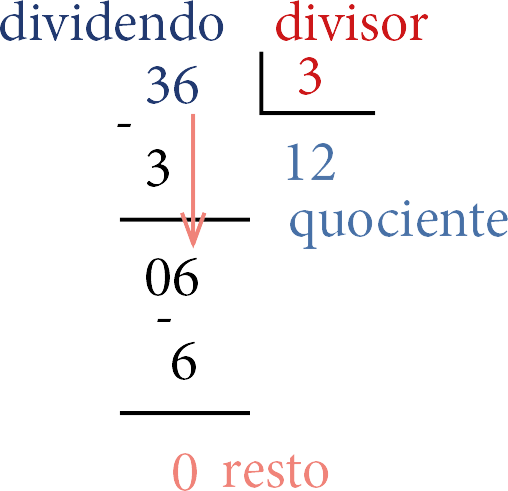
\includegraphics[width=.2\textwidth]{media/image13.png}\bigskip

Conhecer os números e as operações permite resolver problemas matemáticos 
nas situações mais comuns do cotidiano pelas quais cada um passa, 
como contar brinquedos, medir o tamanho de coisas, dividir doces com amigos e muito mais. 
É como uma linguagem especial que nos ajuda a entender o mundo ao nosso redor!
}

\section*{Atividades}

\num{1} Ligue cada operação da coluna da esquerda com o resultado correto na
coluna da direita.

\begin{figure}[htpb!]
\centering
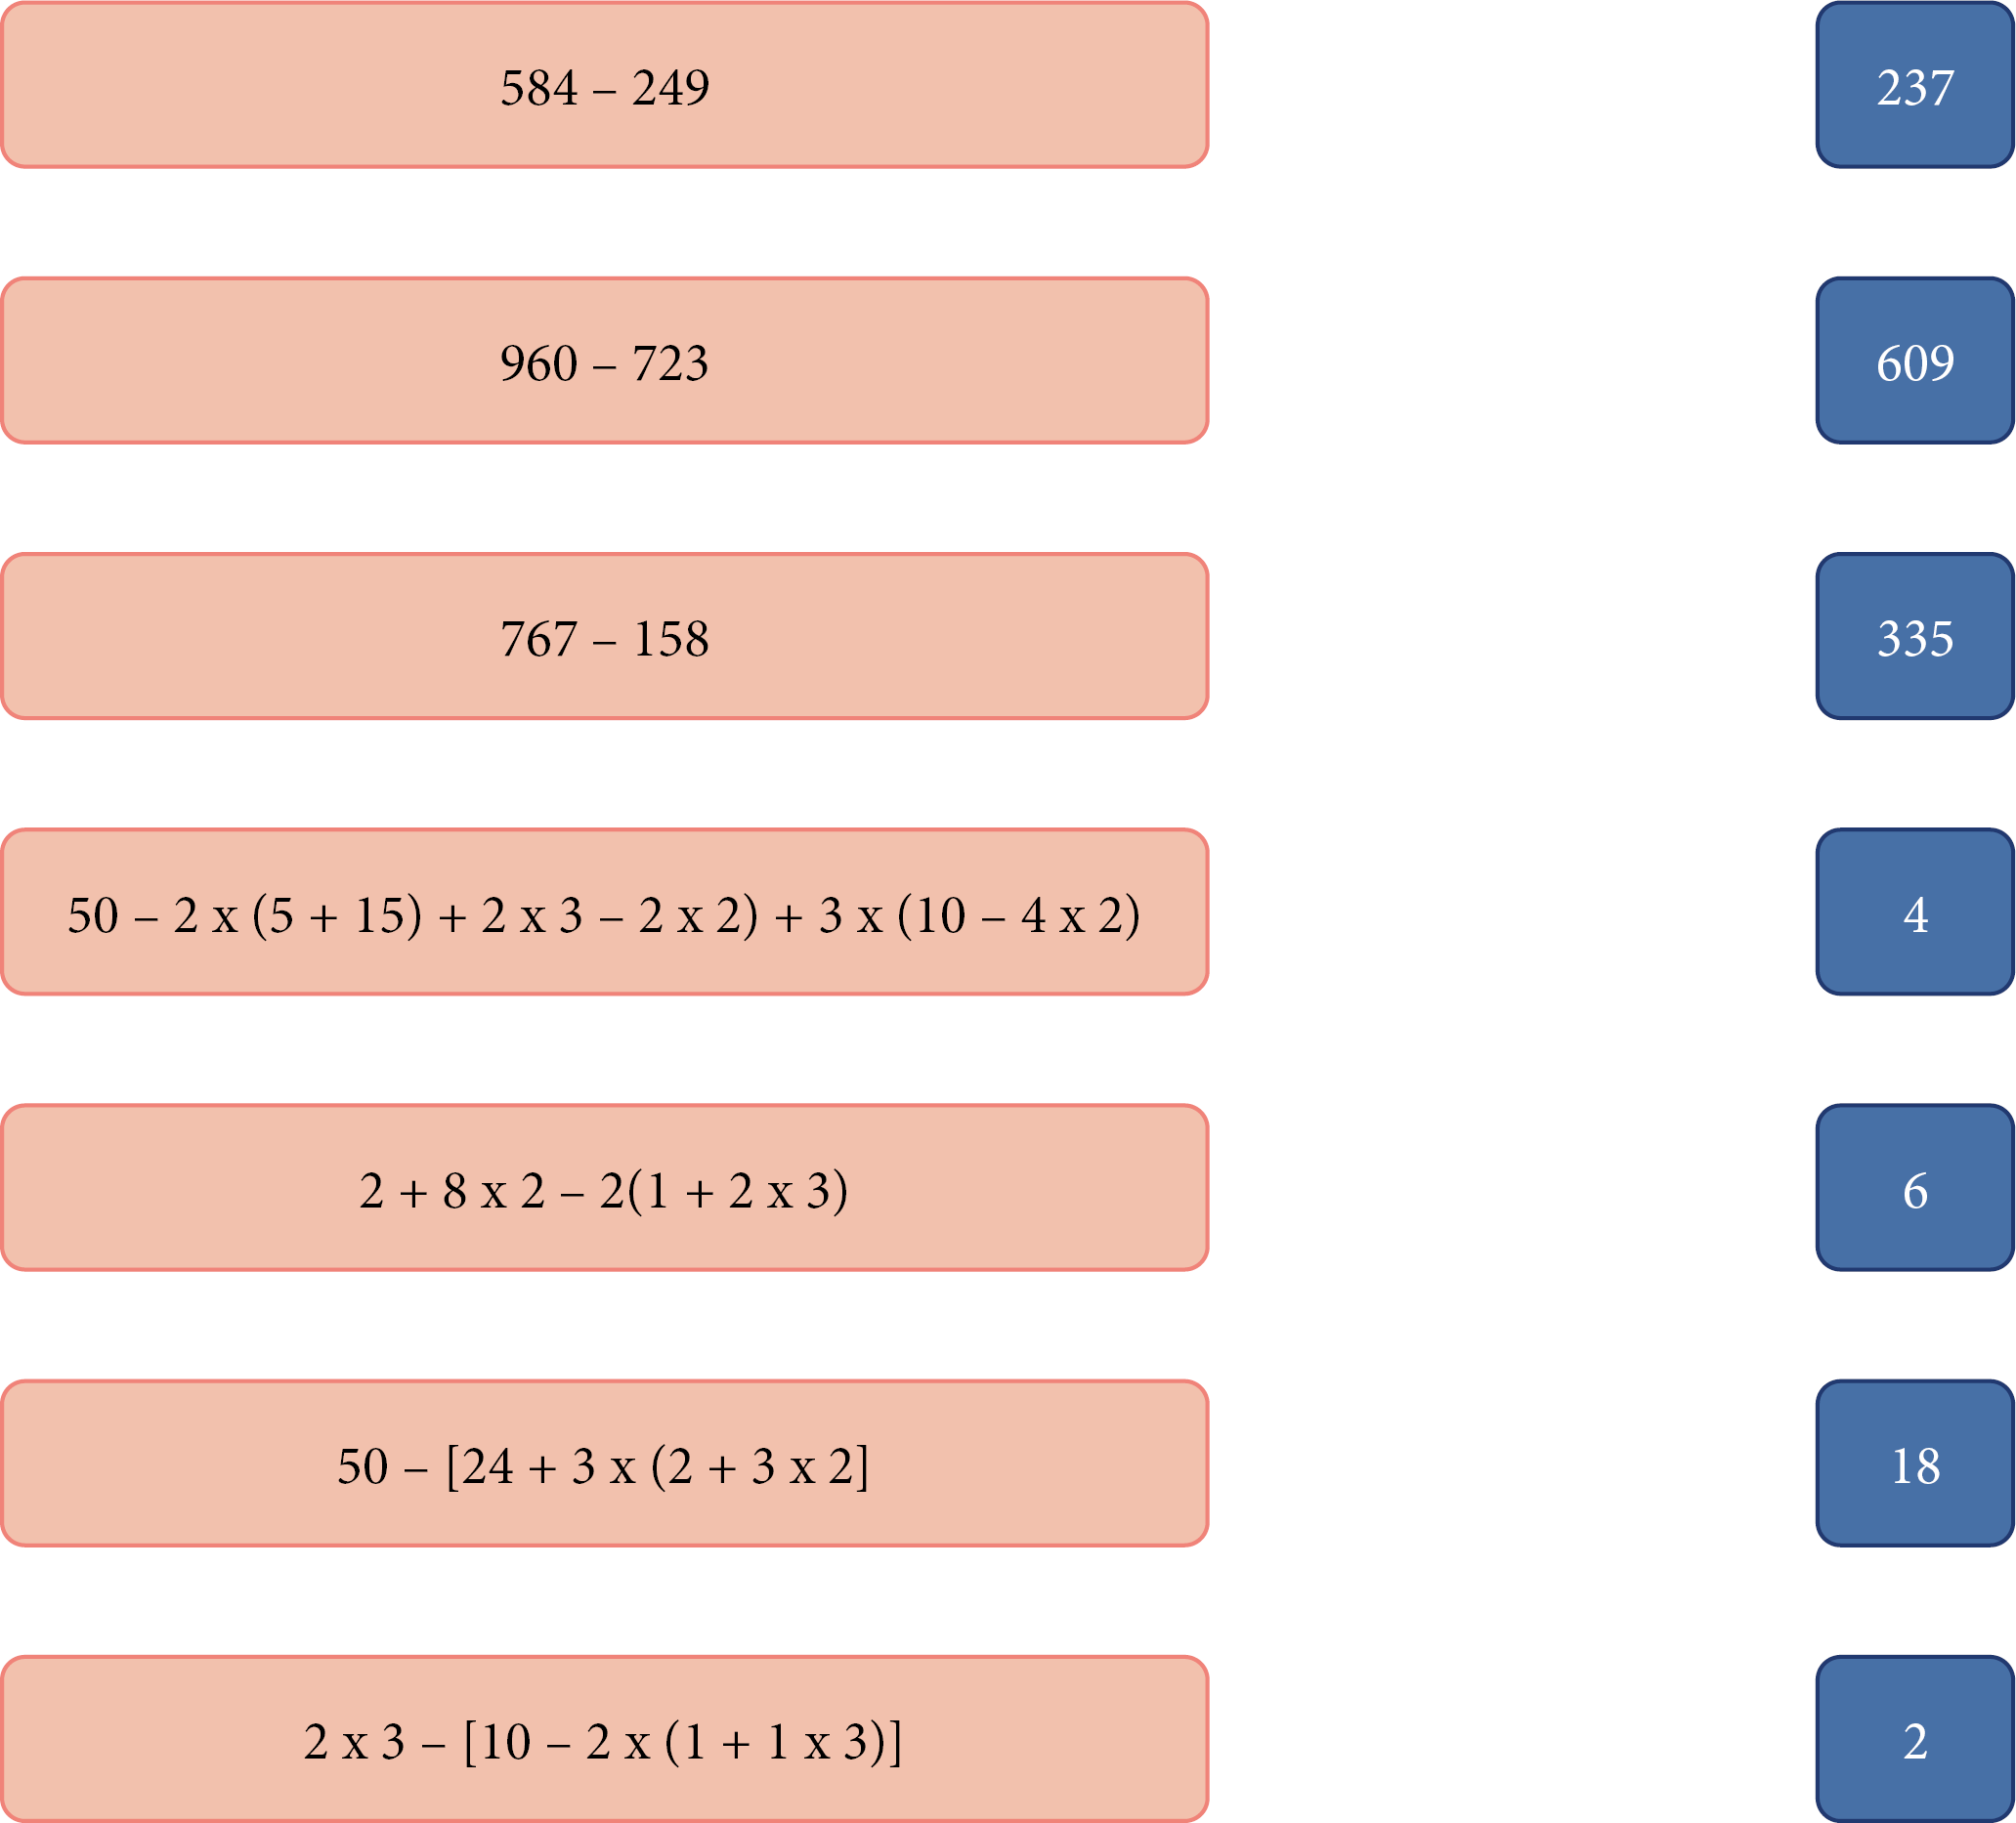
\includegraphics[width=.9\textwidth]{media/image14.png}
\end{figure}
\pagebreak


\num{2} O pai de Cláudio precisa realizar um pequeno reparo na cozinha de sua casa.
Para isso, será necessário fazer concreto, um composto de cimento, areia e água. 
Uma das possibilidades para produzi-lo é misturar uma parte de cimento, 
três partes de areia e três de água. Se ele utilizou 250 gramas de cimento, 
qual será a quantidade necessária de areia? 

\begin{figure}[htpb!]
\centering
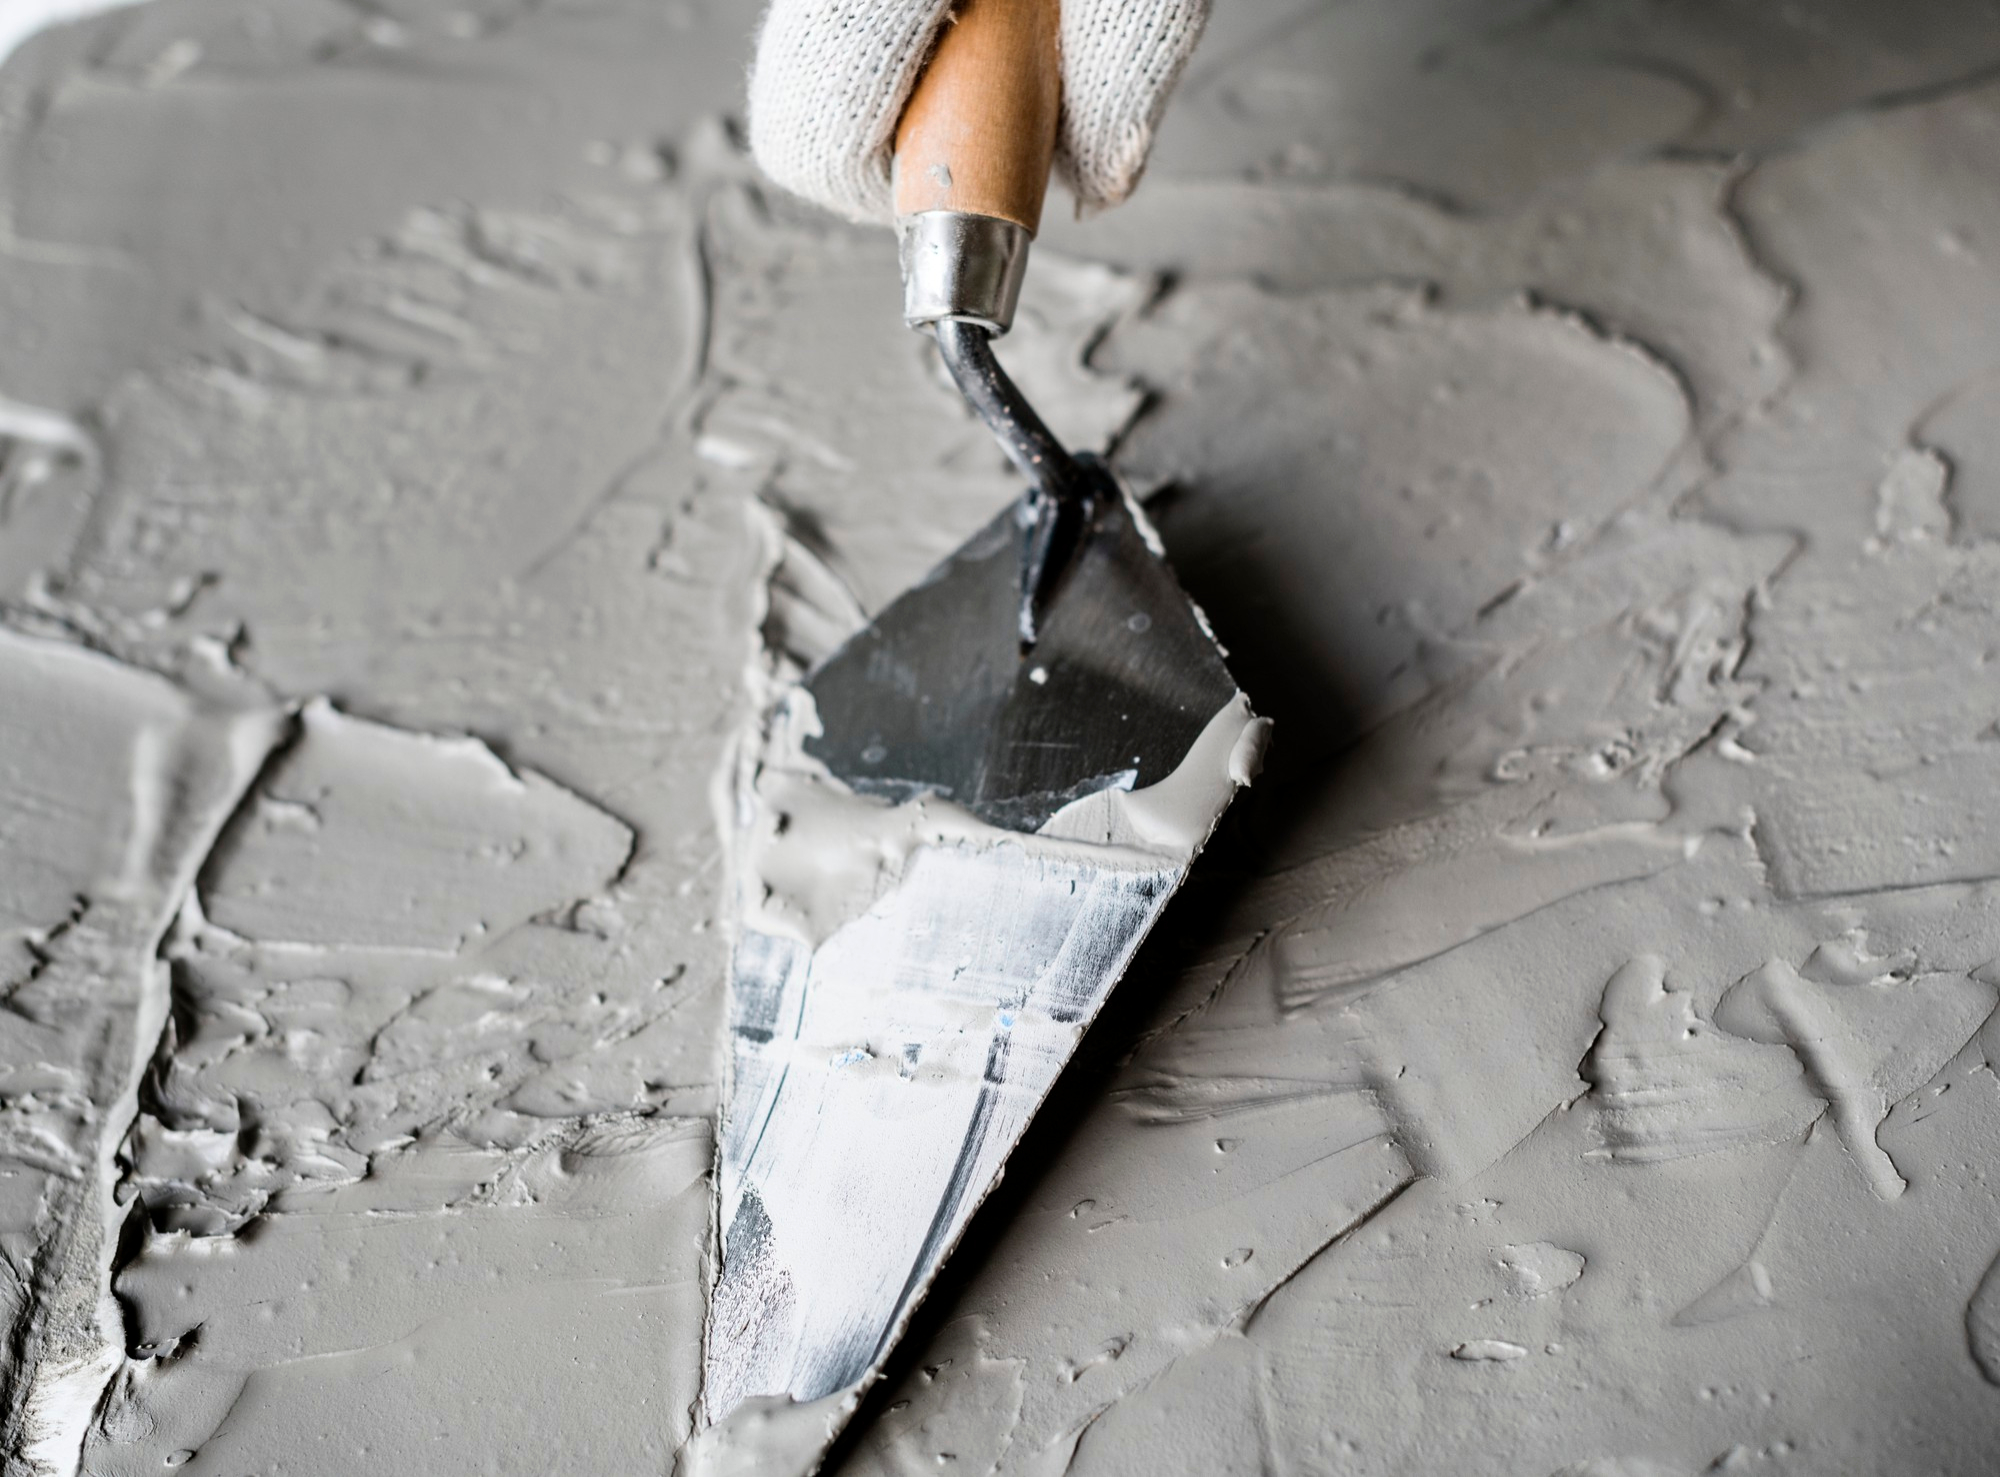
\includegraphics[width=.5\textwidth]{media/image14a.jpg}
\end{figure}

\reduline{Cládio usará 250 g de areia. Assim sendo, 250 g x 3 = 750 g de areia.\hfill}


\begin{comment}
Segundo a receita de um bolo, devem-se inicialmente colocar 260 g de farinha
de trigo e misturar com outros ingredientes como ovos, açúcar e leite.
Em seguida, devem-se colocar mais 135 g de farinha de trigo para a massa
ficar no ponto ideal. Qual é a quantidade total de farinha, em quilogramas,
utilizada nessa receita?

\reduline{260 + 135 = 395 g = 0,395 kg.\hfill}
\end{comment}


\num{3} O quadro a seguir mostra a população do Amapá dividida em municípios, segundo estimativa do IBGE de 2018.

\begin{longtable}[]{@{}ll@{}}
\toprule
Município & População estimada\tabularnewline
\midrule
\endhead
Macapá (capital) & 503.907\tabularnewline
Santana & 122.988\tabularnewline
Laranjal do Jari & 55.021\tabularnewline
Oiapoque & 29.563\tabularnewline
Mazagão & 27.436\tabularnewline
Porto Grande & 22.286\tabularnewline
Tartarugalzinho & 17.206\tabularnewline
Pedra Branca do Amapari & 16.624\tabularnewline
Vitória do Jari & 15.632\tabularnewline
Calçoene & 12.165\tabularnewline
Amapá & 10.842\tabularnewline
Ferreira Gomes & 9.373\tabularnewline
Cutias & 7.816\tabularnewline
Itaubal & 6.400\tabularnewline
Serra do Navio & 6.301\tabularnewline
Pracuuba & 5.632\tabularnewline
\bottomrule
\end{longtable}

A somatória das populações dos municípios sem contar a capital é maior ou menor que a população de Macapá? Justifique sua resposta com cálculos.

\reduline{122.988 + 55.021 + 29.563 + 27.436 + 22.286 + 17.206 + 16.624 + 15.632 + 12.165 + 10.842 + 9.373 + 7.816 + 6.400 + 6.301 + 5.632 = 365.285 (menor que a população da capital, que é de 503.907).\hfill}

%\coment{Portanto a soma das populações estimadas dos municípios apresentados na
%tabela, exceto São Paulo, é menor que a população da cidade de São
%Paulo.}

\num{4} Faça o que se pede a seguir.

\begin{figure}[htpb!]
\centering
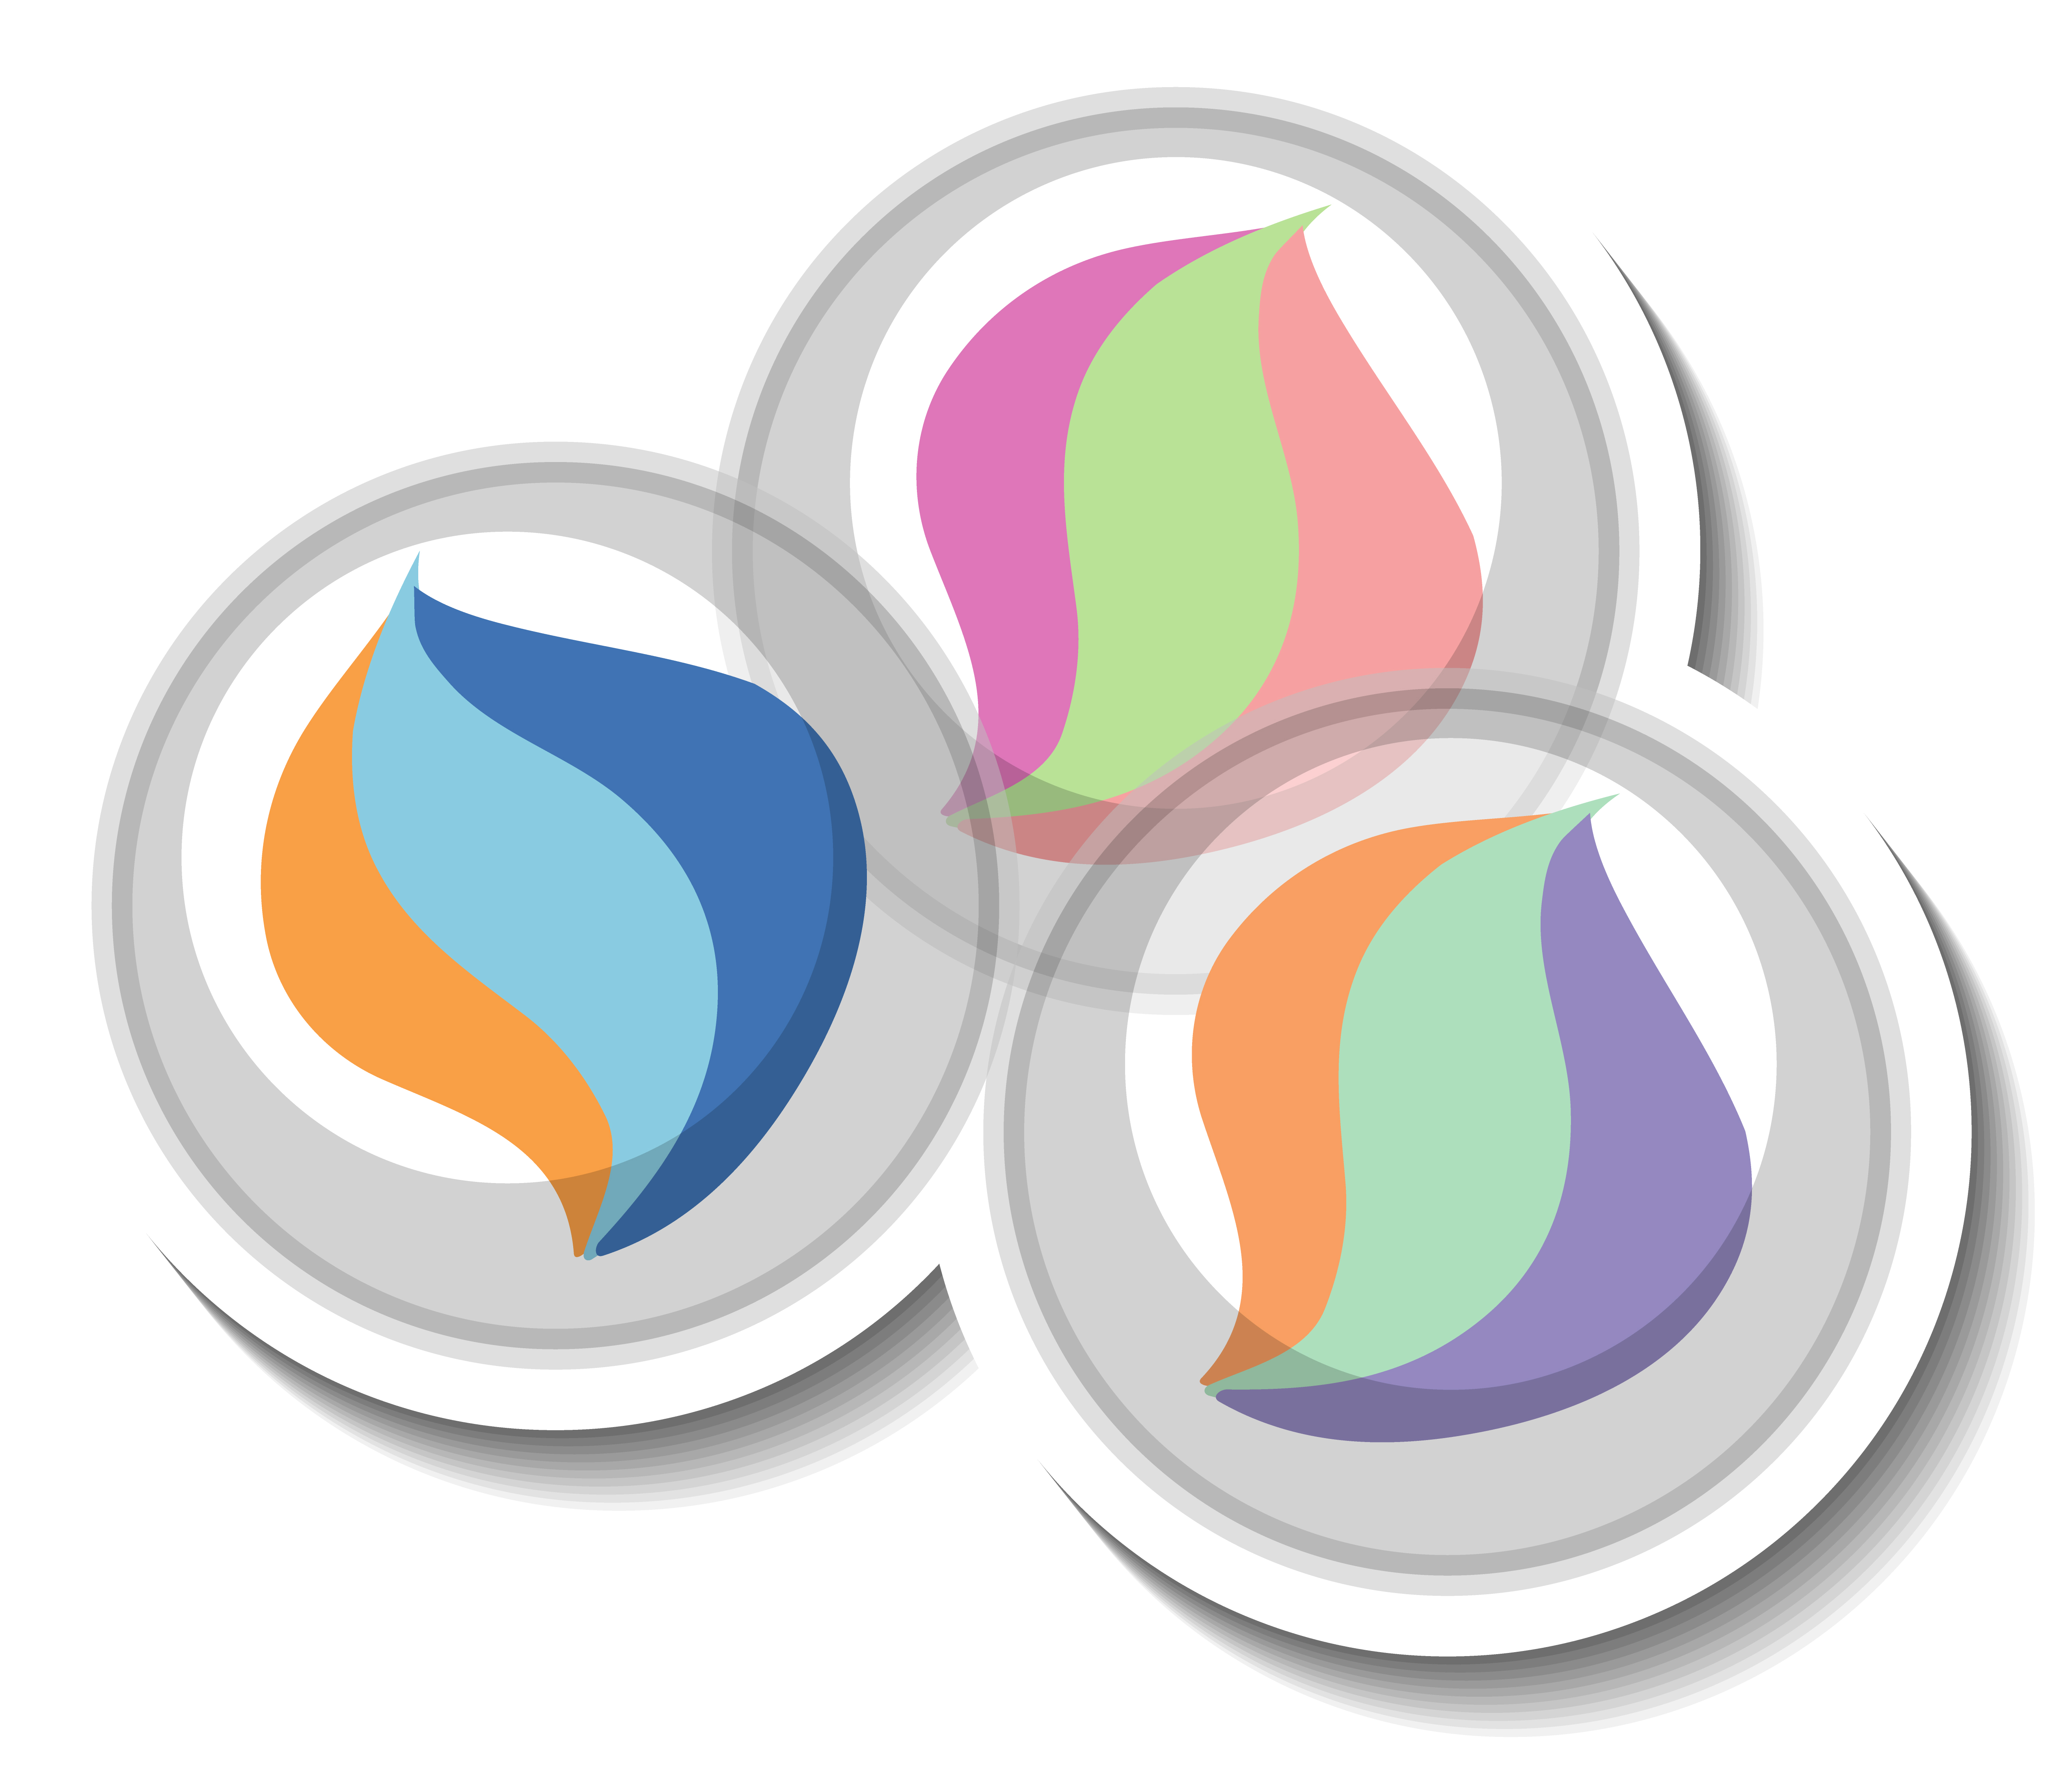
\includegraphics[width=.5\textwidth]{media/image14b.jpeg}
\end{figure}

\begin{escolha}
\item
  Se em uma caixa cabem 1.000 bolinhas de gude de mesmo tamanho, quantas
  caixas precisaremos para guardar 6.536 bolinhas de gude desse mesmo
  tamanho?
\reduline{6.536 : 1.000 = 6 + 536 de resto; portanto serão necessárias 7 caixas
    (6 caixas completas e 1 com 536 bolinhas apenas).\hfill}

\item
  Se na caixa couberem apenas 100 bolinhas de gude de mesmo tamanho, quantas
  caixas serão necessárias para armazenar essas mesmas 6.536 bolinhas?
\reduline{6.536 : 100 = 65 + 36 de resto; portanto serão necessárias 66 caixas
    (65 caixas completas e 1 com 36 bolinhas apenas).\hfill}

\item
  Se a caixa só puder armazenar 10 bolinhas de mesmo tamanho, quantas caixas dessas
  serão necessárias para armazenar as mesmas 6.536 bolinhas de gude?
\reduline{6.536 : 10 = 653 + 6 de resto; portanto serão necessárias 654 caixas
    (653 caixas completas e 1 com 6 bolinhas apenas).\hfill}
\end{escolha}

\num{5} Faça o que se pede a seguir.

\begin{escolha}
\item Uma coleção de álbuns de figurinhas conta com cinco volumes temáticos: animais da savana, animais da Ásia, animais da Austrália, animais do Ártico e animais das Américas. Em cada volume, o colecionador precisa de 45 figurinhas para completar o álbum. Calcule quantas figurinhas são necessárias para completar a coleção toda.
\reduline{São necessárias 45 figurinhase em cada volume, e são 5 volumes. Logo: 5 x 45 = 225 figurinhas para a coleção toda.\hfill}

\item Uma grande exposição de obras de arte de vários artistas está dividida em 108 seções, e em cada seção há entre 6 e 9 obras de arte. Calcule o número mínimo e o número máximo de obras que pode haver na exposição toda?

\begin{center}
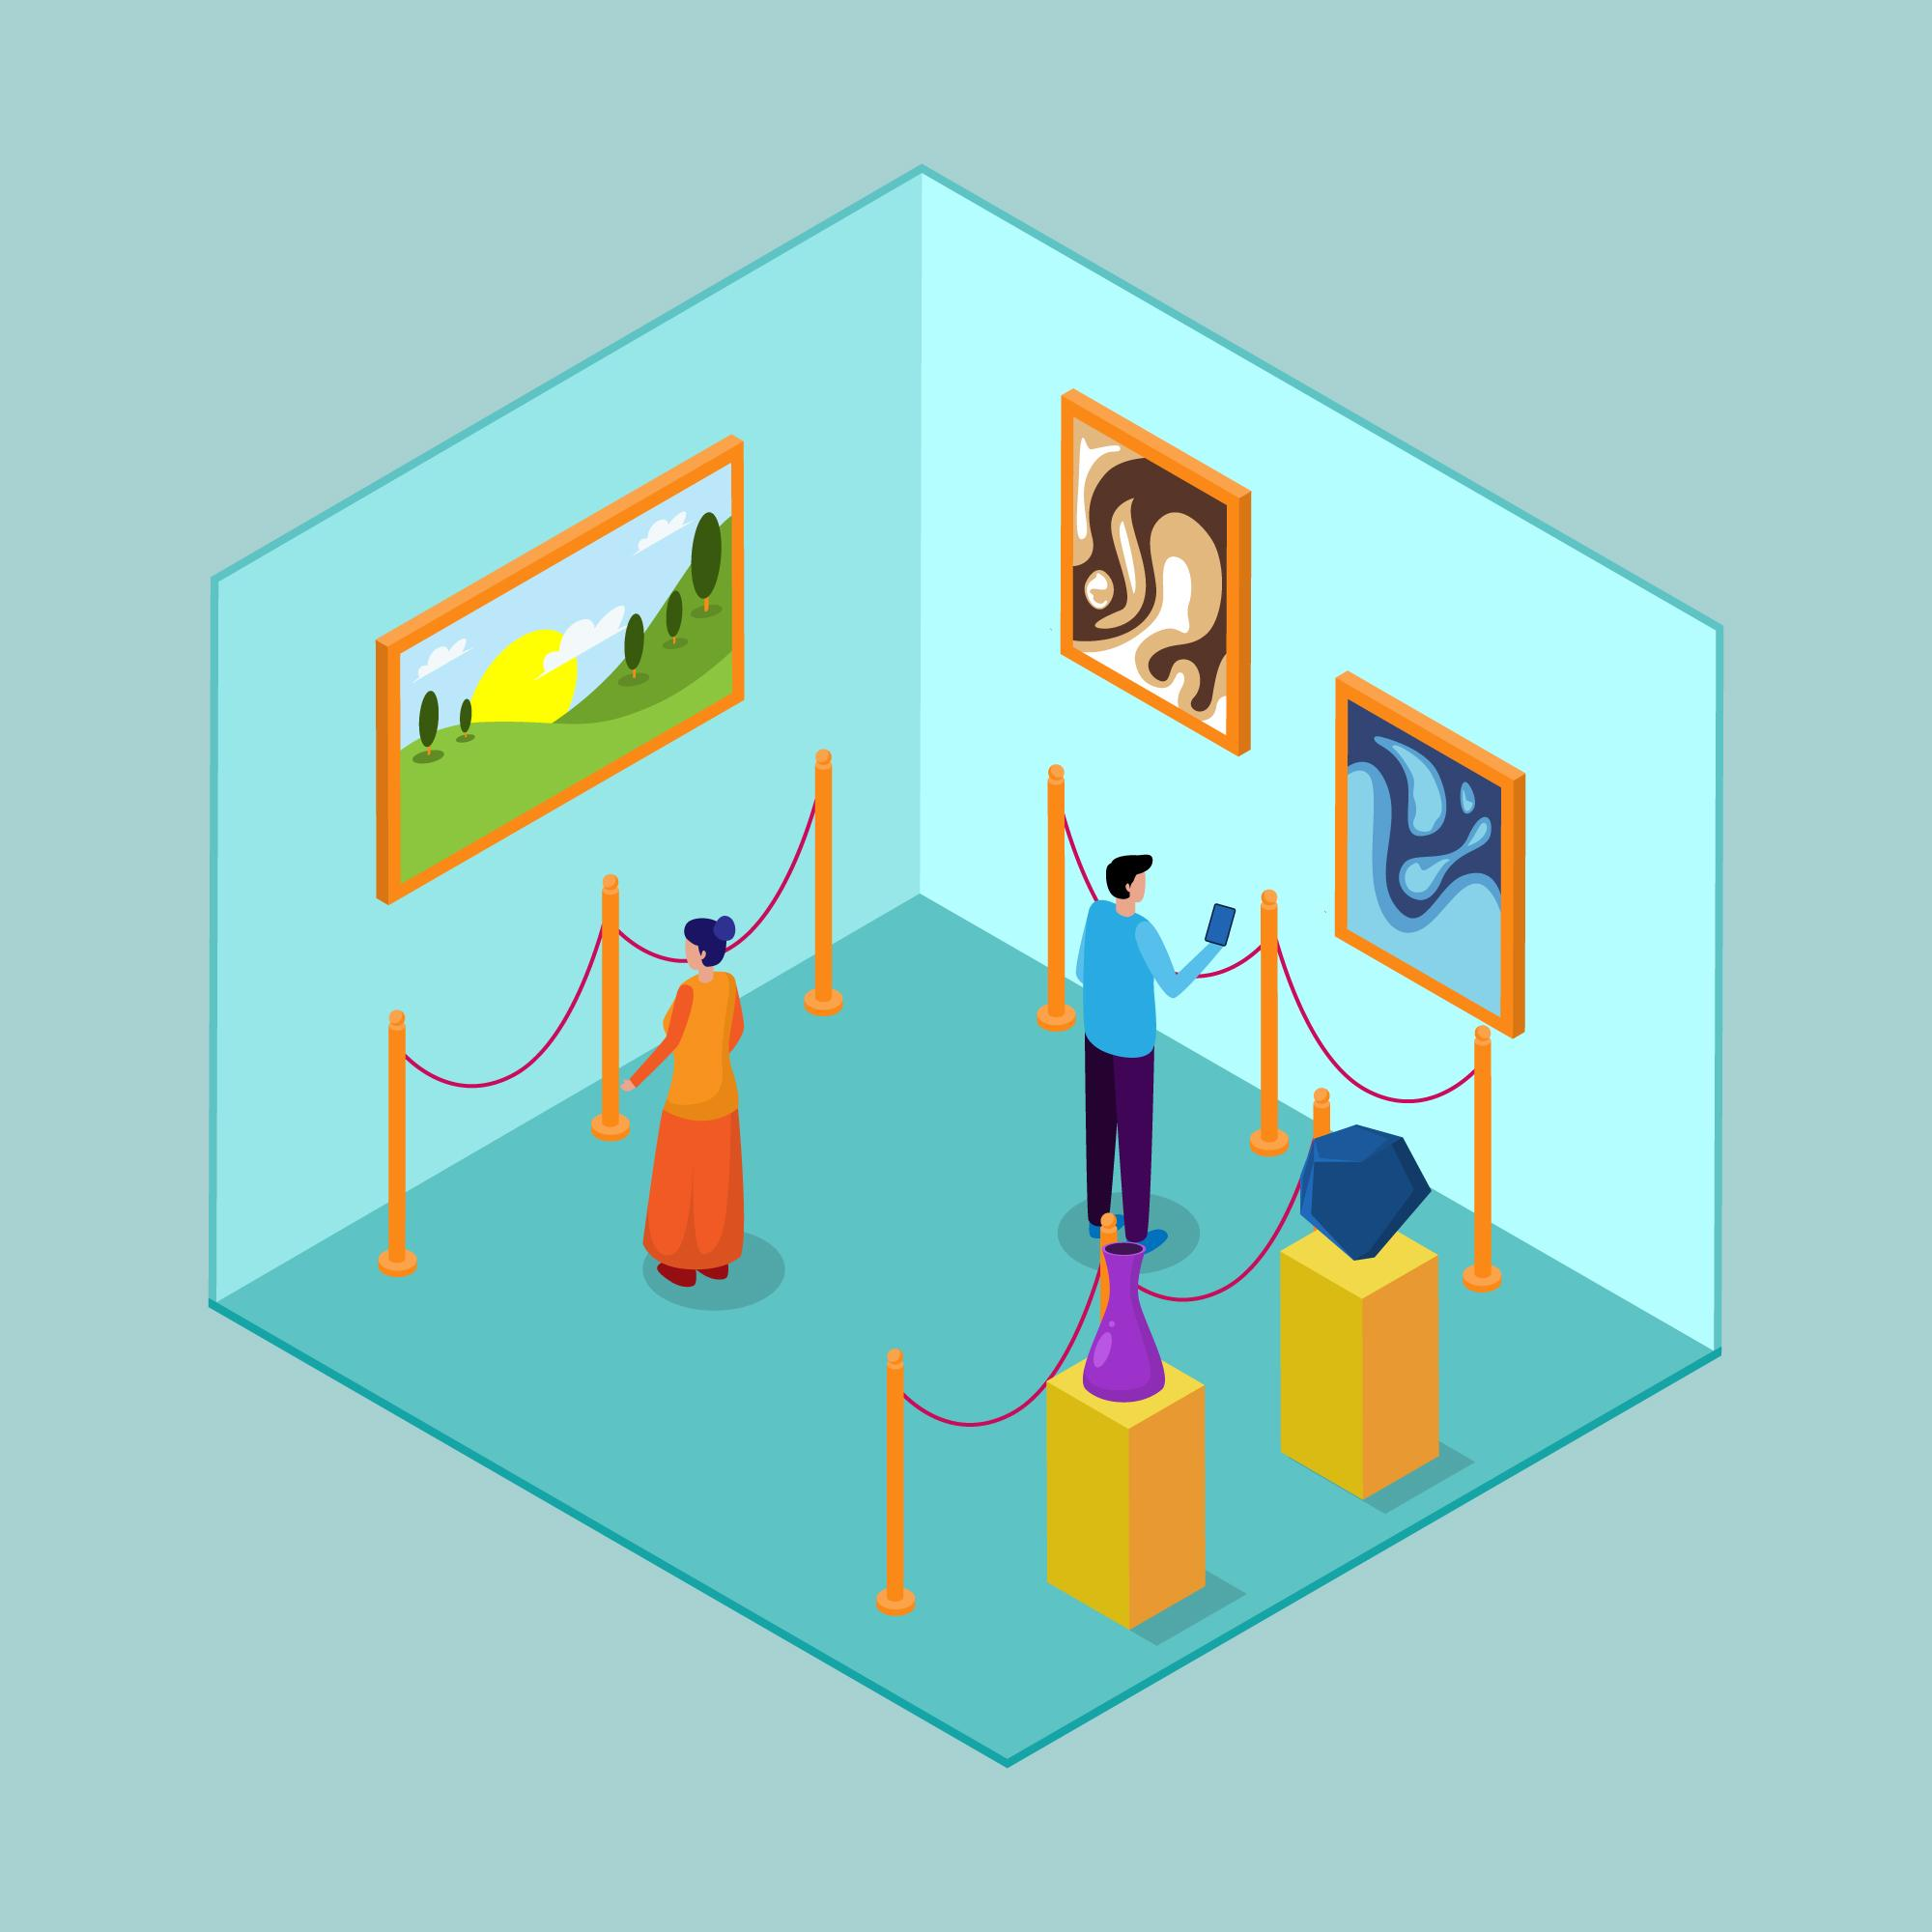
\includegraphics[width=.5\textwidth]{media/image14c.jpeg}
\end{center}

\reduline{Cada seção pode ter no mínimo 6 obras de arte. Logo: 108 x 6 = 648 obras de arte no mínimo na exposição toda. Cada seção pode ter no máximo 9 obras de arte. Logo: 108 x 9 = 972 obras de arte no máximo na exposição toda.\hfill}

\item Um estádio de futebol pequeno tem, na arquibancada superior, 66 fileiras de 302 assentos. Calcule a lotação máxima da arquibancada superior desse estádio.
\reduline{São 66 fileiras x 302 assentos = 19.932 assentos no total.\hfill}
\end{escolha}

\num{6} O pai de Marcela trabalha em uma transportadora e, em determinado
dia, seu caminhão foi carregado com 64 engradados de refrigerantes.
Em cada engradado, há 12 garrafas de refrigerante. Cada garrafa de refrigente
contém 2 litos. Quantos litros de refrigerante o pai de Marcela tinha em seu caminhão?

\reduline{64 x 12 x 2 = 1.536 litros de refrigerante.\hfill}

\num{7} Arnaldo faz dez anos no próximo sábado. Para comemorar seu 
aniversário, os pais dele prepararam uma festa surpresa.
Convidaram todos os amigos de Arnaldo. Para calcular a quantidade 
de doces e salgados que teriam de encomendar, consideraram 6 doces e 
5 salgados por convidado. Sabendo que os pais de Arnaldo,
convidaram 117 pessoas, responda as perguntas a seguir.

\begin{center}

\includegraphics[width=.5\textwidth]{media/image14d.jpeg}
\end{center}

\begin{escolha}
\item Quantas unidades de doces foram encomendadas?
\reduline{Foram encomendadas 6 x 117 = 702 unidades de doces.\hfill}

\item Quantas unidades de salgados foram encomendadas
\reduline{Foram encomendadas 5 x 117 = 585.\hfill}

\item Quantas unidades de doces e salgados foram encomendadas no total?
\reduline{Foram encomendadas (5 + 6) x 117 = 1.287 unidades de doces e salgados.\hfill}
\end{escolha}

\begin{comment}
\begin{minipage}{.5\textwidth}
João possui uma distribuidora de ovos e acabou de receber 14 caixas com 310
ovos cada uma. Para que João venda essa mercadoria, ele faz embalagens
de 12 ovos. Quantas embalagens João conseguirá fazer para
colocar à venda os ovos que acabou de receber? Haverá alguma sobra?
\end{minipage}\hspace{.5cm}
\begin{minipage}{.5\textwidth}
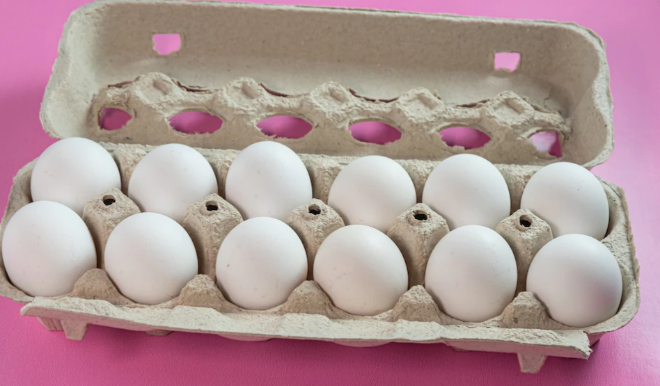
\includegraphics[width=\textwidth]{media/image15.png}
\end{minipage}

\reduline{(14 x 310) : 12 = 361 embalagens com 12 ovos cada uma e uma sobra de 8
ovos.\hfill}

%\coment{Professor, sempre escreva a expressão formada pela interpretação do
%enunciado, pois assim os alunos vão aprendendo a transformar textos em linguagem
%matemática.}
\end{comment}

\num{8} O livro que Gabriel está lendo possui 12 capítulos com 22 páginas cada
um. Se ele ler 10 páginas por dia, em quantos dias ele terminará de ler
o livro?

\reduline{Realizando o cálculo, (12 x 22) : 10 = 26 dias lendo 10 páginas por dia e 1 dia lendo 4 páginas; portanto terminará o livro em 27 dias.\hfill}

\num{9} O pai de Pedro propôs a ele um grande desafio:
o pai fornece uma conta com um número escondido e o filho 
descobre qual número está escondido. Ajude Pedro com esse desafio e
encontre o número que está escondido pelo ponto de interrogação.

\begin{figure}[htpb!]
\centering
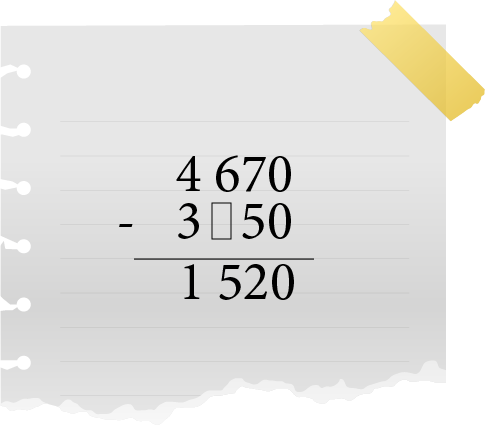
\includegraphics[width=.7\textwidth]{media/image16.png}
\end{figure}

\reduline{O algarismo escondido é o 1.\hfill}

\num{10} Na fazenda do avô de Vinícius, há 104 galinhas, 62 porcos, 6 cavalos e 72
bois. Se na fazenda de seu vizinho o número de animais é o triplo do que
há na fazenda do avô, quantos animais existem na fazenda do
vizinho?

\reduline{Número de animais na fazenda do avô é 104 + 62 + 6 + 72 = 244 animais; e na fazenda do vizinho 244 x 3 = 732 animais.\hfill}

\section*{Treino}


\num{1} O pai de Júlia possui dois veículos de transporte. 
Um é uma caminhote com capacidade de fazer até 15 viagens por dia; 
e outro, maior, consegue realizar 10 viagens. Quantas viagens o pai de 
Julia consegue realizar em um mês, supondo que o mês tenha 
30 dias?

\begin{multicols}{2}
\begin{escolha}
\item 560.

\item 750.

\item 760.

\item 820.
\end{escolha}
\end{multicols}

\num{2} Camila fez um colar com pedras brasileiras. 
Para cada conta de ametista (lilás), ela usou 4 águas-marinhas (azul).
Ela usou 40 pedras ao todo. Quantas pedras liláses e quantas pedras azuis Camila utilizou?

\begin{multicols}{2}
\begin{escolha}
\item 6 liláses, 34 azuis.

\item 8 liláses, 30 azuis. 

\item 6 liláses, 34 azuis.

\item 8 liláses, 32 azuis.
\end{escolha}
\end{multicols}

\num{3} Numa pequena cidade do interior de São Paulo, há um parque de diversões muito conhecido que atrai um grande público. Logo pela manhã, antes mesmo de o parque abrir, já está organizada uma fila de pessoas na entrada. Mas o parque só pode atender a no máximo 2.000 por vez. A partir daí, só entra o número de pessoas correspondenta às que saírem. Nesta quinta, entraram 723 pessoas, mas ainda havia 1.557 pessoas na fila. Quantas pessoas terão de esperar até que comecem sair os primeiros visitantes?

\begin{figure}[htpb!]
\centering
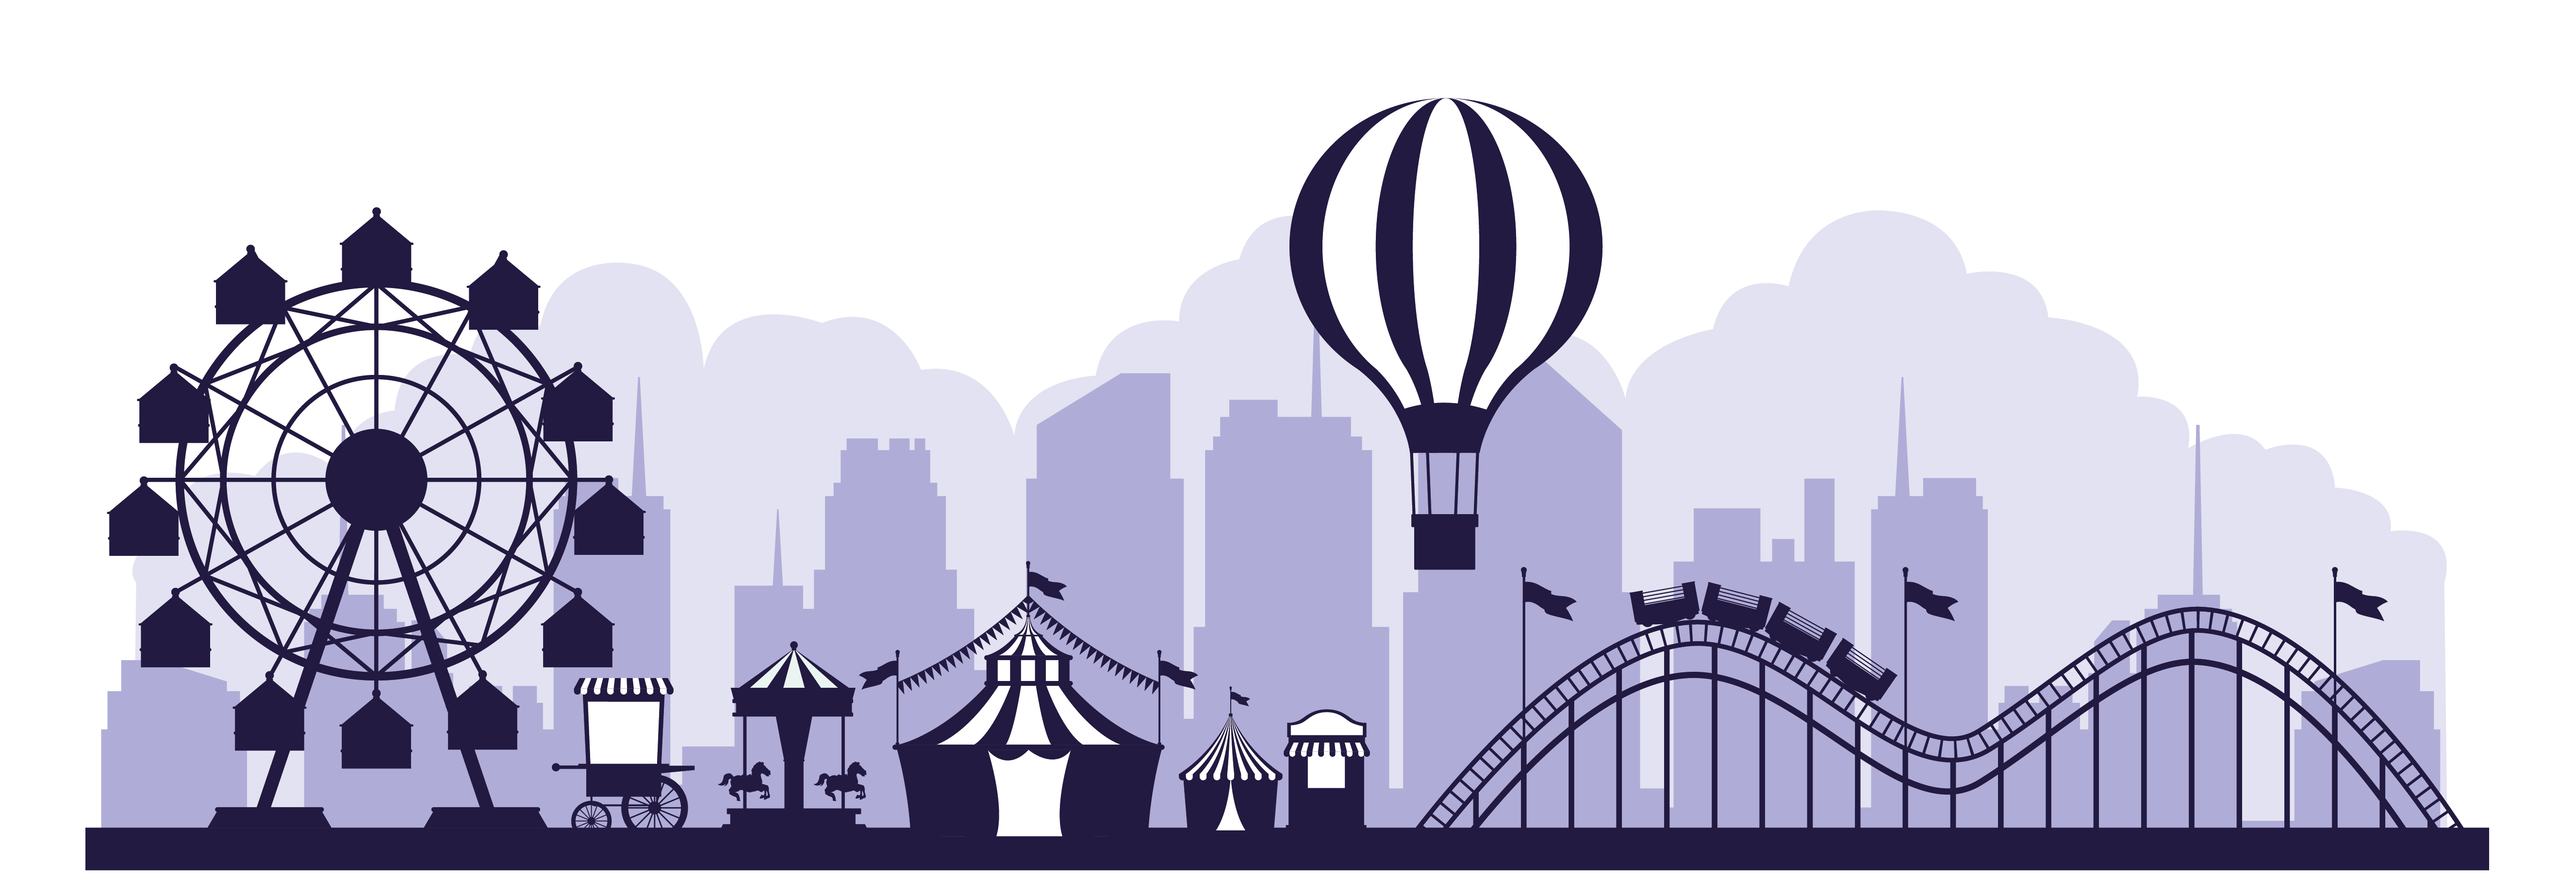
\includegraphics[width=.7\textwidth]{media/image16a.jpeg}
\end{figure}

\begin{multicols}{2}
\begin{escolha}
\item 279.

\item 280.

\item 260.

\item 150.
\end{escolha}
\end{multicols}



\begin{comment}
\num{1} Verificando algumas atividades realizadas na escola no ano anterior,
Gustavo se deparou com uma conta em que 417 era o minuendo, mas o subtraendo
estava coberto por um retângulo. A diferença estava visível: 105.
Gustavo ficou curioso e resolveu refazer a atividade para descobrir o
número que faltava e, após alguns minutos, conseguiu descobrir. O número
que Gustavo encontrou é o

\begin{multicols}{2}
\begin{escolha}
\item
  128.
\item
  312.
\item
  158.
\item
  256.
\end{escolha}
\end{multicols}

\num{2} Isaac estava conferindo o estoque de mercadorias de sua loja e percebeu
que inicialmente ele tinha 200 peças. Depois vendeu 2 caixas com peças
para Carlos. Em cada uma das caixas havia um pacote com 5 unidades de peças e dois
pacotes com 7 peças. Para saber a quantidade de peças que restavam no estoque, Isaac fez a
seguinte anotação:

\begin{myquote}
200 -- 2 x (1 x 5 + 2 x 7)
\end{myquote}

O resultado dessa expressão era exatamente igual à quantidade de peças
que restavam em seu estoque após a venda para Carlos. Qual é a
quantidade de peças que Isaac possui agora em seu estoque?

\begin{multicols}{2}
\begin{escolha}
\item
  72.
\item
  94.
\item
  126.
\item
  162.
\end{escolha}
\end{multicols}

\num{3} Um grande circo chegou à cidade em que Rafael mora, e logo uma fila
enorme se formou com pessoas querendo assistir ao espetáculo. Os
ingressos começaram a ser vendidos e as pessoas começaram a entrar no
recinto do circo. Em certo instante sabia-se que 540 pessoas já tinham
entrado e que a capacidade máxima por espetáculo nesse circo era de 1.200 pessoas. Ainda estão na fila 932 pessoas. Quantas pessoas não
conseguirão entrar para assistir a essa sessão do circo?

\begin{multicols}{2}
\begin{escolha}
\item
  268.
\item
  272.
\item
  294.
\item
  440.
\end{escolha}
\end{multicols}

\end{comment}
\chapter{Sequências}
\markboth{Módulo 3}{}

\section*{Habilidades do SAEB}

\begin{itemize}
\item Inferir ou descrever atributos ou propriedades comuns que os elementos
que constituem uma sequência recursiva de números naturais apresentam.

\item Inferir o padrão ou a regularidade de uma sequência de números
naturais ordenados, objetos ou figuras.

\item Inferir os elementos ausentes em uma sequência de números naturais
ordenados, objetos ou figuras.
\end{itemize}

\subsection{Habilidade da BNCC}

\begin{itemize}
\item EF04MA11.
\end{itemize}

\conteudo{
Uma sequência ou sucessão é um conjunto ordenado no qual
há uma lógica de composição. 
\bigskip

Veja exemplos a seguir.

\begin{itemize}
\item
  A escalação de um time de vôlei, com seis jogadores em quadra, pode ser apresentado em ordem alfabética: Antonio; Barão; Cláudio, Danilo, Eduardo e Fernando.
\item
  Uma sequência pode ser formadada pelo números naturais pares: 0, 2, 4, 6, 8, 10, 12...
\end{itemize}
\bigskip

Uma sequência pode apresentar termos

\begin{itemize}
\item
  \textbf{finitos}, isto é, uma quantidade de termos definidos.
\item
  \textbf{infinitas}, isto é, infinitos termos, como
  a sequência dos números naturais: 1, 2, 3, 4, 5, 6, 7, 8, 9...
\end{itemize}
\bigskip
\pagebreak

Uma sequência também pode apresentar ordem:

\begin{itemize}
\item
  \textbf{crescente}, isto é, o termo sucessor deve ser maior que seu
  antecessor. Por exemplo: 5, 10, 15, 20, 25.
\item
  \textbf{decrescente}, isto é, o termo sucessor deve ser menor que
  seu antecessor. Por exemplo: 9, 7, 5, 3.
\end{itemize}
}

\section*{Atividades}

\num{1} Encontre o número pedido em cada item a seguir.

\begin{escolha}
\item
  O sucessor de 999: \reduline{1.000.\hfill}

\item
  O antecessor de 4.398: \reduline{4.397.\hfill}

\item
  O sucessor e o antecessor do número 99.259: \reduline{99.258 e 99.260.\hfill}
\end{escolha}


\num{2} Relembre os conceitos de números naturais pares e ímpares e, em seguida,
responda ao que se pergunta.

\begin{escolha}
\item
  Escreva os 10 primeiros números naturais pares em sequência crescente.
  Essa sequência é finita ou infinita? Como ela é formada?
\reduline{(0; 2; 4; 6; 8; 10; 12; 14; 16; 18). Essa é uma sequência finita e sempre
somamos 2 ao termo anterior para encontrar o próximo.\hfill}

\item
  Escreva os 12 primeiros números naturais ímpares em sequência
  crescente. Essa sequência é finita ou infinita? Como ela é formada?
\reduline{(1; 3; 5; 7; 9; 11; 13; 15; 17; 19; 21; 23). Essa é uma sequência finita
e sempre somamos 2 ao termo anterior para encontrar o próximo.\hfill}
\end{escolha}

%\coment{Explore com os alunos o conceito de que, na sequência dos números naturais, após um número par sempre aparece um numero ímpar, ou seja, eles se intercalam.}

\pagebreak
\num{3} Monte cada uma das sequências propostas a seguir, com seis números cada uma.

\begin{escolha}
\item
  Sequência de números que começa no 222 e aumenta de 9 em 9 unidades.
\reduline{(222; 231; 240; 249; 258; 267).\hfill}

\item
  Sequência de números que começa no 30 e aumenta de 50 em 50 unidades.
\reduline{30; 80; 130; 180; 230; 280.\hfill}

\item
  Sequência de números que começa no 220 e diminui de 5 em 5 unidades.
\reduline{220; 215; 210; 205; 200; 195.\hfill}
\end{escolha}


\num{4} Observe as sequências dadas e determine o oitavo termo.

\begin{escolha}
  \item (7; 14; 21...) \reduline{8 x 7 = 56.\hfill}

  \item (9; 18; 27...) \reduline{8 x 9 = 72.\hfill}

  \item (6; 12; 18...) \reduline{8 x 6 = 48.\hfill}
  \end{escolha}


\num{5} Organize os números a seguir em ordem decrescente.

\begin{figure}[htpb!]
\centering
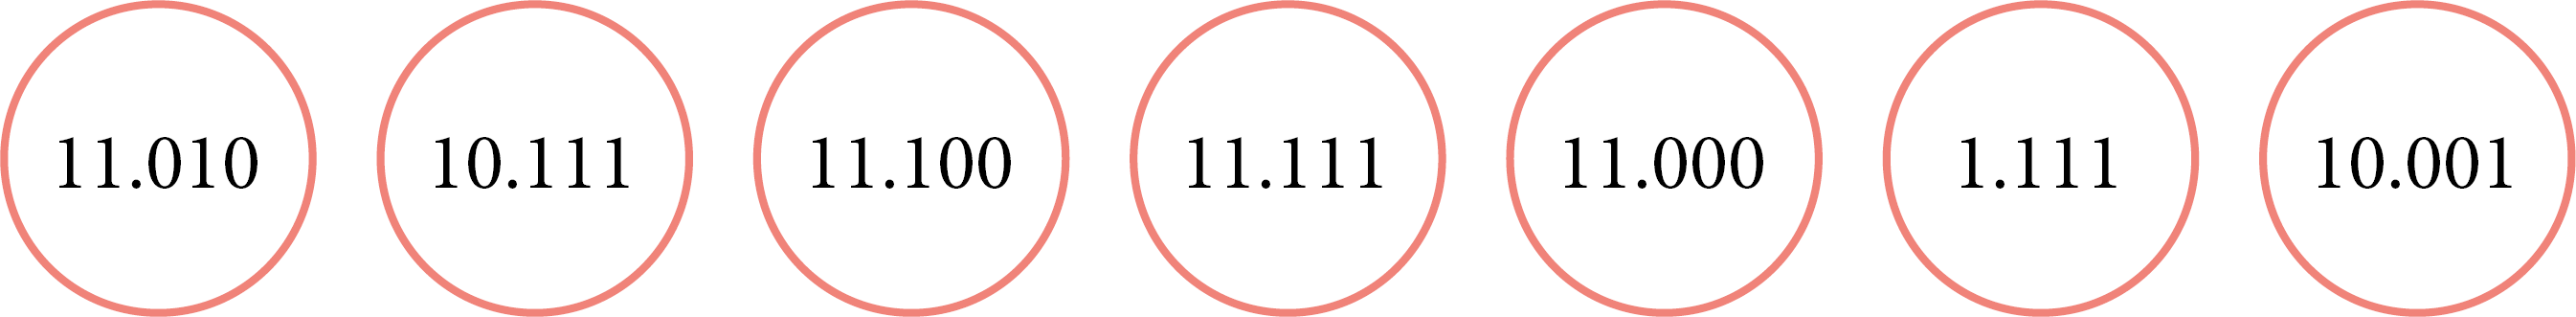
\includegraphics[width=\textwidth]{media/image18.png}
\end{figure}

\reduline{Ordem decrescente (do maior para o menor):
11.111; 11.100; 11.010; 11.000; 10.111; 10.001; 1.111.\hfill}


\num{6} Observe as sequências a seguir e as complete com os números que estão
faltando.

\begin{escolha}
\item 5.862 \quad 6.862 \quad 7.862 \quad \reduline{8.862\hspace{1cm}}\quad \reduline{9.862\hspace{1cm}} \quad 10 862

\item 198 \quad 190 \reduline{182\hspace{1cm}}\quad 174 \reduline{166\hspace{1cm}}\quad \reduline{158\hspace{1cm}}
\end{escolha}

\pagebreak
\num{7} Observe atentamente a sequência numérica que Robson construiu e depois
faça o que se pede.

\begin{figure}[htpb!]
\centering
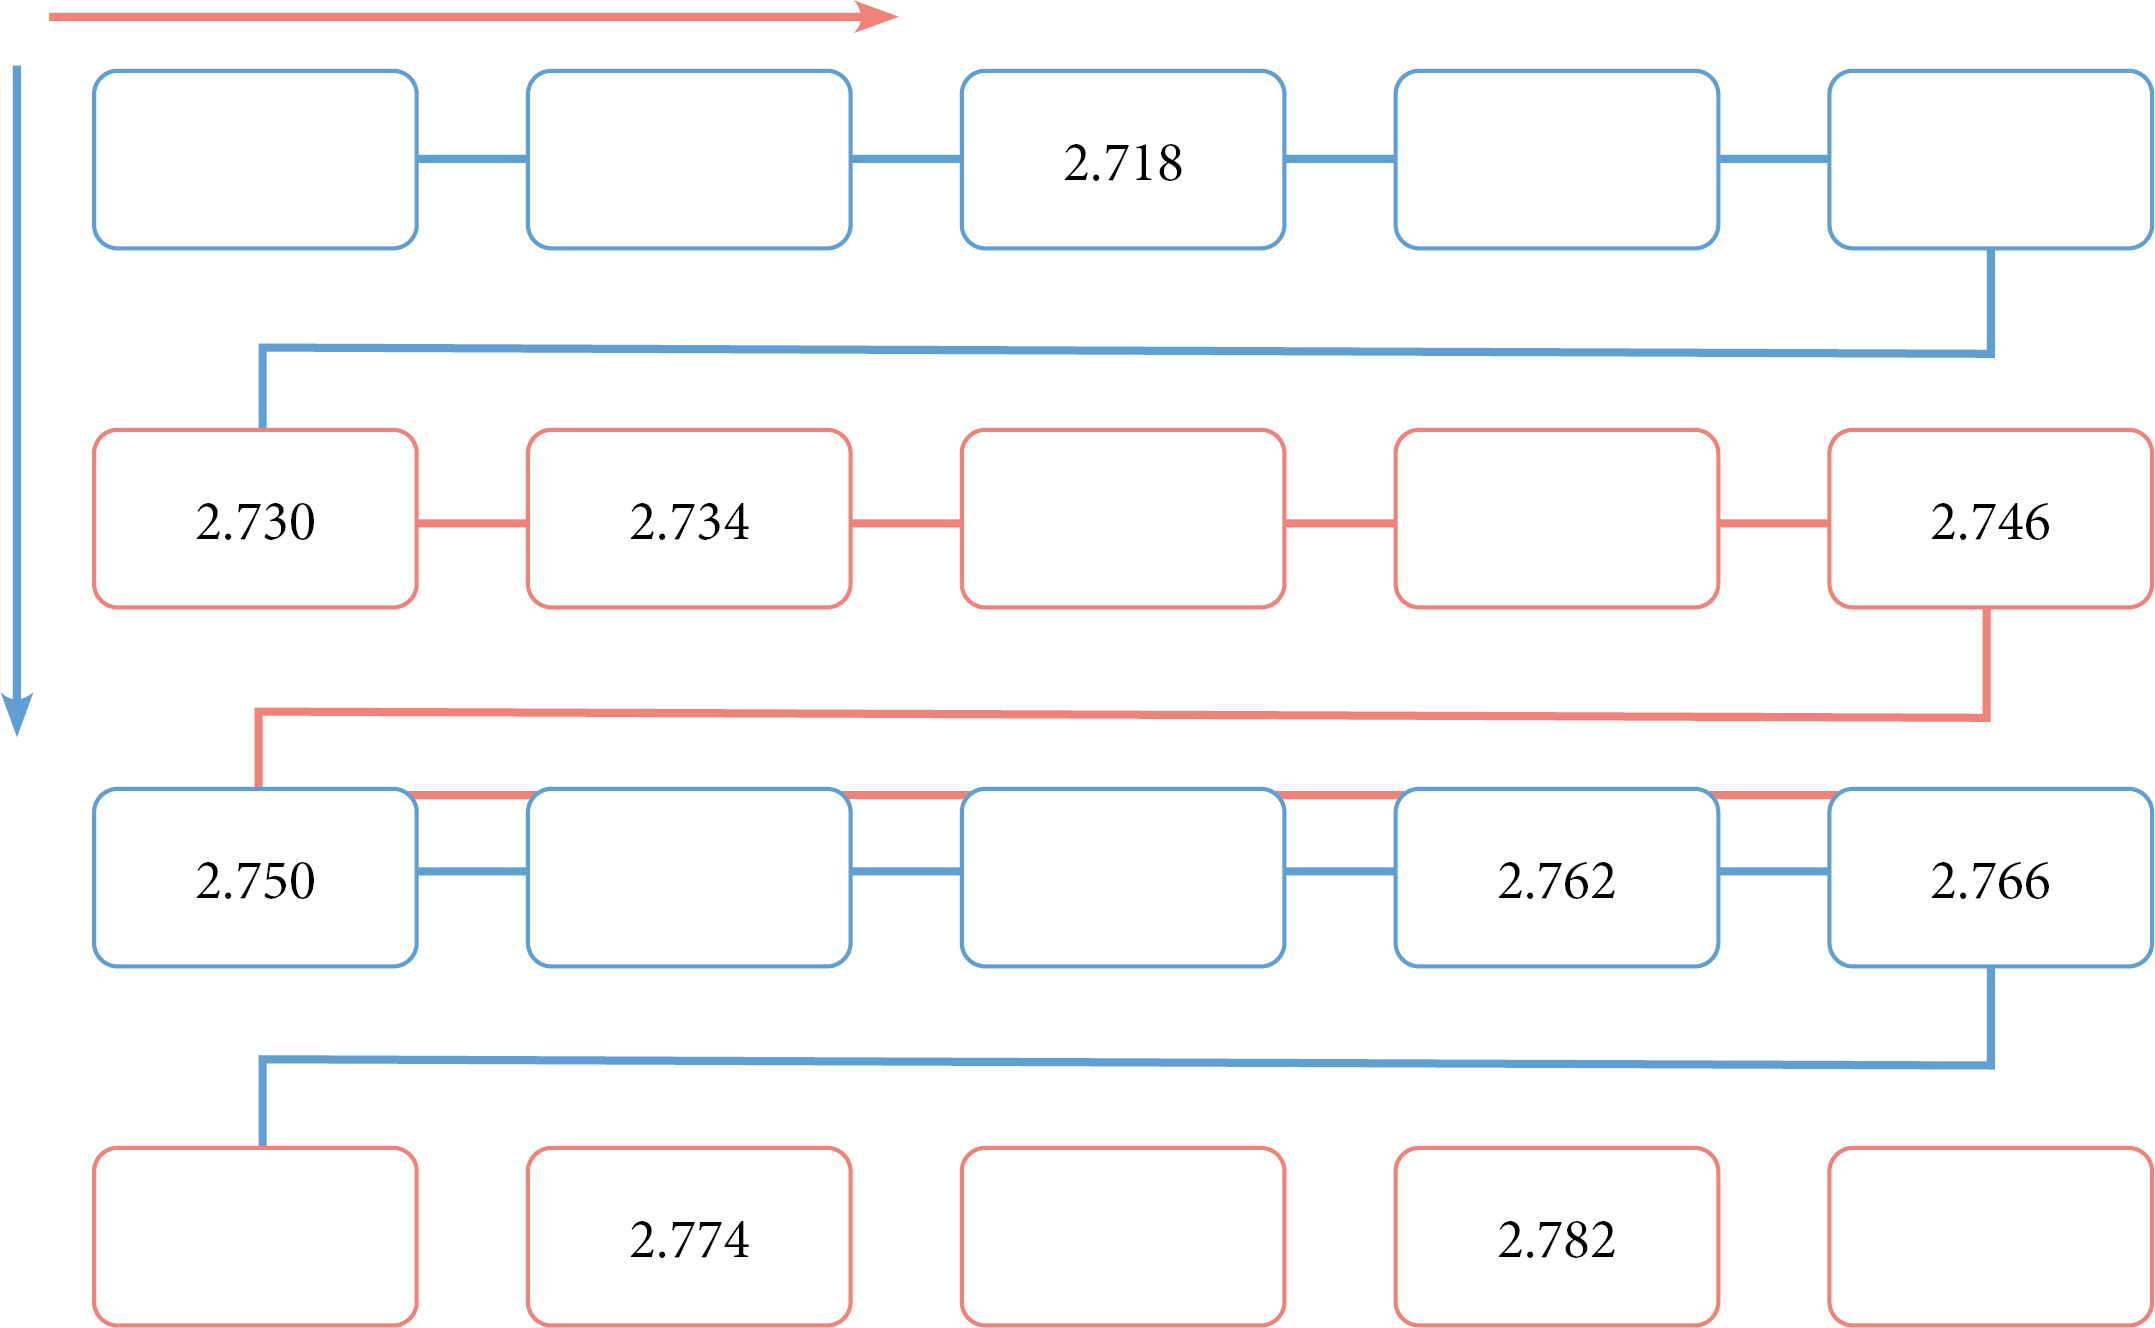
\includegraphics[width=\textwidth]{media/image17.png}
\end{figure}

\begin{escolha}
\item
  Qual é lógica Robson utilizou para construir essa sequência?
\reduline{Em cada coluna, ele foi aumentando os números na ordem de 10 unidades, enquanto,
em cada linha, o aumento foi de 4 unidades. Outra forma de pensar é que, seguindo as setas colocadas por ele, o aumento foi de 4 unidades de um número para o próximo.
Professor, explore as duas situações com os alunos.\hfill}
\linhas{1}

\item
  Complete a sequência com os números que estão faltando.

\reduline{\textbf{Linha 1}: 2.710; 2.714; 2.718; 2.722; 2.726. \textbf{Linha 2}: 2.730; 2.734; 2.738; 2.742; 2.746. \textbf{Linha 3}: 2.750; 2.754; 2.758; 2.762; 2.766. \textbf{Linha 4}: 2.770; 2.774; 2.778. 2.782; 2.786.\hfill}
\linhas{2}
\end{escolha}

\num{8} Victor leu uma notícia sobre os Jogos Olímpicos. 
Pelo texto, ele aprendeu que o evento poliesportivo ocorre a cada quatro anos, 
sediados sempre por um país diferente do anterior. 
Ele também ficou sabendo de que a primeira edição do século XXI ocorreu em 2004. 
Quantas são as sedes do evento entre 2004 e 2024? 

\begin{figure}[htpb!]
\centering

\includegraphics[width=.4\textwidth]{media/image17a.jpeg}
\end{figure}

\reduline{Os Jogos Olímpicos de 2004 a 2024 foram sediados em Atenas (2004), 
Pequim (2008), Londres (2012), Rio de Janeiro (2016), Tóquio (2020) 
e Paris (2024). Portanto, são seis sedes.}  

\begin{comment}
Entre os cadernos de seu irmão, Ana Clara encontrou um papel 
em que estava escrito assim: (231; 288; 245; 402; ...). Ela ficou muito curiosa, 
pois entendeu que essa era uma sequência numérica, 
e queria encontrar o próximo número. Ajude Ana Clara a descobrir qual 
é o próximo número da sequência e o escreva no espaço a seguir.

\reduline{A sequência foi montada sempre somando-se 57 ao número anterior para
encontrar o próximo. Portanto, o próximo número da sequência será: 402 +
57 = 459.\hfill}
\linhas{1}
\end{comment}


\num{9} Estudando com a filha, Luísa, para a prova de Matemática da semana seguinte,
Laura propõe à menina o exercício a seguir.

Escreva uma sequência de 6 números que aumenta de 12 em 12 unidades,
começando pelo número nove mil e novecentos e noventa e nove.

Ajude Luísa a resolver esse exercício, escrevendo os seis números
pedidos.

\reduline{A sequência é: 9.999; 10.011; 10.023; 10.035; 10.047; 10.059.\hfill}

\num{10} O Pai de André montou a sequência de figuras a seguir.

\begin{figure}[htpb!]
\centering

\includegraphics[width=.7\textwidth]{media/image19.png}
\end{figure}

Em seguida, disse ao filho que o levaria ao cinema caso ele acertasse
qual seria o 20º termo dessa sequência. André, muito empolgado, começou a
pensar e logo deu a resposta a seu pai. O pai analisou a resposta e
disse que estava correta. Qual é a resposta que André deu a seu pai?

\reduline{A sequência segue um padrão no qual dois retângulos consecutivos 
são seguidos por um triângulo. Isso significa que os termos pares são 
retângulos e os termos ímpares são triângulos. O 20º termo é par, portanto, será um retângulo.\hfill}

%\reduline{É possível que o aluno continue a sequência com desenhos até
%chegar à resposta. Não há problema nisso, e é muito válido, pois assim
%entenderão a lógica envolvida.\hfill}


\pagebreak
\section*{Treino}

\begin{comment}
\num{1} Observe a sequência a seguir.

\begin{quote}
\begin{itemize}
  \item Figura 1: duas bolinhas.
  \item Figura 2: seis bolinhas.
  \item Figura 3: doze bolinhas.
  \item Figura 4: vinte bolinhas.
\end{itemize}
\end{quote}

 A figura 6 terá

\begin{escolha}
\item
  25 bolinhas.
\item
  30 bolinhas.
\item
  35 bolinhas.
\item
  42 bolinhas.
\end{escolha}
\end{comment}

\num{1} Marcos escreveu números os números a seguir no seu caderno: 74, 101.111, 2, 888, 217, 13. Ajude-o a colocá-los em ordem decrescente.  

\begin{escolha}
\item 111.101, 888, 217, 74, 13, 2.

\item 101.101, 888, 271, 74, 13, 2.

\item 101.111, 888, 217, 47, 13, 2.

\item 101.111, 888, 217, 74, 13, 2.
\end{escolha}

\num{2} Ana Amélia encontrou a seguinte sequência numérica e ficou curiosa, pois
faltava um número para ser escrito.

\begin{mdframed}[linewidth=2pt,linecolor=azul!20,backgroundcolor=azul!20,roundcorner=2pt]
\textbf{45.205 \hfill 45.305 \hfill 45.405 \hfill 45.505 \hfill ? \hfill 45.705 \hfill}
\end{mdframed}

Utilizando seus conhecimentos matemáticos, Ana Amélia chegou à conclusão de que
faltava o número

\begin{escolha}
\item
  45.505.
\item
  45.605.
\item
  45.705.
\item
  45.205.
\end{escolha}

\num{3} Tom utiliza dois cadeados de segredo para prender a bicicleta na escola. 
Para um dos cadeados, ele utiliza a combinação 7081 e, para o outro, o número sucessor. 
A combinação do segundo cadeado é 

\begin{comment}
Dois aplicativos exigem uma senha numérica para serem acessados. Breno
criou a senha 7081 para o primeiro e para o segundo utilizou como senha
o sucessor do sucessor do número escolhido para a primeira senha. A
senha utilizada por Breno para o segundo aplicativo é
\end{comment}

\begin{escolha}
\item
  7079.
\item
  7080.
\item
  7082.
\item
  7083.
\end{escolha}

\chapter{Grandezas e medidas}
\markboth{Módulo 4}{}

\section*{Habilidades do SAEB}

\begin{itemize}
\item Reconhecer a unidade de medida ou o instrumento mais apropriado para
medições de comprimento, área, massa, tempo, capacidade ou temperatura.

\item Estimar/inferir medida de comprimento, capacidade ou massa de objetos,
utilizando unidades de medida convencionais ou não ou medir comprimento,
capacidade ou massa de objetos.

\item Explicar que o resultado de uma medida depende da unidade de medida
utilizada.

\item Resolver problemas que envolvam medidas de grandezas (comprimento,
massa, tempo e capacidade) em que haja conversões entre as unidades mais
usuais.

\item Determinar o horário de início, o horário de término ou a duração de
um acontecimento.
\end{itemize}

\subsection*{Habilidades da BNCC}

\begin{itemize}
\item EF04MA20, EF04MA23.
\end{itemize}

\conteudo{

\textbf{Medindo o mundo ao redor}

Com a adoção do sistema de numeração indo-arábico, 
foi possível estabelecer unidade de medida para tempo, 
espaço, clima, ambiente, coisas, animais ou pessoas.

Uma unidade de medida é uma quantidade estipulada de algo, 
que é uniformizada e divulgada para que todas as pessoas 
saibam e possam usá-la para realizar cálculos, 
obtendo o mesmo resultado.
\bigskip

\noindent{\textbf{Tempo}}

A grandeza de tempo é duração. Ela pode ser indicada em minutos, horas, períodos, dias,
semanas, meses, anos, décadas, séculos. 

\begin{itemize}
\item 60 minutos é a duração de 1 hora. 
\item 24 horas é a duração de 1 dia. 
\item 7 dias é a duração de 1 semana.
\item Os meses podem ter 28, 30 ou 31 dias. E, 
a cada quatro anos o mês de 28 dias, tem 29 dias, 
chamado de ano bisexto.
\item Um ano são 12 meses.
\item 10 anos é a duração de uma década.
\item 100 anos ou 10 décadas é a duração de um século.
\end{itemize}

Em geral, os instrumentos usados para medir o tempo
são: cronômetro, o relógio, a folhinha, entre outros. 
\bigskip

\noindent{\textbf{Espaço}}

Em geral, a medida de espaço é indicada em centímetros, metros, quilômetros.

\begin{itemize}
\item O tamanho de uma borboleta pode variar de 3 a 20 centímetros. 
Abreviação usada para a palavra centímetro é ``cm''. 
\item Um ser humano adulto pode medir 1,75 m ou 175 cm centímetros. 
A abrevição de metro é dada pela letra ``m'' ao lado do número.
\item Em média, um gato doméstico possui 76 cm do focinho à ponta da cauda.
\item Uma régua escolar mede 30 cm. 
\item Muitos livros de literatura apresentam 16 cm de largura por 23 cm de altura.
\item Distância linear entre Oiapoque, no Norte do Brasil, e o Chuí, ao Sul,
é de aproximadamente 4.176 quilômetro, uma das maiores distâncias no território.
\end{itemize}

Os instrumentos mais comuns para medir espaço são
régua, metro, trena, odômetro.  
\bigskip

\noindent{\textbf{Clima}}

A medida mais usada no Brasil para indicar a temperatura ambiente é graus Célsius ou °C. 

\begin{itemize}
\item Temperaturas acima dos 35,5°C foram registradas no inverno de 2023.
\item É pouco comum que se verifique temperaturas abaixo de 30°C durante o verão na região Nordeste.  
\end{itemize}

O termômetro é usado para medir a temperatura. 
Há, porém, termômetros com diferentes finalidades: 
temperatura do ambiente, do corpo ou de um líquido.
\bigskip

\noindent{\textbf{Massa}}

A massa de um corpo é dado em quilos, gramas ou toneladas.

\begin{itemize}
  \item --- O peixe pesou 2 kg, fregueza.
  \item Anderson tem dez anos e pesa 35,4.
  \item Eles não conseguiram mover o objeto de metal que pesou 25 t, mesmo usando um guindaste.
\end{itemize}

A massa de um corpo é medido por uma balança. 
Existe balança para medir a massa de um corpo humano, 
como as encontradas em farmácias; 
há balanças de precisão para corpos muito pequenos;
balanças para medir a massa de objetos, como as de mercado, entre outras.

\noindent{\textbf{Volume ou dimensão}}

Volume ou dimensão de um líquido é indicado em litros ou mililitros. 

\begin{itemize}
  \item Uma embalagem longa vida de leite contém 1 l.
  \item Um garrafão de suco de uva contém 5 l. A abreviação de litro pode ser indicada pela letra ``l'' minúscula ou pela letra ``L'' maiúscula. 
  \item Um copo de tipo americano contém até 190 mililitros ou 190 ml ou mL.
\end{itemize}

  }

\begin{comment}
\begin{itemize}
  \item Medidas de comprimento:
  quilômetro (km), hectômetro (hm), decâmetro (dam), \textbf{metro (m)}, decímetro (dm), centímetro (cm), milímetro (mm).

  \item Medidas de massa:
  quilograma (kg), hectograma (hg), decagrama (dag), \textbf{grama(g)}, decigrama (dg), centigrama (cg), miligrama (mg).

  \item Medidas de capacidade:
  quilolitro (kL), hectolitro (hL), decalitro (daL), \textbf{litro(L)}, decilitro (dL), centilitro (cL), mililitro (mL).

  \item Medidas de tempo:
  1 dia = 24 horas (h) = 1.440 minutos (min) = 86.400 segundos (s).
\end{itemize}
\end{comment}

\section*{Atividades}

\num{1} Relacione as quantidades que estão na coluna da esquerda com a leitura correta
correspondente na leitura da direita.

\begin{figure}[htpb!]
\centering
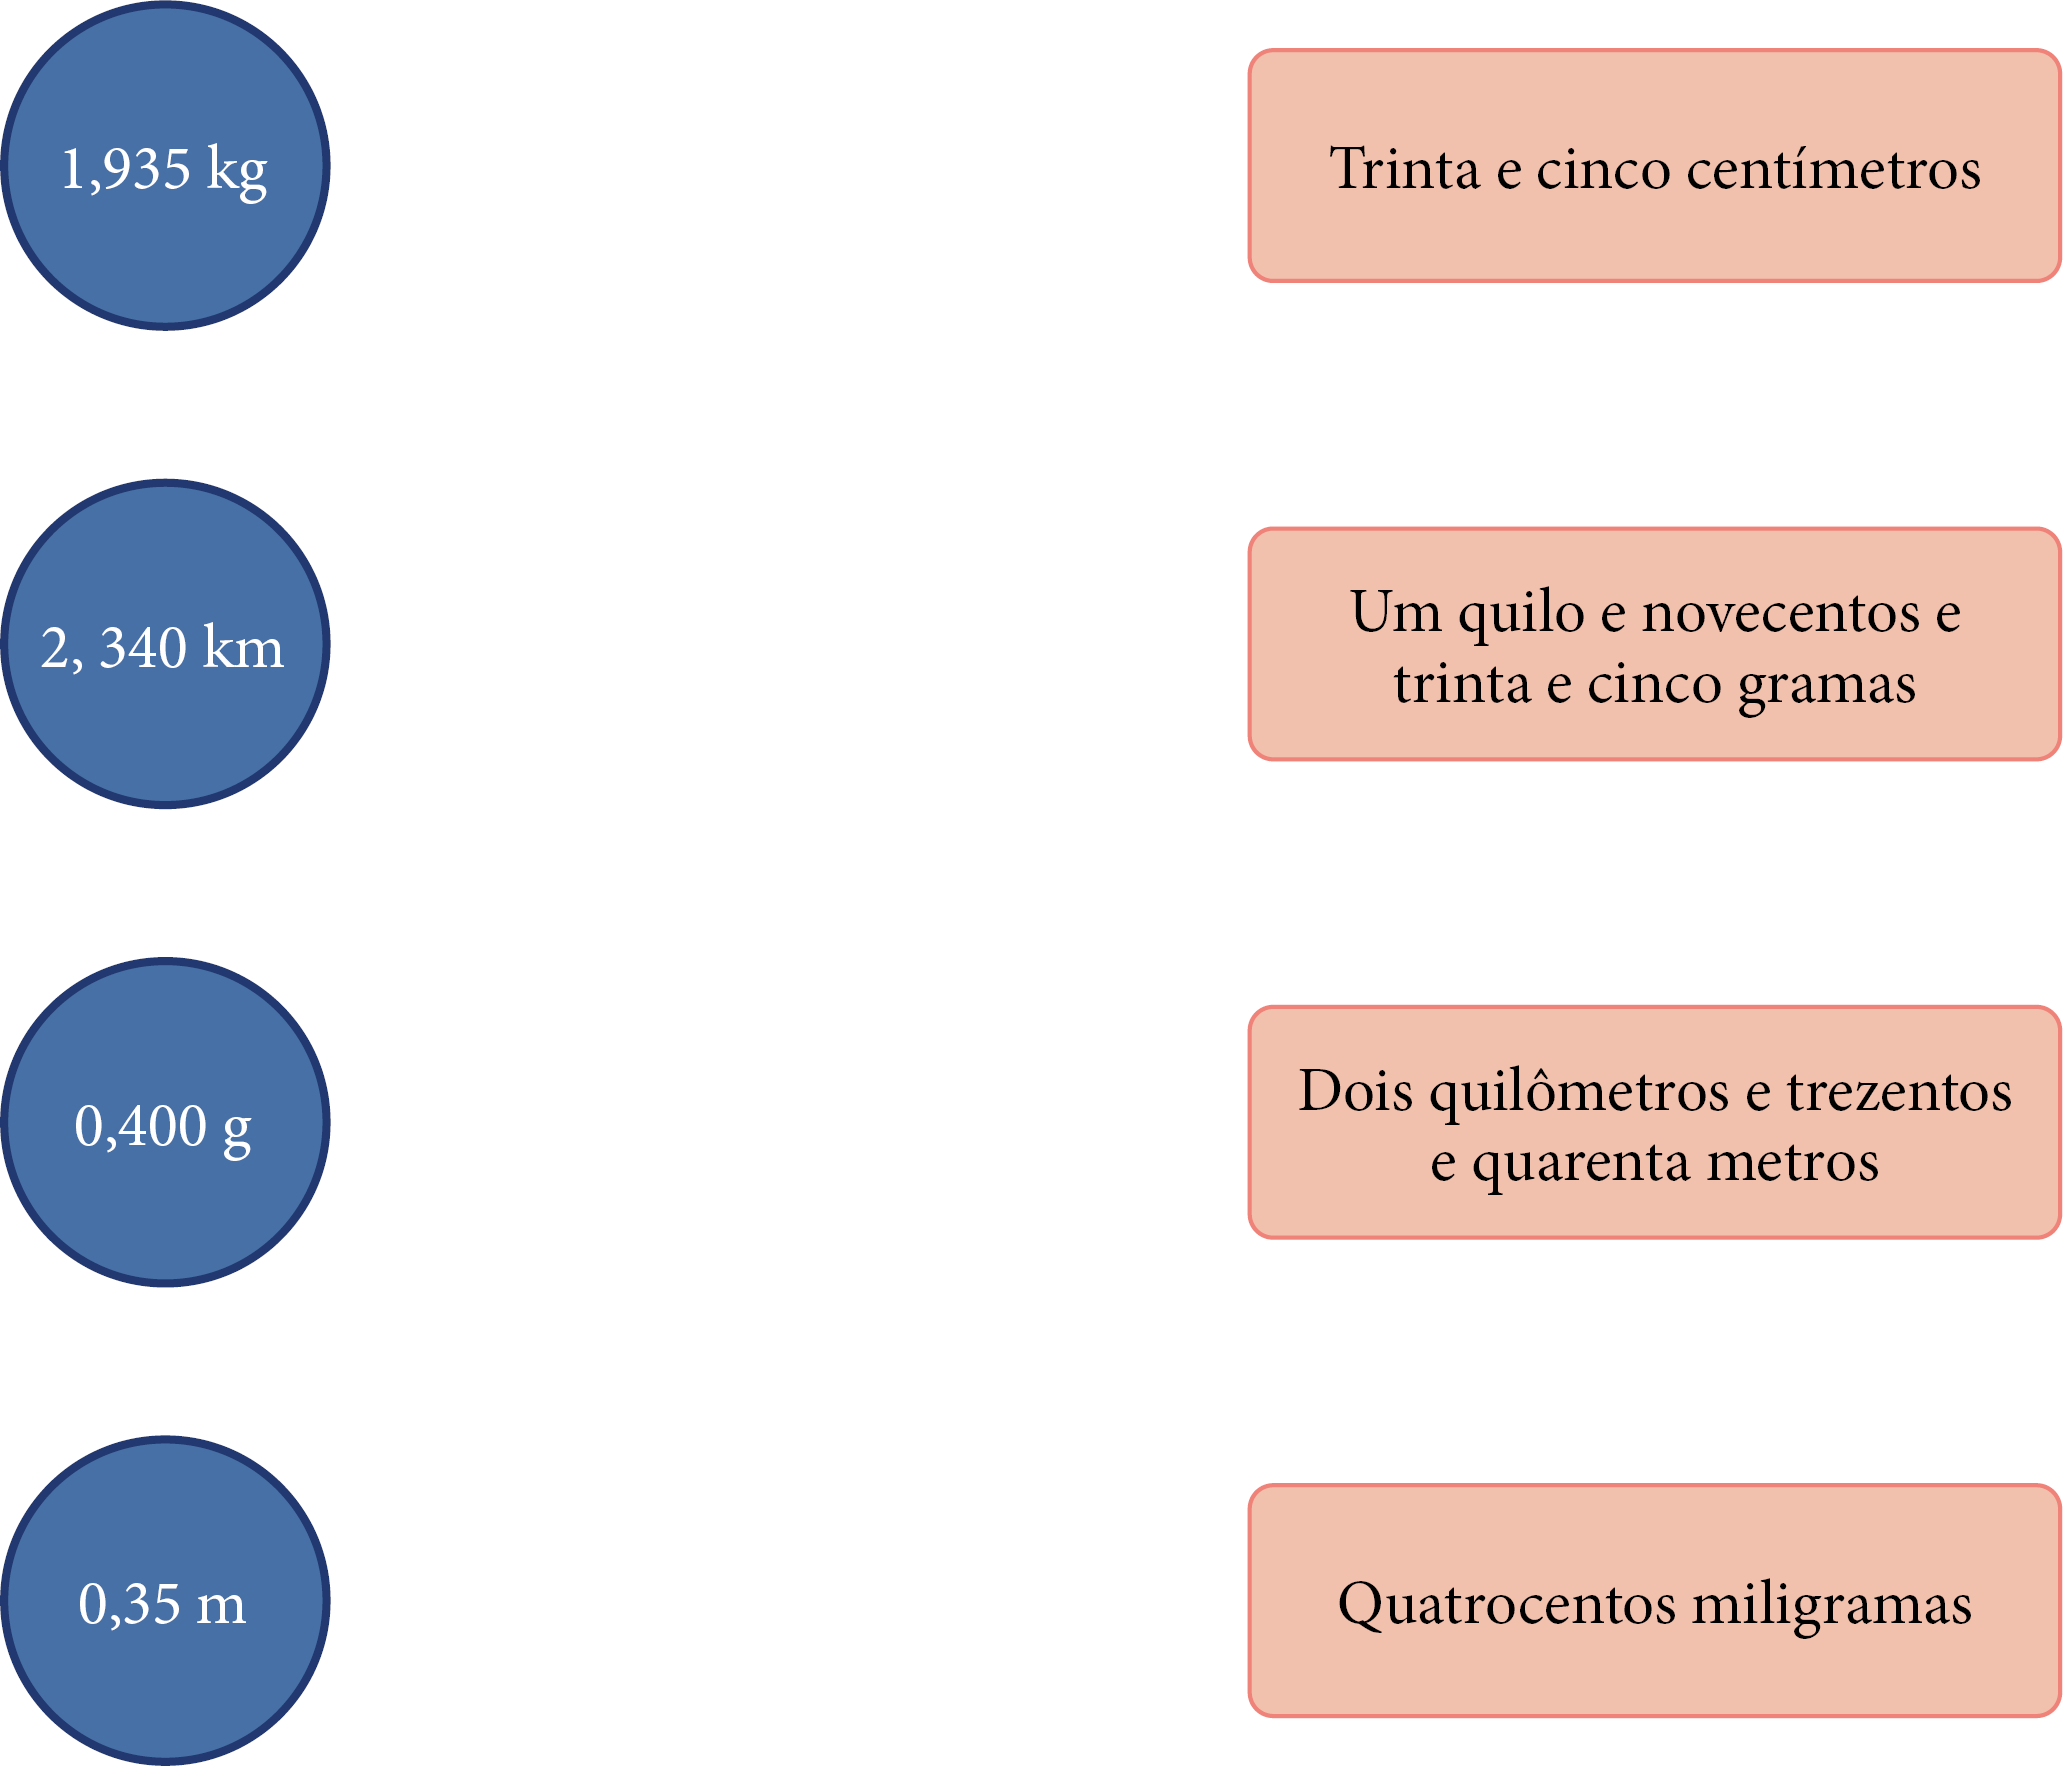
\includegraphics[width=.5\textwidth]{media/image20.png}
\end{figure}

\coment{1,935 kg = um quilo e novecentos e trinta e cinco gramas; 
2,340 km = Dois quilômetros e trezentos e quarenta metros; 
0,400 g = quatrocentos miligramas; 0,35 m = trinta e cinco centímetros.}

\pagebreak
\num{2} Pinte a bolinha que corresponde à capacidade total de líquido que há em cada caso.

\begin{figure}[htpb!]
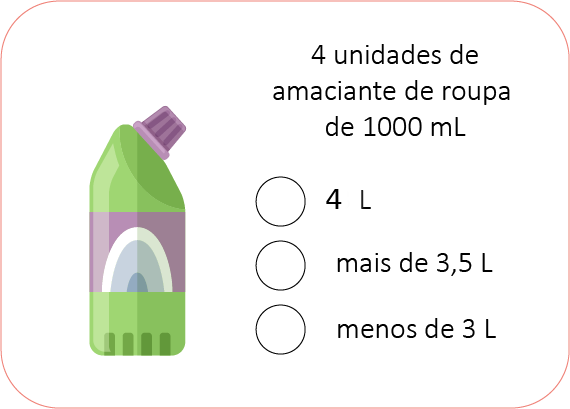
\includegraphics[width=.5\textwidth]{media/image21.png}
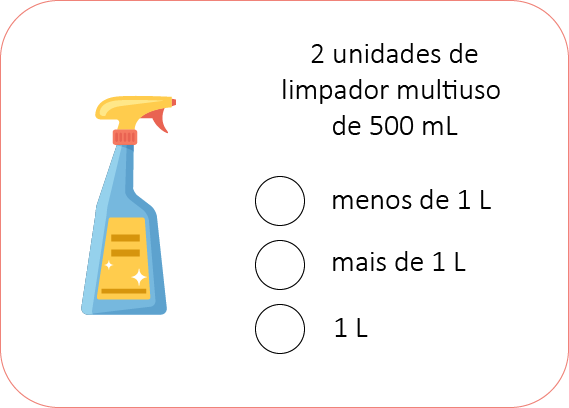
\includegraphics[width=.5\textwidth]{media/image22.png}
\end{figure}

\begin{figure}[htpb!]

\includegraphics[width=.5\textwidth]{media/image23.png}
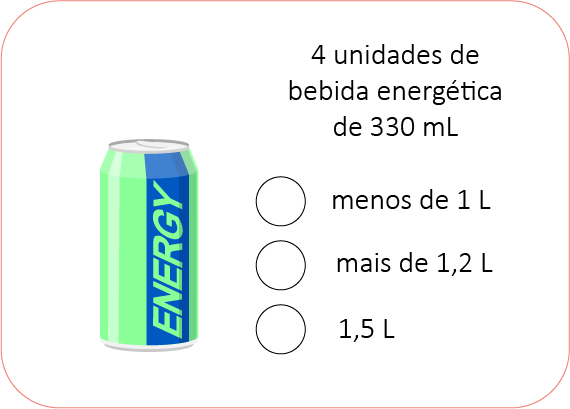
\includegraphics[width=.5\textwidth]{media/image24.png}
\end{figure}

%\coment{Duas unidades de limpador multiuso de 500 mL totalizam 1 litro. Três unidades de loção hidratante de 150 mL totalizam 450 mL (menos que 0,5 L). Quatro unidades de bebida energética de 330 mL totalizam 1.320 mL (menos que 1,5 L). Quatro unidades de amaciante de roupa de 1.000 mL totalizam 4.000 ml = 4 L (mais que 3,5 L).}

\num{3} Para cada item a seguir, forneça o número de décadas correspondente.

\begin{escolha}
\item Hipopótamo: vive em média 40 anos.
\reduline{4 décadas.\hfill}

%\item Camelo: vive em média 50 anos.
%\reduline{5 décadas.\hfill}

\item Leão: vive em média 20 anos.
\reduline{2 décadas.\hfill}

\item Elefante: vive em média 70 anos.
\reduline{7 décadas.\hfill}

\item Tartaruga: vive em média 100 anos.
\reduline{10 décadas.\hfill}

\item Arara: vive em média 60 anos.
\reduline{6 décadas.\hfill}
\end{escolha}

\num{4} A empresa em que Rafael trabalha vende suco de frutas com embalagens de
diversas capacidades: 200 mL, 250 mL, 333 mL e 1,5 L. Com base nisso, responda ao que se pergunta a seguir.

\begin{escolha}
\item Uma pessoa quer adquirir o volume de suco da maior embalagem,
  mas quer comprar a embalagem de 250 mL. Quantas embalagens deverão ser adquiridas?
\reduline{A embalagem maior possui 1.500 mL, o que corresponde a 6 embalagens de 250 mL.\hfill}

\item Oito embalagens de 250 mL equivalem a quantas embalagens de 200 mL?
\reduline{8 x 250 = 2.000 mL, o que equivale a 10 embalagens de 200 mL.\hfill}
\end{escolha}


\num{5} Maria mede 1,22 m de altura, Lucas, 1,20 m, e Cláudia, 135 centímetros. 
Qual é a diferença de altura entre a criança maior e a criança menor. 

\begin{center}
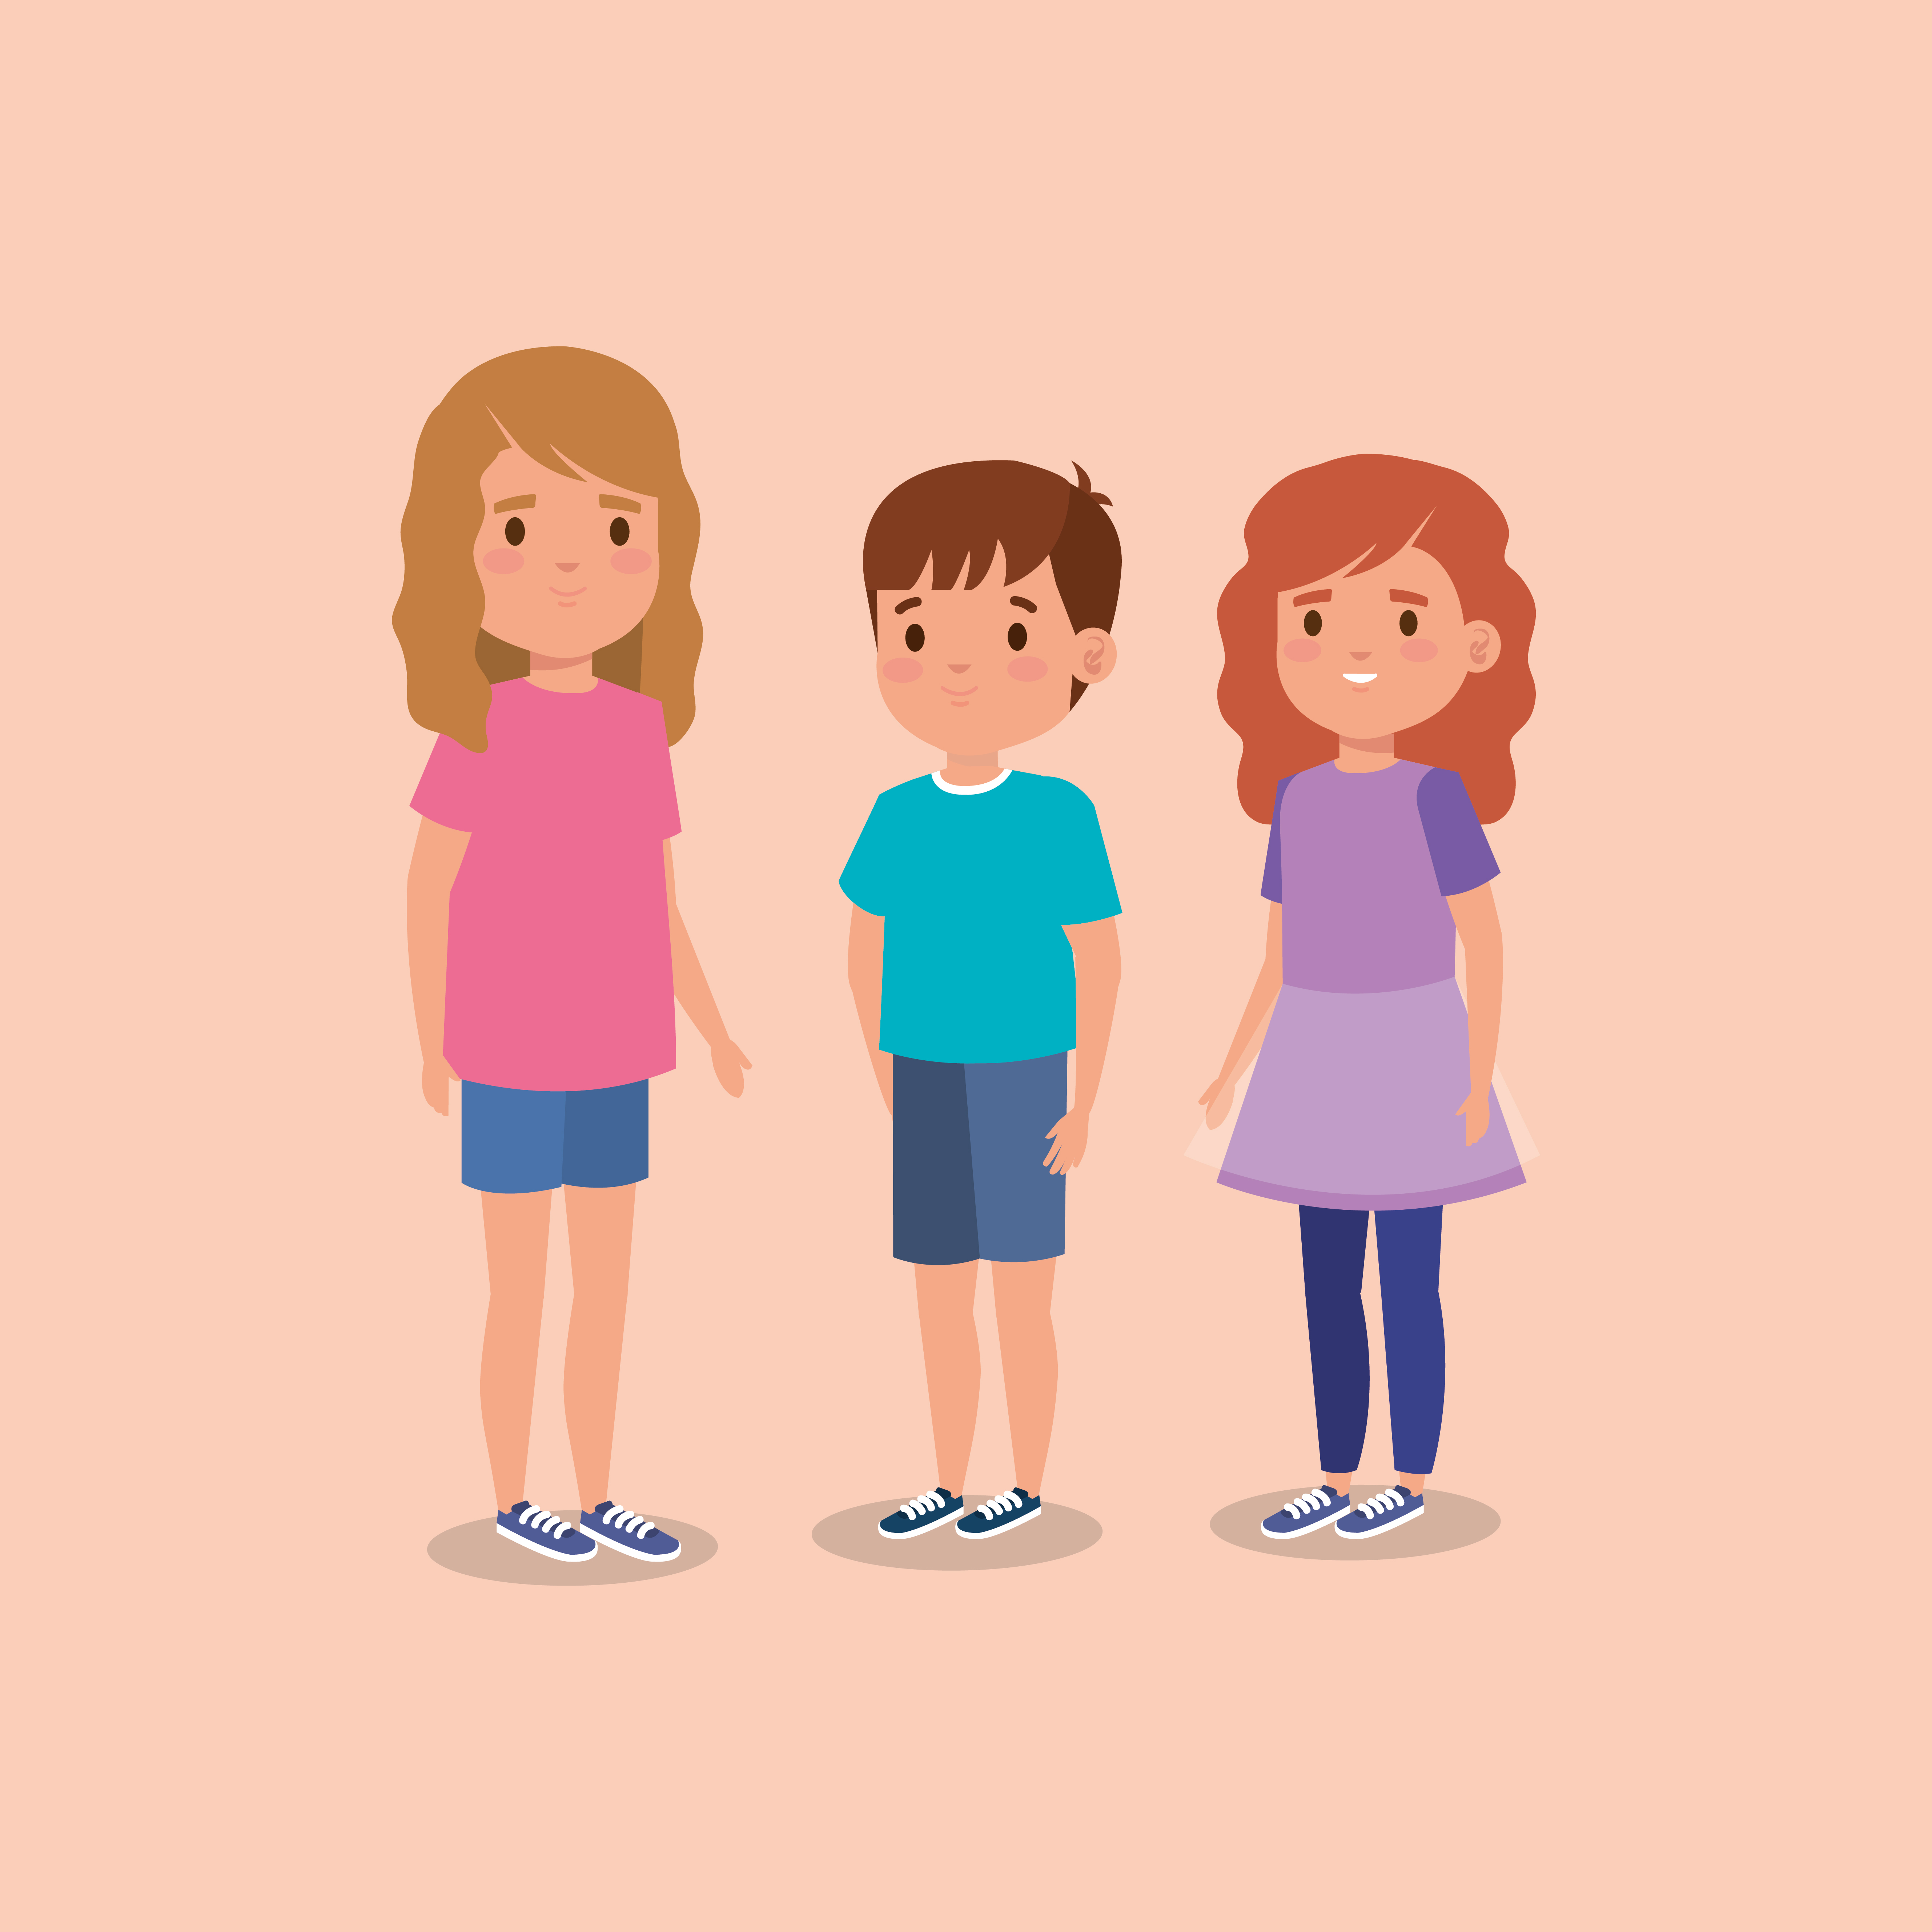
\includegraphics[width=.7\textwidth]{media/image24a.jpeg}
\end{center}

\reduline{A diferença entre a altura de Cláudia, a criança maior, e Lucas, a criança menor é dada pela expressão: 135 cm -- 120 cm = 25 cm.\hfill} 
\linhas{1}

\num{6} Inácio é barista. Ele trabalha em um restaurante e é responsável
por conhecer as preferência dos clientes e oferecer bebibas quentes. Entre elas, há uma muito consumida após as refeições no Brasil, o café. Para o preparo do café, é recomendado que a água apresente temperatura entre 93°C e 98°C. Sabe-se disso, porque a água é retirada do fogo antes de apresentar fervura, isto é, antes de atingir os 100°C, quando ela entra em ebulição. Utilize as informações do texto para responder aos itens a seguir.

\begin{center}
\includegraphics[width=.4\textwidth]{media/image24c.jpeg}
\end{center}

\begin{escolha}

\item Quais são as atividades de um barista?
\reduline{O barista é o profissional que trabalha em bares e restaurantes, responsável por conhecer as preferências dos clientes e oferecer bebidas quentes.\hfill}

\item Qual a temperatura ideal para passar o café?
\reduline{A água deve estar em temperatura entre 93°C e 98°C.\hfill} 
\linhas{2}

\item Qual o ponto de ebulição da água?
\reduline{A água entra em ebulição aos 100°C.\hfill} 
\linhas{1}
\end{escolha}
\pagebreak

\begin{comment}
\num{6} Roberta utiliza um termômetro profissional para medir a temperatura da
água que vai utilizar para fazer uma deliciosa receita de rosca
caseira. A receita diz que a temperatura da água deve ser exatamente 74ºC
para que possa ser adicionada. Em determinado momento, Roberta colocou
o termômetro na água e observou a seguinte temperatura: 63ºC. Podemos concluir que

\begin{escolha}
\item
  Roberta já pode adicionar a água à receita.
\item
  A água está mais quente do que o necessário; sendo assim, será
  necessário esfriar um pouco para que possa ser adicionada.
\item
  A água está 11ºC abaixo da temperatura ideal; sendo assim, ainda
  precisa aquecer um pouco.
\item
  Roberta não tem dados para analisar se adiciona ou não a água à receita.
\end{escolha}

\coment{Como a temperatura indicada no termômetro é de 63ºC e a temperatura
ideal para a receita é de 74ºC, a água ainda deverá ser aquecida em 11ºC.}
\end{comment}

\num{7} Observe as situações descritas a seguir e escreva o valor da massa (em quilogramas e em gramas) de cada item.

\begin{center}
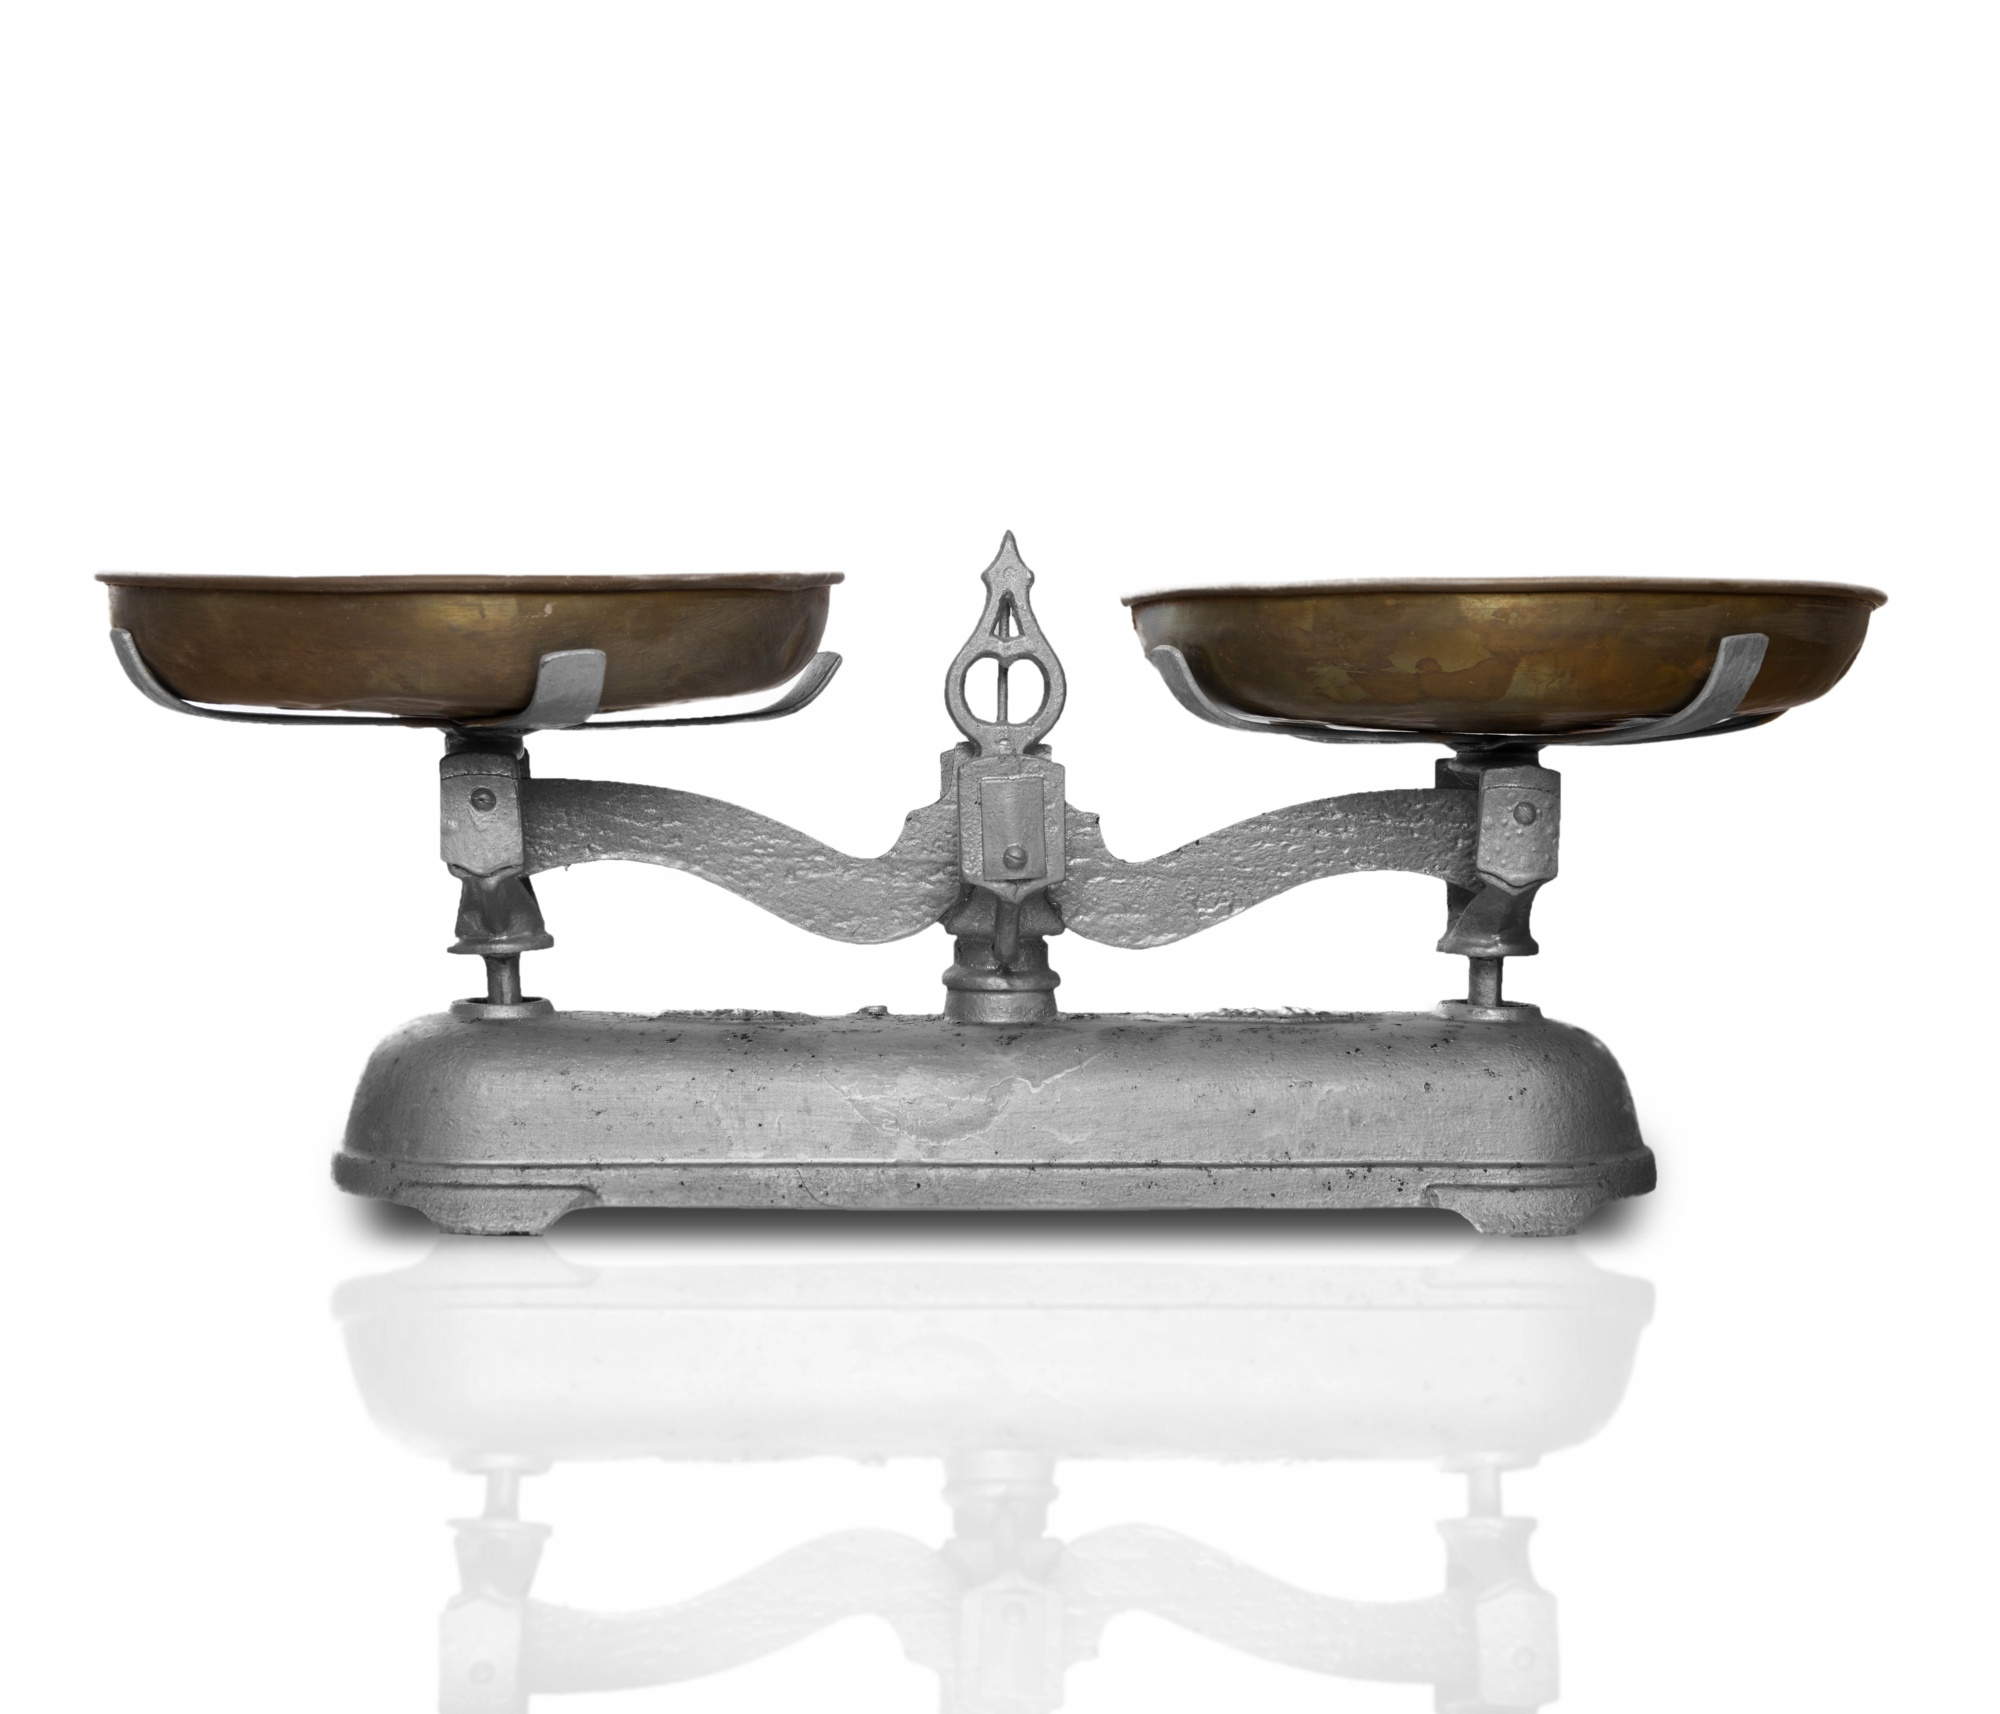
\includegraphics[width=.6\textwidth]{media/image24d.jpg}
\end{center}

\begin{escolha}
\item
  Para equilibrar os pratos de uma balança para pesar um saco de tomates, foram colocados um peso de 1 kg, outro de 500 g e outro de 100 g.
 \reduline{1,6 kg = 1.600 g.\hfill}
 \linhas{1}

\item
  Para equilibrar os pratos de uma balança para pesar um saco de batatas, foram colcoados um peso de 1 kg e outro de 500 g.
 \reduline{1,5 kg = 1.500 g.\hfill}
\linhas{1}

\item
  Para equilibrar os pratos de uma balança para pesar um saco de cenouras, foram colocados dois pesoas de 1 kg, um de 500 g, outro de 100 g e outro de 50 g.
 \reduline{2,65 kg = 2.650 g.\hfill}
\linhas{1}

\item
  Para equilibrar os pratos de uma balança para pesar um saco de cebolas, foram colocados um peso de 1 kg, dois pesos de 500 g, outro de 50 g e três outros de 10 g.
 \reduline{2,06 kg = 2.060 g.\hfill}
\end{escolha}

\num{8} Enquanto a mãe organizava a bolsa onde ficam termômetro e remédios, Carlos tomou o termômetro para medir a temperatura. O termômetro indicou que a temperatura 36,5°C. Sabendo que 37,5°C é o limite da temperatura sem febre, responda aos itens.

\begin{escolha} 
\item Qual o instrumento usado por Carlos para medir a temperatura?
\reduline{Carlos usou o termômetro para verificar a temperatura.\hfill}

\item Qual a temperatura de Carlos?
\reduline{A temperatura indicada pelo termômetro foi 36,5°C.\hfill}

\item A partir de qual temperatura, pode-se considerar que uma pessoa está com febre?
\reduline{A temperatura acima de 37,5°C pode ser considerada febril.\hfill}

\item Com base nas informações apresentadas, qual a avaliação se pode fazer da temperatura de Carlos?
\reduline{A temperatura de Carlos indica que ele está sem febre.\hfill} 
\end{escolha}


\num{9} Antonio acabou de se mudar e precisa colocar tela na janela para seu gato não fugir.
Ele não dispõe de régua, metro ou trena para medir a janela, mas sabe que seu palmo mede 22 centímetros. Ao medir a janela, verificou que a medida tem 9 palmos. Quantos centímetros mede a janela?

\reduline{A medida da janela que Antonio precisa colocar tela é dado pela expressão: 22 x 9 = 198 centímetros ou 1,98 m.\hfill}  
\linhas{1}

\num{10} Sarah usa 4 copos de água para preparar um pacote de gelatina. Sabendo que cada copo de água contem 250 ml. Quando qual a quantidade de água será necessária para fazer 8 pacotes?  

\reduline{Se Sarah usa 4 copos de 250 ml, o que equivale a 1 l de água, pois 250 x 4 = 1.000 ml ou 1 l, para preparar 8 pacotes serão necessários 8 l de água.\hfill} 
\linhas{1}

\begin{comment}
\num{8} Para a festa de aniversário de Arthur, seu pai encomendou 24 garrafas de
refrigerante. Dessas garrafas, 10 continham 3 litros (cada uma). Nas
demais garrafas, havia dois litros em cada uma. Com base nessas
informações responda ao que se pergunta a seguir.

\begin{escolha}
\item
  Qual é a quantidade de refrigerante, em mililitros, encomendada pelo pai de Arthur?
\item\reduline{(10 x 3) + (14 x 2) = 30 + 28 = 58 L = 58 000 mL.\hfill}

\item
  Se cada convidado da festa consumiu exatamente 400 mililitros de refrigerante e
  todo o refrigerante foi consumido durante a festa, quantas pessoas
  foram ao aniversário de Arthur?
\item \reduline{58.000 : 400 = 145 pessoas compareceram à festa.\hfill}
\end{escolha}

\num{10} Ana Luísa deve tomar um remédio de 8 em 8 horas. Se ela tomou o primeiro
comprimido às 6 horas da manhã, qual será o horário em que ela deverá tomar
o terceiro comprimido?

\begin{mdframed}[linewidth=2pt,linecolor=salmao,roundcorner=2pt]
\coment{Primeiro comprimido: 6 horas da manhã.}

\coment{Segundo comprimido: 6 + 8 = 2 horas da tarde ou 14 horas.}

\coment{Terceiro comprimido: 14 + 8 = 22 horas ou 10 horas da noite.}
\end{mdframed}
\end{comment}

%REPETIDOS 1
\section*{Treino}

\num{1} Samanta estuda um colégio integral cujos horários de aula são:  

\begin{longtable}[]{@{}lll@{}}
\toprule
& \textbf{Entrada} & \textbf{Saída}\tabularnewline
\midrule
\endhead
\textbf{Manhã} & 7h00 & ?\tabularnewline
\textbf{Tarde} & 14h00 & 18h00\tabularnewline
\bottomrule
\end{longtable}

\begin{center}
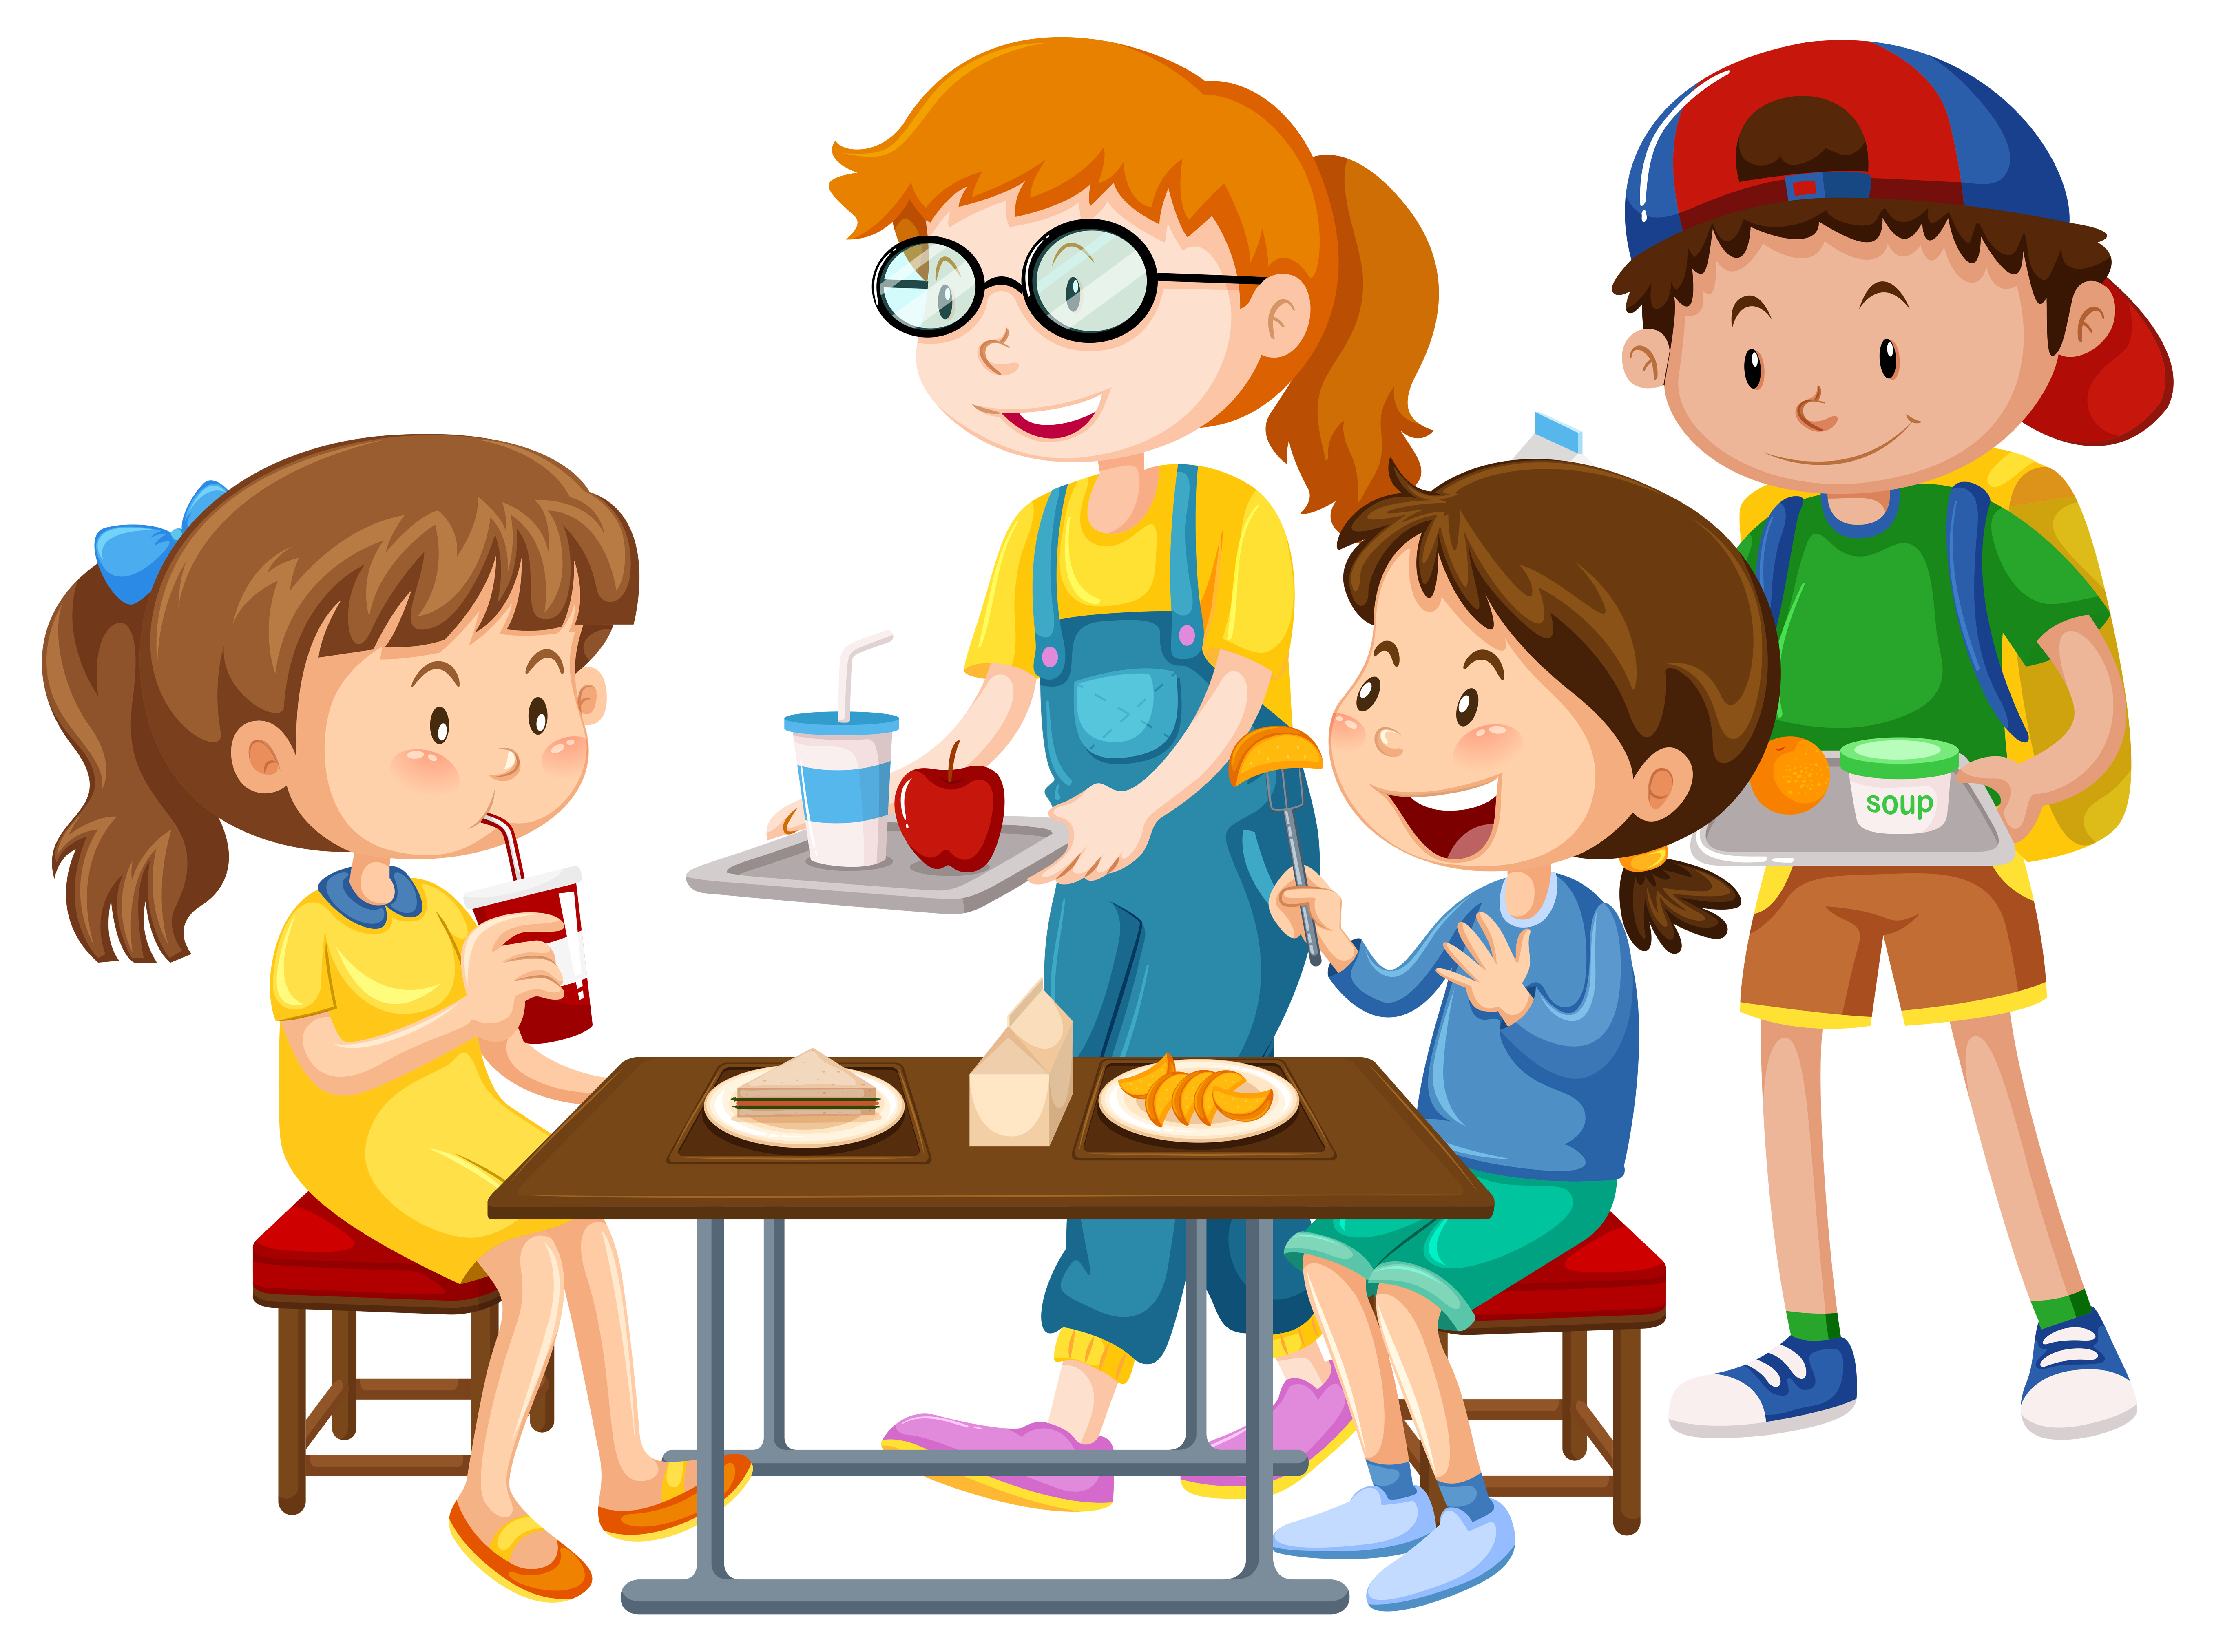
\includegraphics[width=.4\textwidth]{media/image24e.jpeg}
\end{center}

No período da manhã, Samanta permanece durante 5 horas e 30 minutos em sala de aula. 
E, no período da tarde, realiza atividades complementares.
Em que horário começa o almoço de Samanta?

\begin{multicols}{2}
\begin{escolha}
\item
  11:00.
\item
  11:30.
\item
  12:00.
\item
  12:30.
\end{escolha}
\end{multicols}

\num{2} Na receita, a médica orienta Marcela a tomar o xarope 4 vezes ao
dia durante 15 dias. Sabendo que a dose é de 8 mL e que o frasco do remédio
contém 100 mL, quantas unidades do remédio serão necessárias para concluir o 
tratamento? 

\begin{multicols}{2}
\begin{escolha}
\item
  2.
\item
  3.
\item
  4.
\item
  5.
\end{escolha}
\end{multicols}

\num{3} Bárbara teve de fazer uma viagem para fechar um grande negócio. Se o voo
saiu do aeroporto às 10 horas e 42 minutos e chegou ao destino às 14
horas e 8 minutos, qual foi o tempo de duração do voo?

\begin{multicols}{2}
\begin{escolha}
\item
  11.760 segundos.
\item
  9.542 segundos.
\item
  5.364 segundos.
\item
  2.500 segundos.
\end{escolha}
\end{multicols}

\chapter{Unidades e medidas}
\markboth{Módulo 5}{}

\section*{Habilidades do SAEB}

\begin{itemize}
\item Medir ou comparar perímetro ou área de figuras planas desenhadas em
malha quadriculada.
\item Identificar horas em relógios analógicos ou associar horas em relógios
analógicos e digitais.
\item Resolver problemas que envolvam perímetro de figuras planas.
\item Resolver problemas que envolvam área de figuras planas.
\end{itemize}

\subsection{Habilidades da BNCC}

\begin{itemize}
\item EF04MA21, EF04MA22.
\end{itemize}

\conteudo{
\textbf{Ampliação e redução de uma figura plana}\bigskip

Ampliação é o processo que realizamos quando queremos aumentar algo,
como, por exemplo, figuras planas, sem alterar suas características.

A figura menor a seguir teve o tamanho de todos os seus lados. 
Observe, no entanto, que as características foram mantidas.

%Fazer a figura a seguir sem marcar os ângulos e a primeira deve ter lado
%3 cm e a segunda lado 6 cm.

\begin{center}
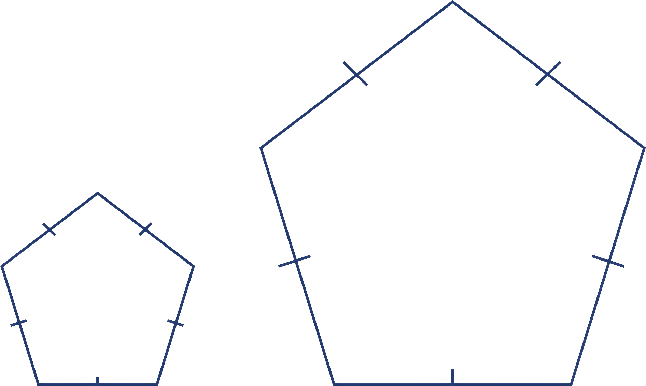
\includegraphics[width=.7\textwidth]{media/image25.png}
\end{center}

Redução é o processo que realizamos quando queremos diminuir algo,
como, por exemplo, figuras planas, sem alterar suas características.

A figura maior a seguir teve o tamanho de todos os seus 
lados dividido por dois, mas observe que foram mantidas as
mesmas características.

%Fazer a figura a seguir sem marcar os ângulos e a primeira deve ter lado
%6 cm e a segunda lado 3 cm.

\begin{center}
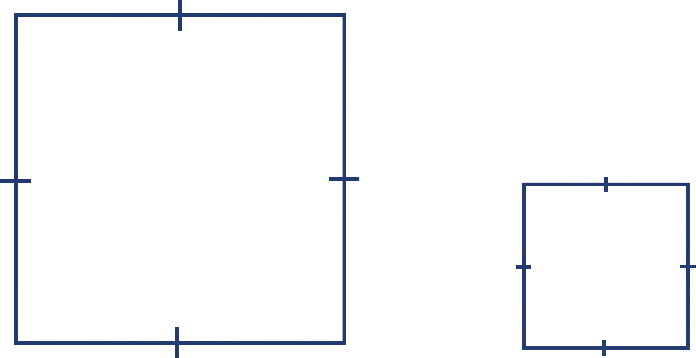
\includegraphics[width=.7\textwidth]{media/image26.png}
\end{center}

Muitas vezes, recorremos a malhas quadriculadas para 
realizar aumento ou redução. Com isso, é possível comparar áreas de
superfícies e até ter certeza de alguma ampliação ou alguma redução.\bigskip

\textbf{O relógio: as horas e os minutos}\bigskip

Um instrumento muito usado para medir o tempo é o relógio de ponteiros. 
Ele também é chamado de \textbf{relógio análogico}, cujo nome se deve 
ao modo de seu mecanismo que é movido à corda. 
Hoje, com o desenvolvimento das tecnologias, é mais comum encontrar no cotidiano 
relógios digitais, com mecanismo alimentados por bateria.  

Nos relógios analógicos, a área do mostrador é dividida em doze partes iguais, 
numeradas de 1 a 12. Em geral, esse relógio apresenta três ponteiros:
o menor, o das horas, que é também o mais lento dos três; o médio, dos minutos; 
e o mais longo e mais fino, dos segundos, o ponteiro mais rápido. 

As horas estão representados pelos números de 1 a 12, 
sendo 12 comumente chamado de meio-dia ou meia-noite. 

Nos intervalos dos números que representam as horas, há pequenos traços verticais
que representam os minutos. A cada intervalo entre um número e outro, há cinco tracinhos
que representam 5 minutos. Uma volta completa do ponteiro médio
representa 60 minutos ou 1 hora.

O ponteiro maior indica os segundos, e a cada 60 segundos forma-se 1 minuto.
}

\pagebreak
\section*{Atividades} 

\num{1} Escreva por extenso as horas representadas a seguir. Depois, ao lado, registre uma atividade que você costuma fazer em cada um desses horários.

\begin{figure}[htpb!]
\centering
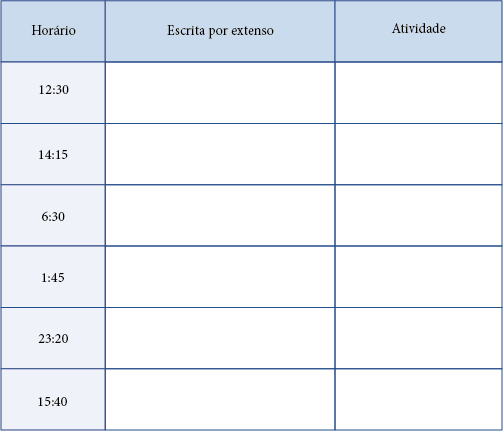
\includegraphics[width=\textwidth]{media/image28.png}
\end{figure}

\num{2} Escreva no espaço correspondente quantos meses compõem um período de:

\begin{escolha}
\item
  2 anos:\reduline{24 meses\hfill}

\item
  8 anos:\reduline{96 meses\hfill}

\item
  1 década:\reduline{120 meses\hfill}

\item
  1 século:\reduline{1.200 meses\hfill}
\end{escolha}


\num{3} Observe atentamente as figuras e responda aos itens, considerando que todos os quadradinhos têm a mesma área.

\begin{figure}[htpb!]
\centering
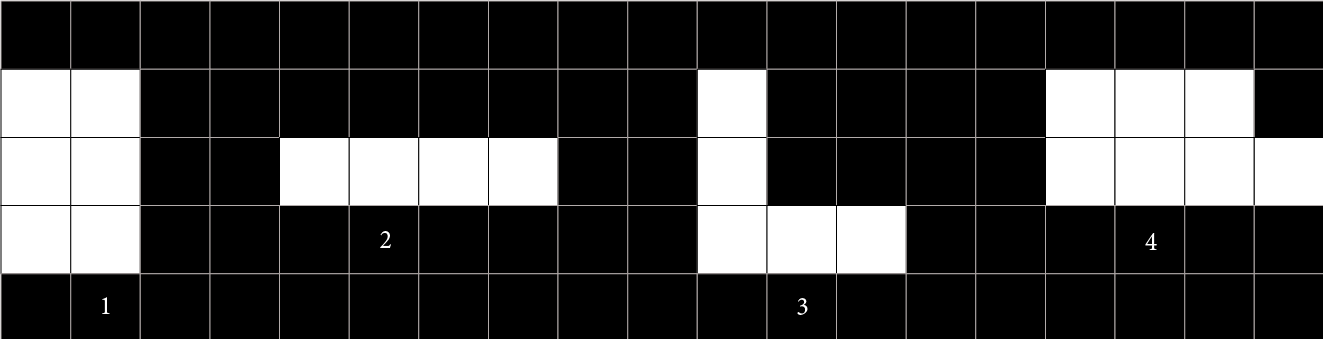
\includegraphics[width=\textwidth]{media/image31.png}
\end{figure}

\begin{escolha}
\item Qual figura apresenta a maior área?
\reduline{A figura que apresenta a maior área é a figura 4.\hfill}

\item Qual figura apresenta menor área? 
\reduline{A figura que apresenta a menor área é a figura 2.\hfill}
\end{escolha}

%A figura 1 é composta de 6 quadradinhos. A figura 2 é composta de 4 quadradinhos. A figura 3 é composta de 5 quadradinhos. A figura 4 é composta de 7 quadradinhos. Como os quadradinhos são de mesmo tamanho, pode-se concluir que a figura que possui a menor área é a figura 2, por ser composta de um número menor de quadradinhos.

\num{4} Os desenhos a seguir representam as plantas baixas, inicial
e final, e o formato da área de uma praça construída em um condomínio. 

\begin{figure}[htpb!]
\centering
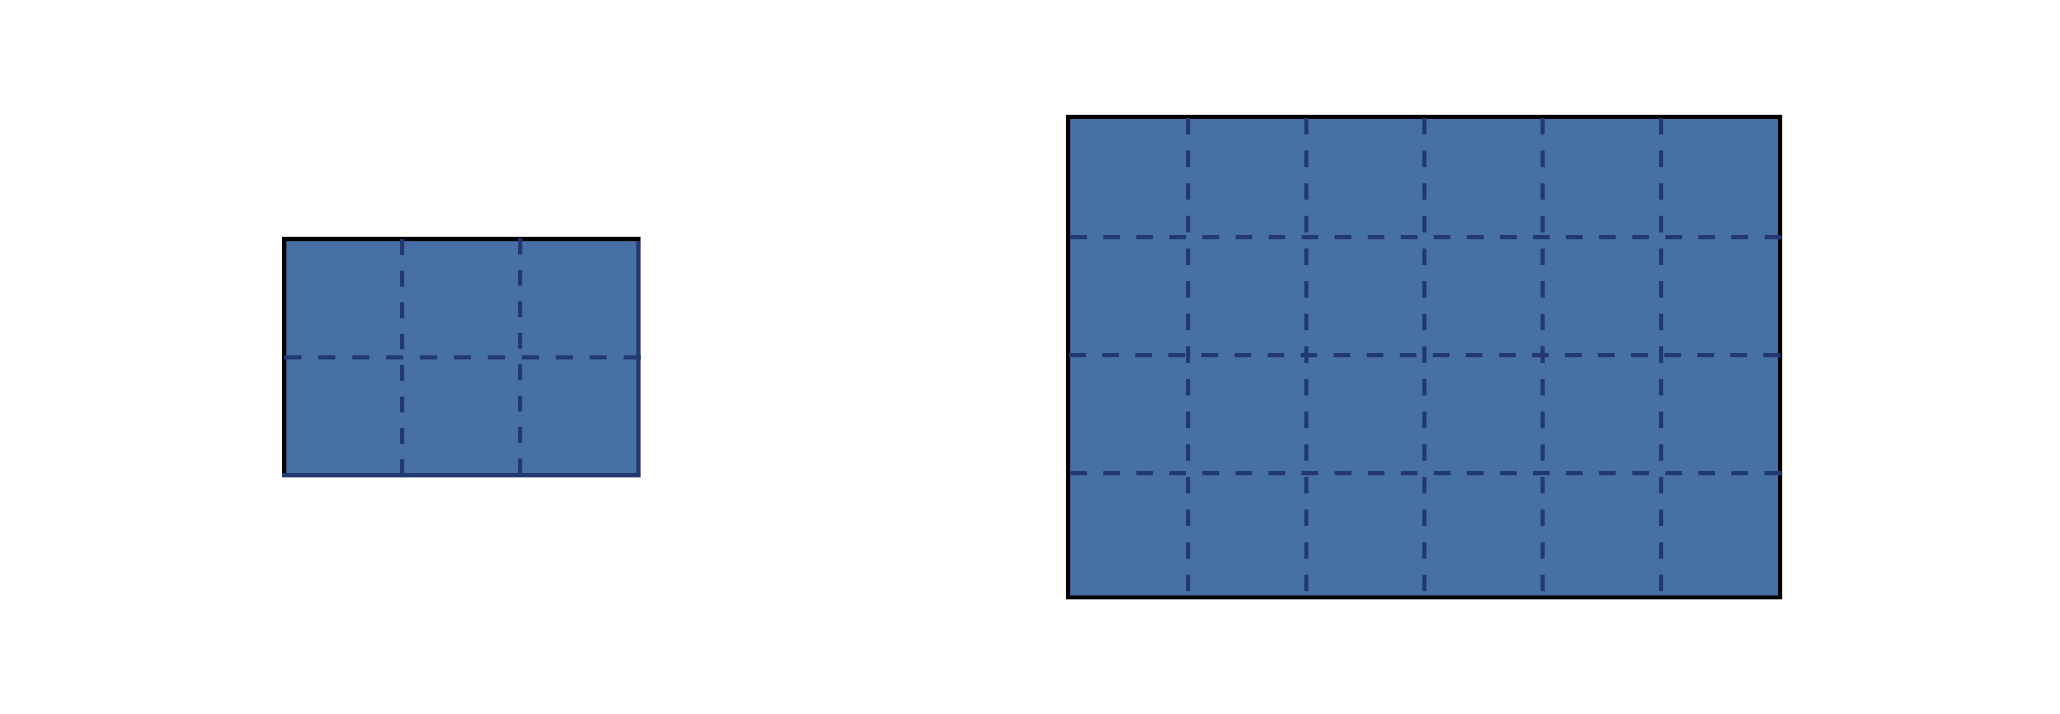
\includegraphics[width=\textwidth]{media/image30.png}
\end{figure}

A área prevista no primeiro projeto é diferente daquela do projeto final.
O aumento da área foi possível graças à incorporação de um terreno ao lado.

Com base nas duas plantas, quantas vezes a área final é maior que a inicial?

\reduline{O projeto incial ocupa 6 unidades de área; e o projeto final, 24 unidades. Portanto,  a área do projeto final é 4 vezes maior que o do inicial.\hfill}

%A praça menor teria 6 quadradinhos preenchendo sua área, enquanto a grande terá 24 quadradinhos. Sendo assim, a área da praça maior é quatro vezes a área da praça menor.
\pagebreak

\num{5} Um arquiteto fez um primeiro esboço de uma construção no formato de cruz
que teria de executar.

\begin{figure}[htpb!]
\centering
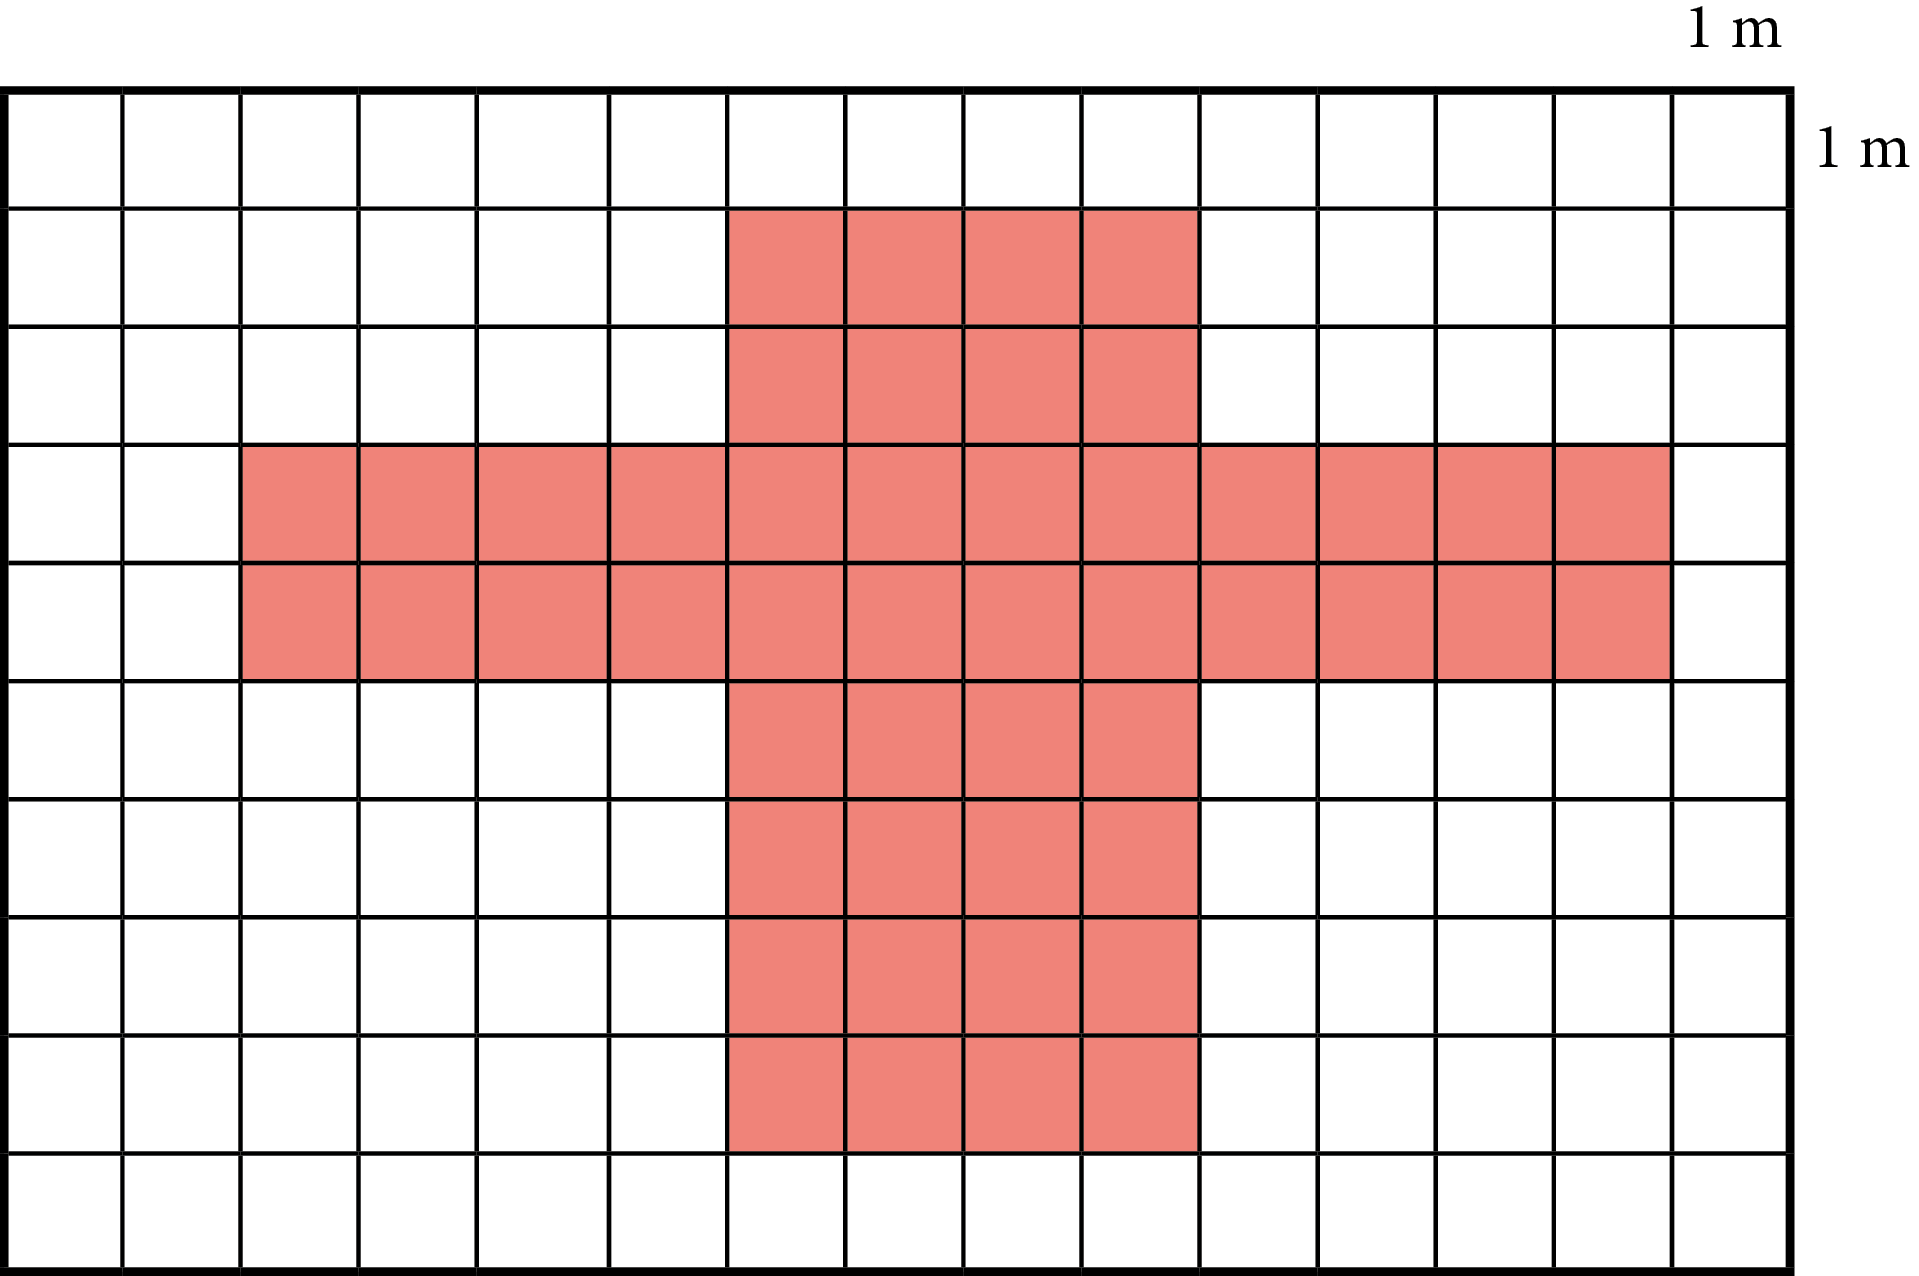
\includegraphics[width=\textwidth]{media/image32.png}
\end{figure}

No projeto final, todos os lados foram reduzidos à metade. Desenhe a nova imagem do projeto.

\begin{mdframed}[linewidth=2pt,linecolor=salmao,roundcorner=2pt]
\vspace{7cm}
\end{mdframed}
\pagebreak

\num{6} Na malha quadriculada a seguir, cada quadrado representa uma área de 17
metros quadrados.

\begin{figure}[htpb!]
\centering
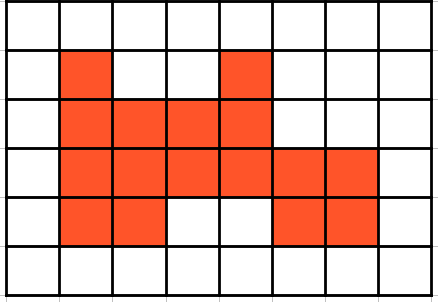
\includegraphics[width=.7\textwidth]{media/image33_.png}
\end{figure}

Qual é a área da malha quadriculada que a figura destacada ocupa?

\reduline{Realizando-se a contagem de quadradinhos que preenchem a figura, chega-se
ao número 16. Portanto: 16 x 17 = 320 metros quadrados.}

\num{7} No próximo domingo, Sandro participará de uma corrida de bicicletas.
Para concluir a prova, ele deve realizar 17 voltas. Sabendo que o circuito tem um formato
retangular com 50 metros no lado maior e 30 de metros no lado menor, qual é distância aproximada em quilômetros ele percorrerá ao concluir a prova?

\reduline{Após concluir a prova, Sandro terá percorrido (2 x 50) + (2 x 30) x 17 = 2.720 metros. Então, Sandro percorrerá quase 3 km.\hfill}

\num{8} Ajude a abelha a chegar na colmeia, pintando 16 espaços.

\begin{figure}[htpb!]
\centering
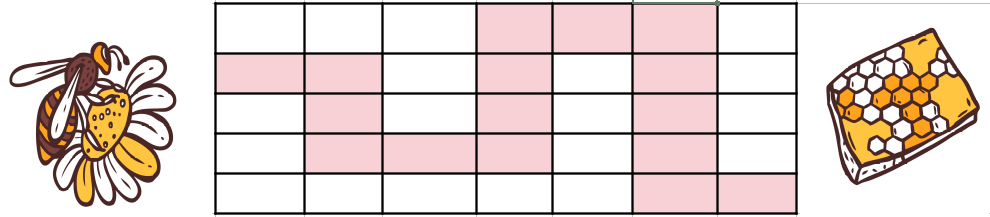
\includegraphics[width=\textwidth]{media/image33a.png}
\end{figure}  


\num{9} Cláudia decidiu trocar o piso do banheiro do filho e desenhar com ladrilhos 
a inicial do nome de Artur. Se cada ladrilho tiver dimensão de dois metros quadrados 
qual área a letra A deve ocupar no banheiro do filho?

\begin{figure}[htpb!]
\centering

\includegraphics[width=.3\textwidth]{media/image29.png}
\end{figure}

\reduline{O total da área é dado pela expressão 14 quadradinhos x 2 metros quadrados = 28 metros quadrados.\hfill}
\linhas{1}


\num{10} Júlia encontrou uma malha quadriculada com as seguintes letras.

\begin{figure}[htpb!]
\centering
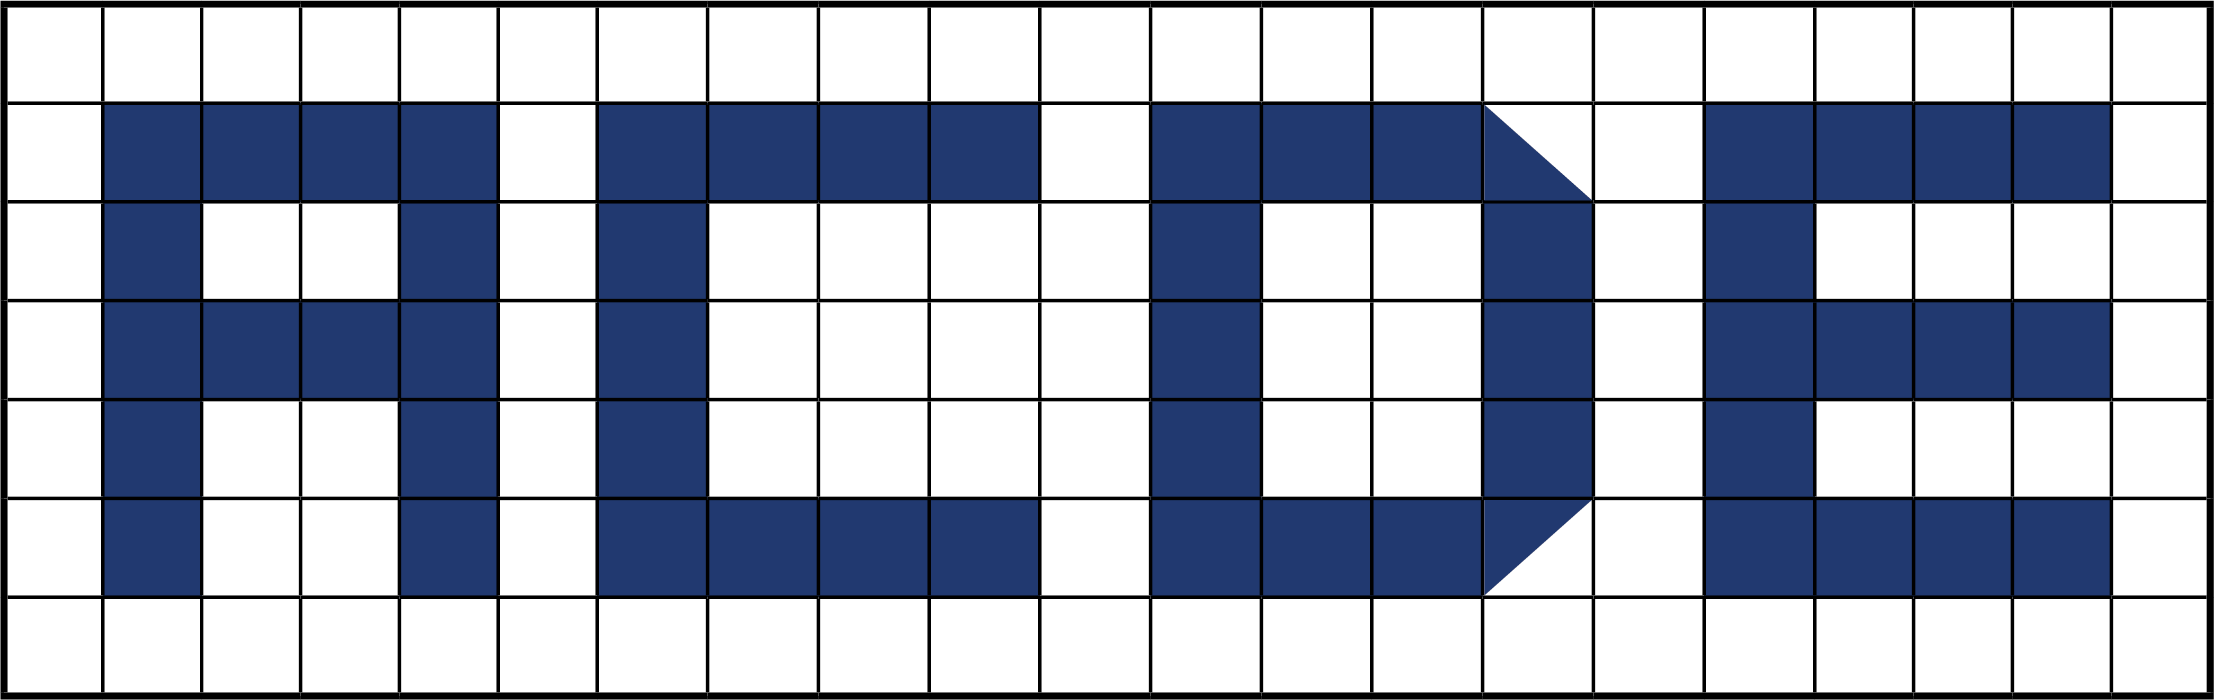
\includegraphics[width=.6\textwidth]{media/image34.png}
\end{figure}

\begin{escolha}
\item Ajude Júlia a encontrar as duas letras que ocupam a mesma área. 
\reduline{As duas letras que ocupam a mesma área são A e E. Cada uma dela ocupam 14 quadrados.\hfill}
\linhas{1} 

\item Supondo que a área de cada quadrado é igual a 1 metro quadrado, 
quantos metros quadrados ocupam as duas letras juntas?
\reduline{Se cada uma das letras A e E ocupam individualmente 14 quadrados e cada quadrado é igual a 1 metro quadrado. Então 14 x 2 = 28 metros quadrados.} 
\linhas{1}

%Letra A: 14 quadradinhos.
%Letra C: 11 quadradinhos.
%Letra D: 13 quadradinhos.
%Letra E: 14 quadradinhos.
%As duas letras que ocupam asuperfícies de mesmo tamanho são a A e a E.
\end{escolha}

\begin{comment}
\num{10} Inês tem um compromisso inadiável às 20h25. Desenhe um relógio analógico
com os ponteiros indicando a hora do compromisso de Inês.

\begin{mdframed}[linewidth=2pt,linecolor=salmao,roundcorner=2pt]
\coment{O ponteiro das horas deve estar um pouco depois do número 8, e o ponteiro dos minutos deve estar apontando diretamente o número 5.}
\vspace{11cm}
\end{mdframed}
\end{comment}

\pagebreak
\section*{Treino}

\num{1} Luigi tem três anos e meio. Qual a idade de Luigi em meses?

\begin{multicols}{2}
\begin{escolha}
\item 24 meses. 

\item 36 meses.

\item 42 meses. 

\item 48 meses.
\end{escolha}
\end{multicols}


\num{2} Observe atentamente as figuras abaixo:

\begin{figure}[htpb!]
\centering
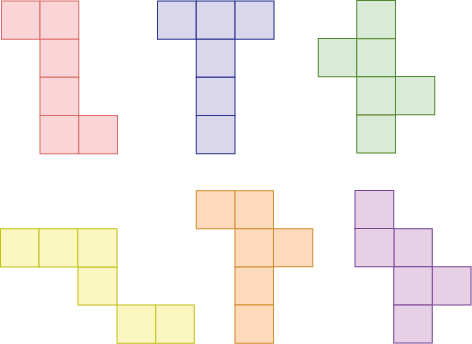
\includegraphics[width=.7\textwidth]{media/image36.png}
\end{figure}

Após a análise das figuras, percebe-se que:

\begin{escolha}
\item
  a primeira figura é a que possui a maior área.
\item
  a última figura é a que possui a menor área.
\item
  todas as figuras possuem a mesma área.
\item
  todas as figuras possuem áreas diferentes.
\end{escolha}


\begin{comment}
\num{1} Paulo resolveu ir a uma exposição. Observe o mapa, em que cada quadradinho tem um lado que representa 2 metros na realidade.

\begin{figure}[htpb!]
\centering

\includegraphics[width=\textwidth]{media/image35.png}
\end{figure}

O caminho indicado é o de um corredor entre a bilheteria e o início da exposição.
Quanto ele precisará andar para chegar?

\begin{escolha}
\item
  8 m.
\item
  10 m.
\item
  12 m.
\item
  14 m.
\end{escolha}

\pagebreak
\end{comment}


\num{3} Heloísa estuda no período da tarde. Ela começa a se arrumar para ir à escola 
quando o ponteiro menor está entre o 11 e o 12 e o ponteiro médio sobre o sete. Ontem,
ela ficou pronta em 55 minutos. Que horário o relógio mostrava quando ela ficou pronta?

\begin{comment} 

Maria começou a se arrumar para um passeio com suas amigas na hora em
que, no relógio de seu quarto, o ponteiro menor estava entre o 11 e 12, enquanto o ponteiro maior estava sobre o 7. Ela terminou de se arrumar em 55 minutos. Que horário
o relógio estava marcando nesse segundo momento?
\end{comment}

\begin{multicols}{2}
\begin{escolha}
\item
  11 horas e 50 minutos.
\item
  12 horas.
\item
  12 horas e 20 minutos.
\item
  12 horas e 30 minutos.
\end{escolha}
\end{multicols}


\chapter{O sistema monetário brasileiro}
\markboth{Módulo 6}{}

\section*{Habilidades do SAEB}

\begin{itemize}
\item Relacionar valores de moedas e/ou cédulas do sistema monetário
brasileiro, com base nas imagens desses objetos.

\item Resolver problemas que envolvam moedas e/ou cédulas do sistema
monetário brasileiro.
\end{itemize}

\subsection{Habilidade da BNCC}

\begin{itemize}
  \item EF04MA25.
\end{itemize}

\pagebreak
\conteudo{
\textbf{Real: moeda brasileira} 

A moeda usada no Brasil é o Real. Na escrita, a forma de representação é 
\textbf{R\$} ao lado do valor. Por exemplo, R\$ 1,00 (um real), R\$ 5,00 (cinco reais),
R\$ 10 (dez reais), R\$ 50,00 (cinquenta reais).  Por meio dessa moeda, se estabelecem
relações comerciais, como a compra de um doce, de uma aparelho de televisão ou carro.
Assim, são vendidos e comprados produtos e serviços. Aquele que adquire um bem 
ou um serviço é chamado de \textbf{consumidor} e aquele que vende produtos pode ser o 
\textbf{vendedor ou comerciante} e quem fornece serviços é o \textbf{prestador de serviço}, como encanador, taxista, médico, advogado, por exemplo.

Veja, a seguir, as representações das cédulas e das moedas em vigor.

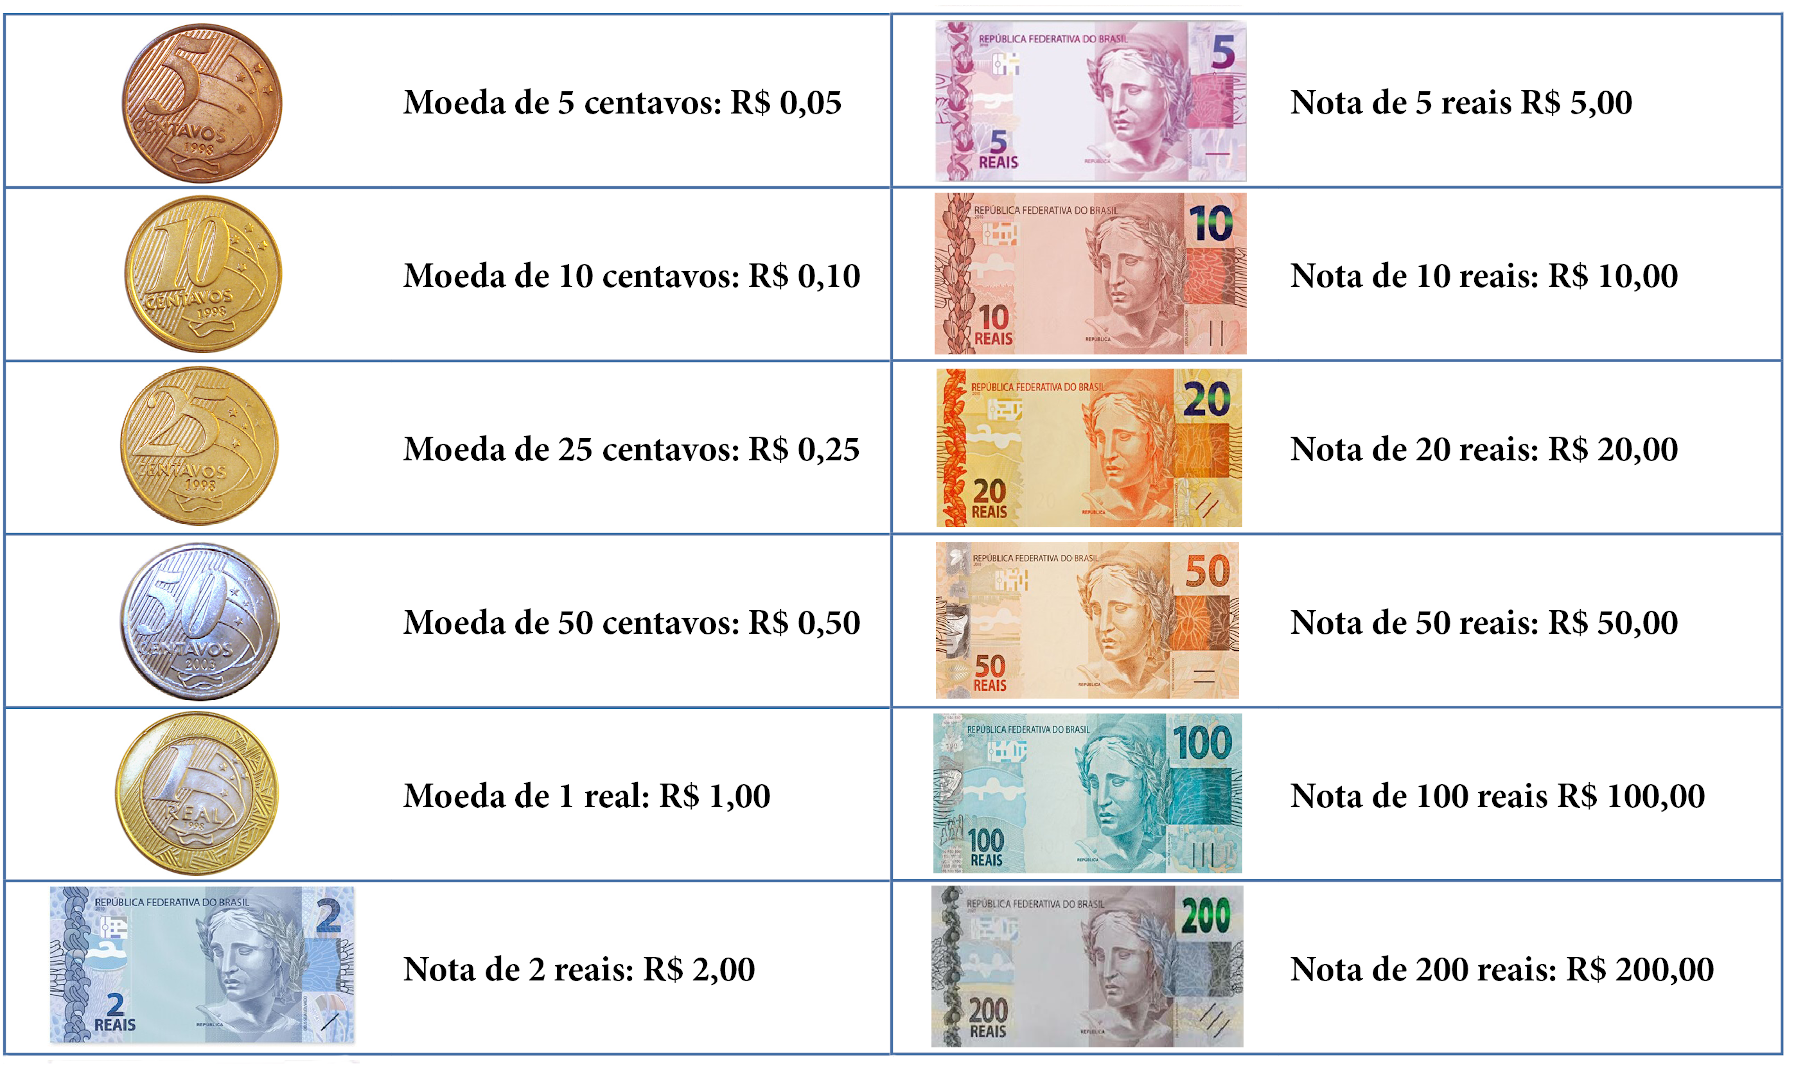
\includegraphics[width=\textwidth]{media/image37.png}
}

\section*{Atividades}


\num{1} Componha o total, utilizando, em cada caso, o maior número possível de cédulas de cada valor.

\begin{escolha}
\item Com cédulas de 20, 10 e 2 reais, como se pode compor o valor R\$ 836,00?
\reduline{Quarenta e uma cédulas de 20 reais, uma cédula de 20 reais e três cédulas de 2 reais.\hfill}

\item Com cédulas de 200, 50 e 20 reais, como se pode compor o valor R\$ 3.940?
\reduline{Dezenove cédulas de 200 reais, duas cédulas de 50 reais e duas cédulas de 20 reais.\hfill}

\item Com cédulas de 100, 10 e 5 reais, como se pode compor o valor R\$ 1.735?
\reduline{Dezessete cédulas de 100 reais, três cédulas de 10 reais e uma cédula de 5 reais.\hfill}
\end{escolha}


\num{2} Alice foi ao açougue e comprou dois quilos de contra-filé
a R\$ 54,50 o quilo. Sabendo que ela pagou com uma nota de R\$ 100,00 
e outra de R\$ 20,00. Quais cédulas e moedas ela recebeu de troco?

\reduline{54,50 x 2 -- 120 = 11. Os alunos podem compor como quiserem 
o valor em notas e moedas. Uma possibilidade de resposta é: Alice recebeu
duas notas de R\$ 5,00 e duas moedas de R\$ 0,50.}

\num{3} Heitor economizou para comprar um jogo de montar no valor de R\$ 120,00.
Quando chegou à loja, soube que o brinquedo estava em promoção, com desconto de R\$ 11,50. Quanto Heitor pagou pelo produto?

\begin{center}
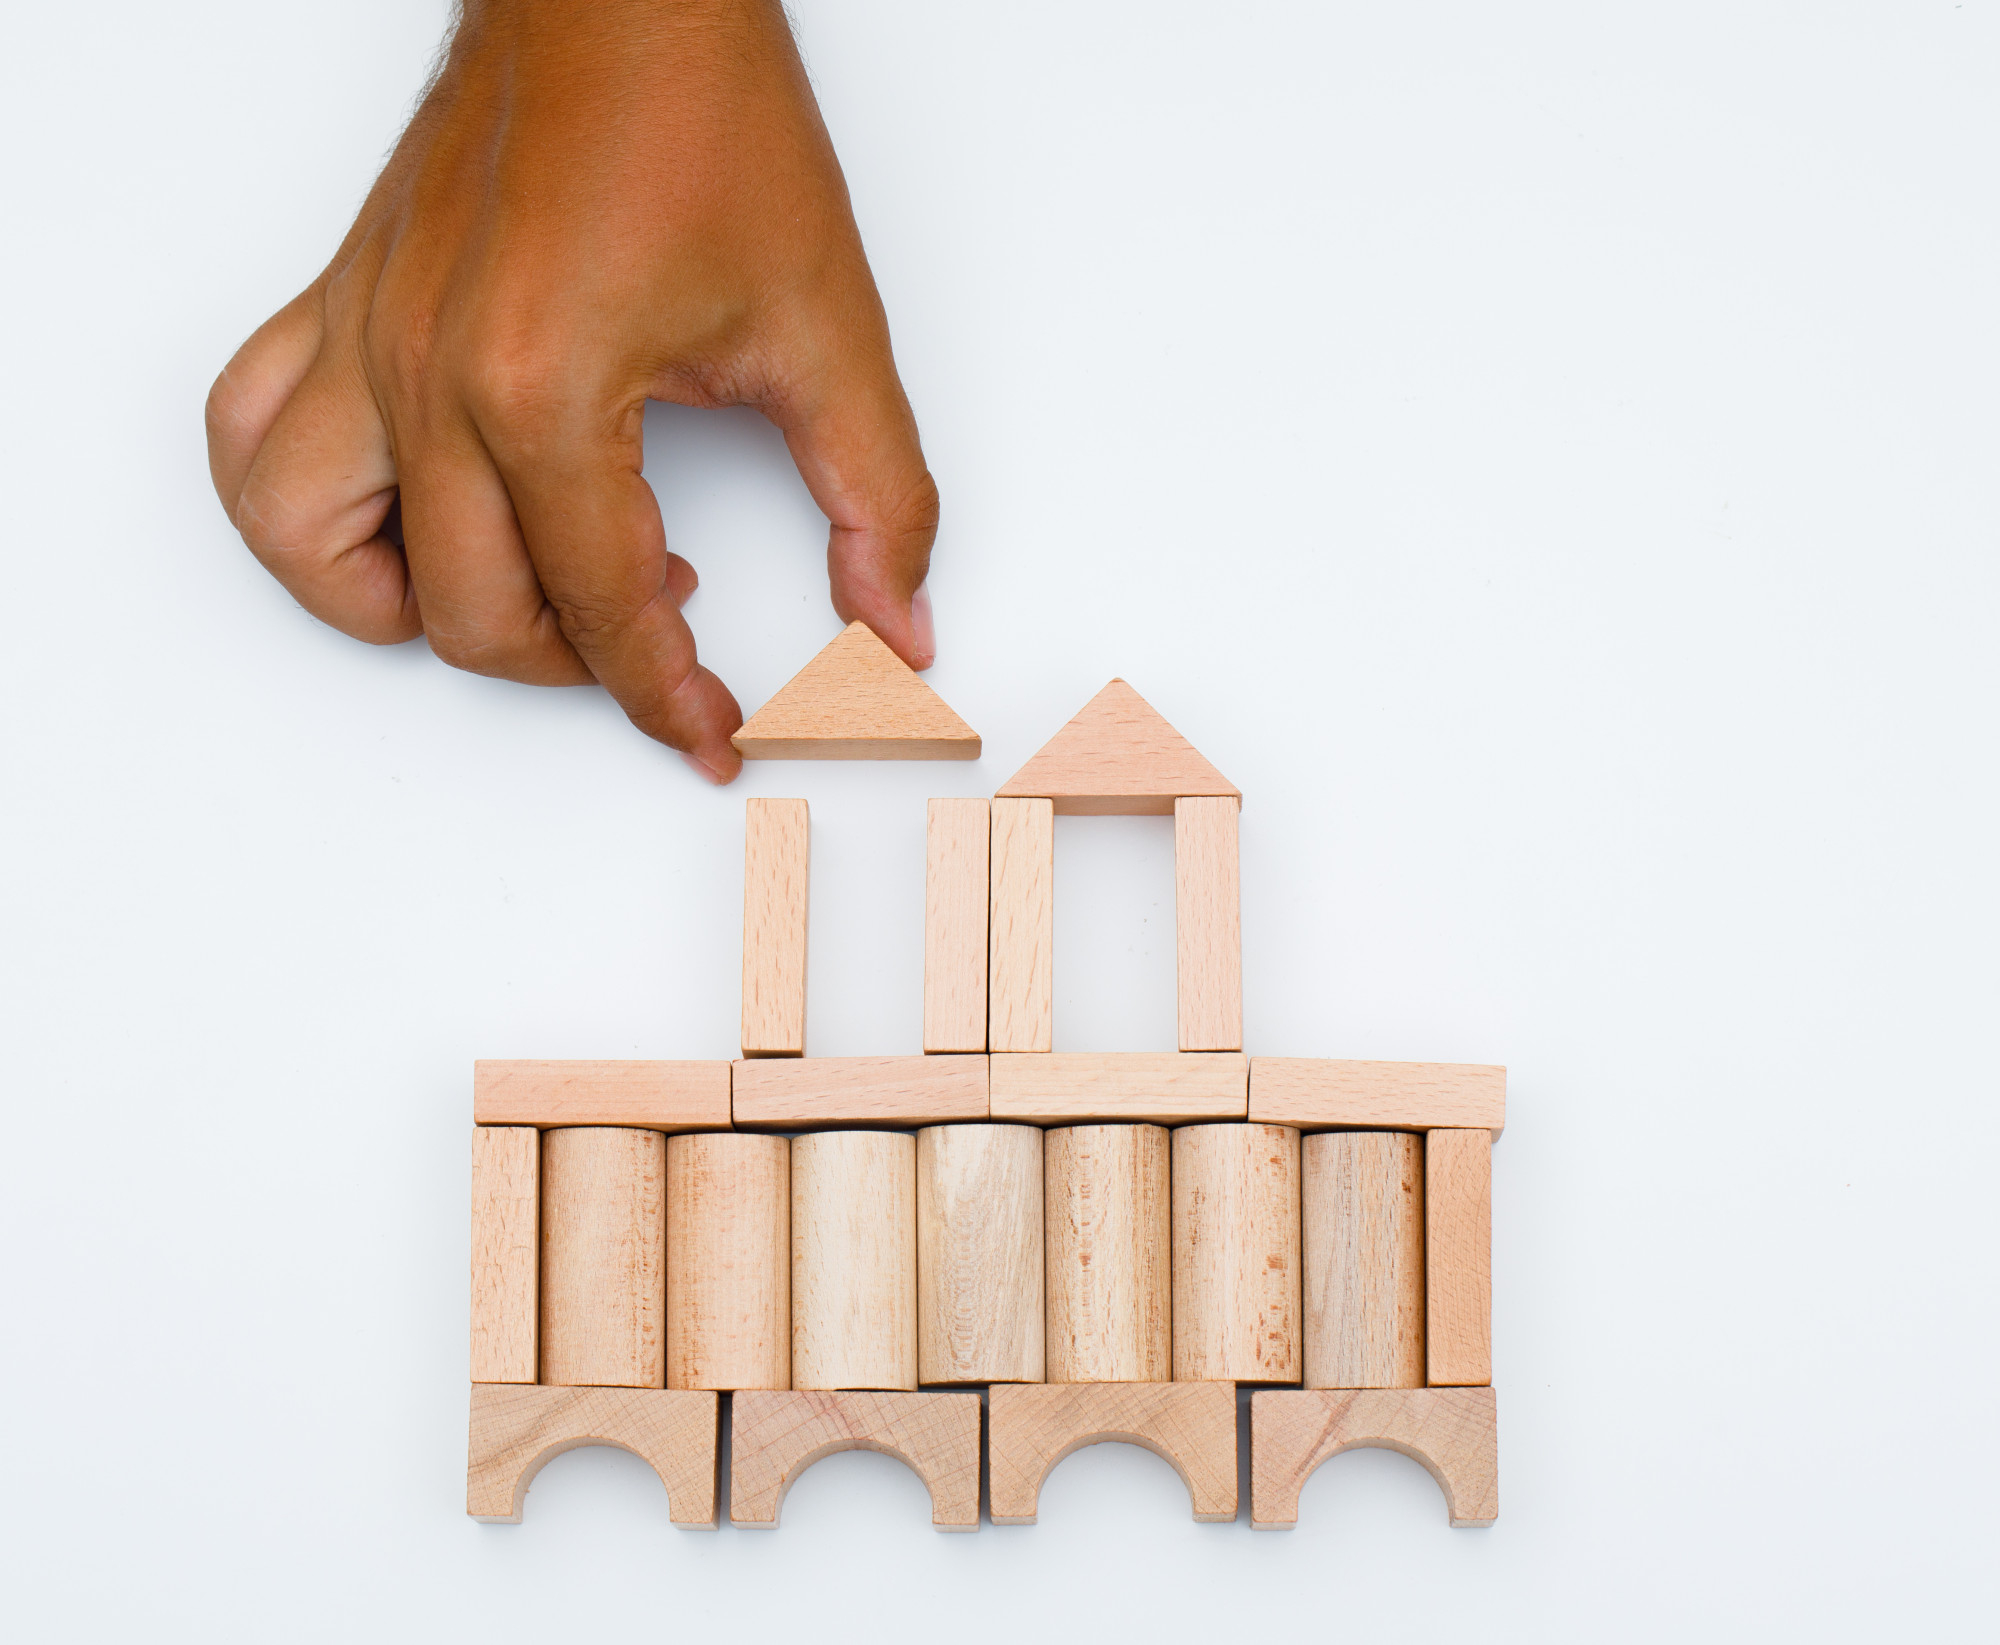
\includegraphics[width=.5\textwidth]{media/image37a.jpg}
\end{center}

\reduline{Heitor pagou pelo produto 120 -- 11,50 = 108,50.\hfill}

\begin{comment}
Marta foi à papelaria comprar uma caneta de que estava precisando para
continuar seus estudos. Ela comprou uma caneta que custava 7 reais e 25
centavos. Sabendo-se que ela pagou com uma nota de 10 reais, quais
cédulas e moedas ela recebeu de troco?

\reduline{Possibilidade de resposta: uma cédula de 2 reais, uma moeda de 50 centavos e uma moeda de 25 centavos.\hfill}
\linhas{2}

\num{2} Caíque economizou muito dinheiro, pois queria comprar um \textit{videogame} usado,
que custava R\$ 2.490,00 à vista. Ele conversou com o vendedor e pediu
um desconto extra e foi atendido com um desconto de R\$ 250,00. Quanto
ele pagou pelo \textit{videogame}?

\reduline{R\$ 2.490,00 -- R\$ 250,00 = R\$ 2.240,00.\hfill}
\linhas{2}
\end{comment}


\num{4} Susan tem R\$ 4.000,00 de saldo na conta do bancária e tem de pagar as contas a seguir: 

\conteudo{
\textbf{  \item Cartão de crédito: R\$ 1.128,00;
  \item Aluguel: R\$ 1.900,00;
  \item \textit{Petshop}: R\$ 480,00;
  \item Clube de assinatura: R\$ 635,00.
}}

Ela terá dinheiro suficiente para pagar todas as contas? Explique.

\reduline{Ana tem 1.128 + 1.900 + 480 + 635 = 4.143 reais de contas para pagar, mas só tem R\$ 4.000,00 na conta do banco, valor das contas que é 143 reais menor do que o valor de ela precisa.\hfill}
\linhas{1}

\num{5} Marcela comprou um carro pelo preço de R\$ 60.000,00.
O valor foi parcelado em 24 meses. Com base nessas informações,
responda aos itens a seguir.

\begin{center}
\includegraphics[width=.7\textwidth]{media/image37b.jpeg}
\end{center}

\begin{escolha}
\item Qual é o valor que será dividido em 24 vezes?
\reduline{O preço do veículo que será parcelado é de R\$ 60.000,00.\hfill}

\item Calcule o valor de cada parcela.
\reduline{60,000,00 \div 24 = 2.500,00.\hfill} 

\item À vista, a concessionária dá desconto de R\$ 7.500,00.
  Qual é o valor do carro com desconto? 
\reduline{60.000,00 -- R\$ 5.750,00 = R\$ .\hfill}

\item O valor do desconto corresponde a quantas parcelas?
\reduline{Quem paga à vista economiza 5.750 \div 2.500 = 3 parcelas.\hfill}
\end{escolha}

\num{6} Em um restaurante, dois amigos pediram um prato-feito, um prato executivo
e dois sucos. O prato feito custa R\$ 22,00, o executivo custa R\$
28,00 e o suco, R\$ 6,00. Com três notas de vinte reais, eles
conseguem pagar a conta? Justifique a resposta com cálculos.

\begin{center}
\includegraphics[width=.5\textwidth]{media/image37c.jpg}
\end{center}

\reduline{22 + 28 + (2 x 6) = R\$ 62,00. Portanto, 3 x 20 = 60 reais não serão suficientes para pagar a conta.\hfill}

\num{7} Observe alguns preços de uma loja.

\conteudo{
\textbf{\textit{Notebook}}: R\$ 3.598,00.\\
\textbf{\textit{Tablet}}: R\$ 1.680,00.\\
\textbf{\textit{Smartphone}}: R\$ 2.640,00.\\
}

Agora, responda ao que se pergunta a seguir.

\begin{escolha}
\item
  Quanto uma pessoa gastará se comprar um item de cada?
\reduline{3.598 + 1.680 + 2.640 = R\$ 7.918,00.\hfill}
\linhas{1}

\item
  Quantos reais o \textit{notebook} é mais caro que o \textit{tablet}?
\reduline{3.598 -- 1.680 = R\$ 1.918,00.\hfill}
\linhas{1}
\end{escolha}

\pagebreak

\num{8} Mariana está precisando de alguns itens de material de escritório.

\begin{center}
\includegraphics[width=\textwidth]{media/image37d.jpeg}
\end{center}

Ela pesquisou o preço destes para comprar:

\conteudo{\textbf{
 Cola de bastão: R\$ 0,80.\\
 Rolo de fita adesiva: R\$ 0,50.\\
 Caneta ultrafina: R\$ 0,95.\\
 Borracha branca: R\$ 0,35.\\
}}

\begin{escolha}
\item
  Qual é a menor quantidade de moedas de 1 real de que Mariana necessitará para
  pagar por duas unidades de cada item?
\reduline{Preço a pagar: 2 x (0,80 + 0,50 + 0,95 + 0,35) = R\$ 5,20. Para esse valor, Mariana precisará de 6 moedas de 1 real.\hfill}

\item
  Qual é o troco que Mariana deverá receber nessa situação?
\reduline{Mariana terá R\$ 0,80 de troco.\hfill}
\end{escolha}

\num{9} Uma rede de supermercados anunciou uma promoção com os produtos a seguir.

\begin{mdframed}[linewidth=2pt,linecolor=azul!20,backgroundcolor=azul!20,roundcorner=2pt]
\begin{itemize}
  \item Limpador multiuso: R\$ 3,75.
  \item Amaciante de roupa: R\$ 7,30.
  \item Água sanitária: R\$ 3,25.
  \item Desinfetante: R\$ 3,99.
  \item Desengordurante: R\$ 15,80.
\end{itemize}
\end{mdframed}

Agora, faça o que se pede a seguir.

\begin{escolha}
\item
  Escreva como deve ser lido o preço de cada um dos produtos anunciados.
\reduline{R\$ 3,75: três reais e setenta e cinco centavos. R\$ 7,30: sete reais e trinta centavos. R\$ 3,25: três reais e vinte e cinco centavos. R\$ 3,99: três reais e noventa e nove centavos. R\$ 15,80: quinze reais e oitenta centavos.\hfill}

%\item
%  Construa uma sequência decrescente com os preços dos produtos anunciados.
%\reduline{15,80; 7,30; 3,99; 3,75; 3,25.\hfill}

\item
  Determine quantas notas de 20 reais são necessárias para adquirir uma unidade de cada produto anunciado.
\reduline{3,75 + 7,30 + 3,25 + 3,99 + 15,80 = R\$ 34,09; portanto são necessárias duas notas de 20 reais.\hfill}

%\item Determine qual será o troco na situação apresentada no item anterior.
%\reduline{40 -- 34,09 = R\$ 5,91 de troco.\hfill}
\end{escolha}

\num{10} Valentina vendeu alguns itens que não utilizava mais e como pagamento
recebeu um cheque em que estava escrito: doze mil quatrocentos e
cinquenta e nove reais. Como sua conta estava sem dinheiro algum, ela
resolveu depositar o cheque. No dia seguinte, realizou uma compra no
cartão de débito no valor de RS 12.305,92. Após essa operação qual será o
saldo de Valentina em sua conta bancária?

\reduline{R\$ 12.459,00 -- R\$ 12.305,92 = R\$ 153,08.\hfill}
\pagebreak

\section*{Treino}

\num{1} Maria Luísa resolveu trocar com seu primo Francisco as moedas que ganhou de seu avô por notas de R\$ 2,00. Em seu cofre, havia doze moedas de R\$ 0,50
e oito moedas de R\$ 0,25. Quantas cédulas Maria Luísa recebeu de Francisco?

\begin{escolha}
\begin{multicols}{2}
\item
  4.
\item
  6.
\item
  8.
\item
  20.
\end{multicols}
\end{escolha}


\num{2} Letícia resolveu arrumar o que estava em sua bolsa e encontrou
os seguintes valores: uma cédula de R\$ 5,00, duas cédulas de R\$ 2,00, uma moeda de R\$ 0,50, uma moeda de R\$ 0,25, três moedas de R\$ 0,10 e duas moedas de R\$ 0,05. No total, Letícia possui

\begin{escolha}
\begin{multicols}{2}
\item
  R\$ 9,00.
\item
  R\$ 9,90.
\item
  R\$ 10,10.
\item
  R\$ 10,15.
\end{multicols}
\end{escolha}

\num{3} Na lanchonete a que Augusto costuma ir com seus amigos, existe a tabela de preços a seguir.

\begin{longtable}[]{@{}ll@{}}
\toprule
Produto & Valor por unidade\tabularnewline
\midrule
\endhead
Pão de queijo & R\$ 3,00\tabularnewline
Bombom & R\$ 5,00\tabularnewline
Suco & R\$ 6,00\tabularnewline
Sobremesa do dia & R\$ 4,50\tabularnewline
Refrigerante & R\$ 4,50\tabularnewline
Cachorro-quente & R\$ 12,00\tabularnewline
\bottomrule
\end{longtable}

Na última vez em que Augusto foi a esse lugar, ele comprou 4 bombons, 2
sucos e 3 cachorros-quentes. Qual é o valor gasto por Augusto nesse dia?

\begin{escolha}
\begin{multicols}{2}
\item
  R\$ 20,00.
\item
  R\$ 23,00.
\item
  R\$ 68,00.
\item
  R\$ 73,00.
\end{multicols}
\end{escolha}


\chapter{Qual é a probabilidade?}
\markboth{Módulo 7}{}

\section*{Habilidades do SAEB}

\begin{itemize}
\item Identificar, entre eventos aleatórios, aqueles que têm menos, maiores ou
iguais chances de ocorrência, sem utilizar frações.

\item Determinar a probabilidade de ocorrência de um resultado em eventos
aleatórios, quando todos os resultados possíveis têm a mesma chance de
ocorrer (equiprováveis).
\end{itemize}

\subsection{Habilidade da BNCC}

\begin{itemize}
\item EF04MA26.
\end{itemize}

\conteudo{
Probabilidade é a chance de determinado
resultado ocorrer. O número 0 representa ``nenhuma chance'', enquanto o número 1
corresponde a ``chance certa''.

Quando se fala e probabilidade, é importante pensar nos fenômenos aleatórios, ou seja, aqueles cujo resultado não pode ser determinado mesmo se conhecendo todos os resultados possíveis. Por falar nisso, espaço amostral é o conjunto desses resultados.
}

\pagebreak
\section*{Atividades}

\num{1} Em um estojo, há 25 lápis coloridos e 18 lápis pretos. Retirando-se, ao
acaso, um lápis desse estojo, o que tem chance maior: retirar um lápis
colorido ou um preto? Justifique sua resposta.

\begin{mdframed}[linewidth=2pt,linecolor=salmao,roundcorner=2pt]
\coment{Como há mais lápis coloridos do que pretos no estojo, a maior chance,
quando se retira um único lápis desse estojo, é que saia um lápis
colorido.}
\vspace{2cm}
\end{mdframed}

\num{2} Daniel joga um dado honesto. Sobre isso, determine as chances mencionadas a seguir.

\begin{escolha}
\item
  Tirar, na face voltada para cima, um número par.
\item\reduline{Temos sempre 6 possibilidades de números que podem sair: 1, 2, 3, 4, 5 e 6. Se interessa um número par, há três chances de isso acontecer (2, 4, 6).\hfill}

\item
  Tirar, na face voltada para cima, um número ímpar.
\item\reduline{Temos sempre 6 possibilidades de números que podem sair: 1, 2, 3, 4, 5 e 6. Se interessa um número ímpar, há três chances de isso acontecer (1, 3, 5).\hfill}

\item
  Tirar, na face voltada para cima, um número menor que 3.
\item\reduline{Temos sempre 6 possibilidades de números que podem sair: 1, 2, 3, 4, 5 e 6. Se interessa um número menor que 3, há duas chances de isso acontecer (1, 2).\hfill}
\end{escolha}

\num{3} Uma sacola escura, que não permite visualizar o que há dentro, contém
50 bolas idênticas, mas de cores diferentes. Sabe-se que 16 são azuis,
18 são pretas, 14 são vermelhas e 2 são amarelas. Calcule as chances de
acontecer o que se prevê a seguir.

\begin{escolha}
\item
  Que cor tem mais chance de aparecer quando se retira uma bola ao acaso? Justifique sua resposta.
\item\reduline{A maior probabilidade é de sair uma bola preta, porque é a cor que mais aparece na sacola.\hfill}

\item
  Há mais chance de sair um bola azul ou uma bola vermelha da sacola? Justifique sua resposta.
\item\reduline{Há mais chance de sair uma bola azul, porque há mais bolas azuis que vermelhas.\hfill}

\item
  Retirando-se uma bola ao acaso, a probabilidade de sair amarela é maior do que a de sair qualquer
  outra cor?

\item \reduline{Não, pois a probabilidade de sair uma amarela é a menor entre as
  probabilidades de saírem as outras cores, visto que a quantidade de
  bolas amarelas é a menor de todas.\hfill}
\end{escolha}


\num{4} Lucas tem guardado em uma caixa 16 livros de Matemática, 6 de História e
8 de Geografia. Retirando ao acaso um desses livros da caixa, responda ao que se pergunta a seguir.

\begin{escolha}
\item
  Qual livro tem mais chance de sair?
\item\reduline{Um livro de Matemática.\hfill}

\item
  Qual livro tem menos chance de sair?
\item\reduline{Um livro de História.\hfill}

\item
  Qual é a chance de sair uma livro de Língua Portuguesa?
\item\reduline{Não há chance de sair um livro de Língua Portuguesa, porque não há livros desse tipo na caixa.\hfill}
\end{escolha}

\pagebreak
\num{5} Na sala em que Clarissa estuda há 26 alunos, dos quais 18 são meninas. A
professora vai escolher um aluno para verificar se esse aluno fez a tarefa.
Uma menina ou um menino é mais provável que vai ser escolhido? Justifique sua resposta.

\begin{mdframed}[linewidth=2pt,linecolor=salmao,roundcorner=2pt]
\coment{Total de alunos: 26}

\coment{Número de meninas: 18}

\coment{Número de meninos: 26 -- 18 = 8}

\coment{É mais provável que seja escolhida uma menina.}
\end{mdframed}

\num{6} Uma letra é escolhida ao acaso entre as que formam a palavra
FUNDAMENTAL. É mais provável que a letra escolhida seja uma vogal ou uma consoante?

\begin{mdframed}[linewidth=2pt,linecolor=salmao,roundcorner=2pt]
\coment{Total de letras: 11}

\coment{Consoantes: 7}

\coment{Vogais: 11 -- 7 = 4}

\coment{Há mais chance de sair uma consoante.}
\end{mdframed}

\num{7} O baralho convencional é composto de 52 cartas divididas igualmente em quatro
naipes (copas, paus, ouros e espadas). Retirada uma carta ao acaso de um baralho,
qual naipe é mais provável de sair? Justifique sua resposta.

\reduline{Como são 52 cartas divididas igualmente em quatro naipes, a chance de sair qualquer um dos naipes é sempre a mesma; portanto não há um naipe mais provável.\hfill}

\num{8} Vítor quer escolher um número para sua camiseta do time de futebol e ele
pode escolher qualquer número de 1 a 25. Quantas chances ele tem de
escolher um número maior que 8 e menor que 18?

\begin{mdframed}[linewidth=2pt,linecolor=salmao,roundcorner=2pt]
\coment{Total de números: 25}

\coment{Total de números que interessam: 9}

\coment{Há, portanto, nove chances de sair um número maior que 8 e menor que 18.}
\end{mdframed}

\num{9} Os 500 estudantes de um colégio responderam a uma pergunta sobre a
área de conhecimento preferida, entre Exatas, Humanas e
Biológicas. As respostas foram computadas e alguns dados foram colocados
na tabela a seguir.

\begin{center}
\begin{tabular}{c|ccc}
\hline
\multirow{2}{*}{Área} & \multicolumn{3}{c}{Sexo} \\ \cline{2-4} 
 & \multicolumn{1}{c|}{Masculino (M)} & \multicolumn{1}{c|}{Feminino (F)} & Total \\ \hline
Exatas (E) & \multicolumn{1}{c|}{120} & \multicolumn{1}{c|}{80} & 200 \\ \hline
Humanas (H) & \multicolumn{1}{c|}{45} & \multicolumn{1}{c|}{80} & 125 \\ \hline
Biológicas (B) & \multicolumn{1}{c|}{100} & \multicolumn{1}{c|}{75} & 175 \\ \hline
Total & \multicolumn{1}{c|}{265} & \multicolumn{1}{c|}{235} & 500 \\ \hline
\end{tabular}
\end{center}

Um estudante é escolhido ao acaso. Determine a probabilidade de esse
estudante preferir Humanas.

\begin{mdframed}[linewidth=2pt,linecolor=salmao,roundcorner=2pt]
\coment{Total de estudantes: 500}

\coment{Preferência por humanas: 125}

\coment{Há 125 chances em 500 de o estudante escolhido ao caso preferir Humanas.}
\end{mdframed}

\pagebreak
\num{10} Carlos possui duas urnas com bolas que só são diferenciadas pela cor. A
distribuição das bolas nas urnas por cor se encontra na tabela a
seguir.

\begin{longtable}[]{@{}lll@{}}
\toprule
Cor & Urna 1 & Urna 2\tabularnewline
\midrule
\endhead
Amarela & 4 & 0\tabularnewline
Azul & 3 & 1\tabularnewline
Branca & 2 & 2\tabularnewline
Verde & 1 & 3\tabularnewline
Vermelha & 0 & 4\tabularnewline
\bottomrule
\end{longtable}

Ele vai colocar todas as bolas dessas duas urnas em uma única urna 3. Em
seguida retirará uma bola, ao acaso, dessa terceira urna. Qual é o total de possibilidades e quantas chances ele tem de tirar uma bola verde?

\begin{mdframed}[linewidth=2pt,linecolor=salmao,roundcorner=2pt]
\coment{Total de bolas: 20 (possibilidades).}

\coment{Bolas verdes: 4 (chances).}

\vspace{1cm}
\end{mdframed}


\section*{Treino}

\num{1} Mateus precisa ir ao dentista na próxima semana, sem ser um dia de final de semana. Escolhendo ao acaso um dia
qualquer da semana para ir ao dentista, qual é a probabilidade de Mateus
escolher uma quinta-feira?

\begin{escolha}
\item
  1 chance em sete.
\item
  2 chances em sete.
\item
  1 chance em cinco.
\item
  2 chances em cinco.
\end{escolha}


\num{2} Em determinado momento, um restaurante está com 28 clientes e 7
garçons. Sobre essa situação, pode-se afirmar corretamente que

\begin{escolha}
\item
  há mais garçons que clientes.
\item
  é mais provável escolher um garçom ao acaso.
\item
  é mais provável escolher um cliente ao acaso.
\item
  há chances iguais de ser escolhido ao acaso um cliente ou um garçom.
\end{escolha}


\num{3} Uma estação de rádio está promovendo um concurso que funciona da seguinte maneira: cada vez que um ouvinte acerta qual é a música mais tocada do dia, ganha um cupom para o sorteio final. Veja, a seguir, quantos cupons alguns ouvintes conseguiram ganhar.

\begin{mdframed}[linewidth=2pt,linecolor=azul!20,backgroundcolor=azul!20,roundcorner=2pt]
\begin{itemize}
  \item Rogéria: 12 cupons;
  \item Paulo: 21 cupons;
  \item Márcia: 29 cupons;
  \item Carlos: 18 cupons.
\end{itemize}
\end{mdframed}

Se todos esses cupons forem colocados em uma urna, da qual será sorteado uma única vez um único cupom, qual dessas pessoas tem mais chance de ser sorteada?

\begin{escolha}
\item
  Carlos.
\item
  Márcia.
\item
  Paulo.
\item
  Rogéria.
\end{escolha}


\chapter{Dados estatísticos}
\markboth{Módulo 8}{}

\section*{Habilidades do SAEB}

\begin{itemize}
\item Ler/identificar ou comparar dados estatísticos expressos em tabelas
(simples ou de dupla entrada).

\item Ler/identificar ou comparar dados estatísticos expressos em gráficos
(barras simples ou agrupadas, colunas simples ou agrupadas, pictóricos
ou de linhas).

\item Resolver problemas que envolvam dados apresentados tabelas (simples ou
de dupla entrada) ou gráficos estatísticos (barras simples ou agrupadas,
colunas simples ou agrupadas, pictóricos ou de linhas).
\end{itemize}

\subsection{Habilidade da BNCC}

\begin{itemize}
\item EF04MA27.
\end{itemize}

\conteudo{
Veja, a seguir, alguns tipos de gráfico mais utilizados em estatística.

\begin{itemize}
\item
  Gráfico de colunas ou barras.
\end{itemize}

\includegraphics[width=.7\textwidth]{media/image38.png}

\begin{itemize}
\item
  Pictograma.
\end{itemize}

\includegraphics[width=\textwidth]{media/image39.png}

\begin{itemize}
\item
  Gráfico de linhas.
\end{itemize}

\includegraphics[width=\textwidth]{media/image40.png}

\pagebreak
\begin{itemize}
\item
  Gráfico de setores.
\end{itemize}

\includegraphics[width=\textwidth]{media/image41.png}
}

\section*{Atividades}

\num{1} A tabela a seguir foi construída por uma escola com a finalidade de agrupar os
dados sobre a quantidades de alunos em alguns anos e o período em que
estudam. Observe.

\begin{longtable}[]{@{}lllll@{}}
\toprule
& 6º & 7º & 8º & 9º\tabularnewline
\midrule
\endhead
Período da manhã & 35 & 65 & 72 & 92\tabularnewline
Período da tarde & 54 & 43 & 48 & 43\tabularnewline
\bottomrule
\end{longtable}

\pagebreak
Quantos alunos o 6º ano do período da tarde tem a menos que o 9º
ano do período da manhã?

\begin{mdframed}[linewidth=2pt,linecolor=salmao,roundcorner=2pt]
\coment{92 -- 54 = 38. O 6º ano do períoda da tarde tem 38 alunos a
menos que o 9º do período da manhã.}
\vspace{2cm}
\end{mdframed}

\num{2} A OMS (Organização Mundial de Saúde) realizou uma pesquisa sobre o
consumo diário de água e os dados foram apresentados no gráfico a seguir.

\begin{figure}[htpb!]
\centering
\includegraphics[width=.9\textwidth]{media/image42.png}
\end{figure}

\pagebreak
Analisando-se atentamente o gráfico, qual é a diferença entre o
consumo diário de um europeu e de um brasileiro?

\begin{mdframed}[linewidth=2pt,linecolor=salmao,roundcorner=2pt]
\coment{200 -- 187 = 13 litros.}
\vspace{2cm}
\end{mdframed}

\num{3} Após todas as rodadas de um campeonato de futebol, os organizadores
apresentaram o gráfico a seguir sobre o número de pontos ganhos por cada
time.

\begin{figure}[htpb!]
\centering
\includegraphics[width=.9\textwidth]{media/image43.png}
\end{figure}

Observando atentamente o gráfico, podemos concluir que o time B fez

\begin{escolha}
\item
  exatamente 50 pontos.
\item
  mais do que 40 pontos.
\item
  menos do que 25 pontos.
\item
  mais do que 30 pontos.
\end{escolha}

%O time B fez mais do que 30 pontos durante esse campeonato.

\num{4} Em uma empresa de doces, resolveu-se contratar um matemático que realizasse uma
pesquisa para verificar o tipo preferido de sobremesa das pessoas que
frequentavam determinado supermercado. Os entrevistados poderiam dar
apenas uma resposta entre as oferecidas na pesquisa. Após contagem dos
votos sobre a preferência, o matemático apresentou o gráfico a seguir
para a empresa que o contratou.

\begin{longtable}[]{@{}ll@{}}
\toprule
Sobremesa & Total de votos\tabularnewline
\midrule
\endhead
Pudim & 35\tabularnewline
Sorvete & 20\tabularnewline
Doce de leite & 22\tabularnewline
Goiabada com queijo & 10\tabularnewline
Salada de frutas & 13\tabularnewline
\bottomrule
\end{longtable}

Analisando o gráfico apresentado, responda ao que se pergunta a seguir.

\begin{escolha}
\item
  Qual foi a sobremesa menos votada?
\item\reduline{A sobremesa menos votada foi a goiabada com queijo.\hfill}

\item
  Qual foi a sobremesa mais votada?
\item\reduline{A sobremesa mais votada foi o pudim.\hfill}

\item
  Como fica uma sequência crescente dos números apresentados na tabela?
\item\reduline{(10; 13; 20; 22; 35).\hfill}

\item
  Após construir a sequência crescente, qual número ficou na posição
  central? A que sobremesa ele corresponde?

\item \reduline{O número que ocupa a posição central na sequência é o 20, que corresponde ao sorvete.\hfill}
\end{escolha}

\num{5} O professor de Educação Física apresentou os dados da quantidade de gols
marcados pelos 4 times que dispuraram o campeonato de futebol da escola no ano
corrente. Analise o gráfico e responda ao que se pergunta a seguir.

\begin{figure}[htpb!]
\centering
\includegraphics[width=.85\textwidth]{media/image44.png}
\end{figure}

\begin{escolha}
\item
  Qual turma fez a maior quantidade de gols? Qual foi a quantidade?
\item\reduline{A turma que fez a maior quantidade de gols foi a B, com 9 gols.\hfill}

\item
  Quais turmas fizeram um número de gols maior que 6?
\item\reduline{As turmas que fizeram um número de gols maior que 6 foram as turmas B e D.\hfill}

\item
  Qual turma fez a menor quantidade de gols?
\item\reduline{A turma C foi a que fez a menor quantidade de gols, pois marcou apenas 2 vezes.\hfill}
\end{escolha}

\pagebreak
\num{6} A tabela a seguir mostra parte do cadastro de uma escola.

\begin{figure}[htpb!]
\centering
\includegraphics[width=\textwidth]{media/image45.png}
\end{figure}

Esse são os dados sobre o nascimento dos pais de quatro alunos da sala
de João. Analisando os dados, podemos perceber que a pessoa mais jovem,
entre as apresentadas na tabela, é

\begin{escolha}
\item
  Márcia.
\item
  Alex.
\item
  Samuel.
\item
  Aline.
\end{escolha}

%Como todos nasceram em abril do mesmo ano, a pessoa mais jovem será aquele que nasceu no maior valor que representa o dia. Sendo assim, o mais jovem é Samuel.

\pagebreak
\num{7} O governo realizou uma pesquisa sobre o número de queimadas que
ocorreram na Amazônia de 2007 a 2020. Analise o gráfico. Depois, faça o que se pede a seguir.


\begin{figure}[htpb!]
\centering
\includegraphics[width=\textwidth]{media/image46.png}
\end{figure}

\begin{escolha}
\item
  Pesquise o significado da sigla INPE, que aparece como fonte dos dados,
  e anote seu significado.

\item \reduline{INPE: Instituro Nacional de Pesquisas Espaciais.\hfill}

\item
  Escreva por extenso o ano em que mais ocorreram queimadas na Amazônia.
\item\item \reduline{Dois mil e sete foi o ano que apresentou a maior quantidade de queimadas na Amazônia.\hfill}

\item
  Determine os anos em que apareceu um número inferior a 1.500 queimadas na
  Amazônia.

\item \reduline{2008; 2009; 2011; 2013; 2015.\hfill}
\end{escolha}


\pagebreak
\num{8} Os dados fornecidos na tabela a seguir começaram ser passados para um
gráfico pictórico.

\begin{figure}[htpb!]
\centering
\includegraphics[width=\textwidth]{media/image47.png}
\end{figure}

Utilizando os dados da tabela e a legenda que o gráfico fornece,
complete o gráfico desenhando as bolas de sorvete que faltam.

%Resposta:
%$\frac{04}{02}$: 5 bolas de sorvete.
%$\frac{05}{02}$: 7 bolas de sorvete.
%$\frac{06}{02}$: 6 bolas de sorvete.
%$\frac{07}{02}$: 8 bolas de sorvete.

\pagebreak
\num{9} Utilizando conceitos modernos de educação, a professora de Leonardo
pediu que os alunos da turma realizassem uma pesquisa com 50 pessoas acerca da
preferência deles sobre determinados esportes. Sendo que cada pessoa
escolheu uma única opção, os dados da pesquisa foram colocados na tabela
a seguir.

\begin{figure}[htpb!]
\centering
\includegraphics[width=\textwidth]{media/image48.png}
\end{figure}

Em seguida a professora pediu que os alunos contruíssem um gráfico de
colunas para representar os números da tabela. Construa o gráfico pedido
e ajude Leonardo a concluir a tarefa.

\begin{mdframed}[linewidth=2pt,linecolor=salmao,roundcorner=2pt]
\vspace{10cm}
\end{mdframed}

\num{10} Vanessa tem o hábito de realizar corridas diárias e construiu o seguinte
gráfico de barras com relação à distância percorrida em alguns dias. Observe atentamente o gráfico e responda ao que se pergunta a seguir.

\begin{figure}[htpb!]
\centering
\includegraphics[width=\textwidth]{media/image49.png}
\end{figure}

\begin{escolha}
\item
  Em quais dias da semana ela percorreu a mesma distância?
\item\reduline{Na segunda-feira e na quinta-feira, ela percorreu a mesma distância: 14 km.\hfill}

\item
  Quantos quilômetros ela percorreu na sexta-feira?
\item\reduline{Na sexta-feira, ela percorreu 16 km.\hfill}

\item
  Em que dia ela percorreu exatamente 10 quilômetros?
\item\reduline{Na quarta-feira, ela percorreu 10 km.\hfill}

\item
  Quantos quilômetros, no total, ela percorreu nesses dias apresentados no gráfico?
\item\reduline{16 + (2 x 14) + 10 + 12 = 16 + 28 + 10 +12 = 66 km.\hfill}
\end{escolha}


\section*{Treino}

\num{1} Pelas regras de um processo seletivo, o candidato que será aprovado será
aquele que tirar todas as notas acima de 30 e, além disso, obtiver o maior
número de notas iguais. As notas de 4 candidatos foram colocadas na
tabela a seguir.

\begin{longtable}[]{@{}lllll@{}}
\toprule
Candidato & Português & Matemática & Direito &
Informática\tabularnewline
\midrule
\endhead
A & 33 & 33 & 33 & 34\tabularnewline
B & 32 & 39 & 32 & 40\tabularnewline
C & 24 & 37 & 40 & 42\tabularnewline
D & 36 & 16 & 26 & 40\tabularnewline
\bottomrule
\end{longtable}

Segundo as regras do concurso, o que será aprovado é o candidato

\begin{multicols}{2}
\begin{escolha}
\item
  A.
\item
  B.
\item
  C.
\item
  D.
\end{escolha}
\end{multicols}



\num{2} Uma escola fez um levantamente sobre a quantidade de alunos em dois anos
do Ensino Fundamental. Os dados foram apresentados no gráfico a seguir.

\begin{figure}[htpb!]
\centering
\includegraphics[width=.6\textwidth]{media/image50.png}
\end{figure}

Quantos alunos o 4º ano tem no total?

\begin{escolha}
\item
  60.
\item
  86.
\item
  91.
\item
  150.
\end{escolha}



\num{3} Uma loja de brinquedos efetuou uma pesquisa em determinado dia para
saber a faixa etária das crianças que visitaram a loja e os dados foram
colocados no gráfico a seguir.

\begin{figure}[htpb!]
\centering
\includegraphics[width=\textwidth]{media/image51.png}
\end{figure}

Pode-se afirmar que o total de crianças
de 7 a 12 anos que visitaram a loja é de

\begin{escolha}
\item
  7.
\item
  12.
\item
  16.
\item
  21.
\end{escolha}


\chapter{Partes do todo}
\markboth{Módulo 9}{}

\section*{Habilidades do SAEB}

\begin{itemize}
\item Representar frações menores ou maiores que a unidade (por meio de
representações pictóricas) ou associar frações a representações pictóricas.

\item Identificar frações equivalentes.

\item Resolver problemas que envolvam fração como resultado de uma divisão
(quociente).

\item Resolver problemas que envolvam 10\%, 25\%, 50\%, 75\% e 100\%
associando essas representações, respectivamente, à décima parte, quarta parte, metade,
três quartos e um inteiro.
\end{itemize}

\subsection{Habilidade da BNCC}

\begin{itemize}
\item EF04MA09.
\end{itemize}

\conteudo{
As frações representam partes de um inteiro. Elas são formadas por dois números separados por uma barra. O número de cima é chamado de \textbf{numerador} e representa a quantidade de partes que temos, enquanto o número de baixo é chamado de \textbf{denominador} e representa a quantidade total de partes que o inteiro possui.

Por exemplo, se dividirmos uma pizza em oito partes iguais e pegarmos três dessas partes, podemos representar essa situação como a fração $\frac{3}{8}$. O numerador é 3, pois temos três partes da pizza, e o denominador é 8, pois a pizza foi dividida em oito partes iguais.

As frações podem ser comparadas entre si usando-se símbolos de ``igal a'', ``maior que'' ou ``menor que''. Por exemplo, $\frac{1}{2}$ é menor que $\frac{3}{4}$, pois metade de um inteiro é menor que três quartos do mesmo inteiro.

As frações também podem ser somadas ou subtraídas, desde que tenham o mesmo denominador. Para fazer isso, basta somar ou subtrair os numeradores e manter o denominador igual. Por exemplo, $\frac{1}{4}$ + $\frac{1}{4}$ = $\frac{2}{4}$.

As frações podem, ainda, ser simplificadas, ou seja, podemos dividir o numerador e o denominador por um mesmo número para obtermos uma fração equivalente. Por exemplo, $\frac{2}{4}$ pode ser simplificado dividindo-se o numerador e o denominador por 2, o que resulta em $\frac{1}{2}$.
}

\section*{Atividades}

\num{1} Faça o que se pede em cada item.

\begin{escolha}
\item
Calcule a metade de 6.842: \reduline{3.421.\hfill}

\item
Calcule a terça parte de 43.863: \reduline{14.621.\hfill}

\item
Calcule a quinta parte de 12.195: \reduline{2.439.\hfill}

\item
Calcule a nona parte de 12.312: \reduline{1.368.\hfill}

\end{escolha}

\num{2} Uma escola, em período de Copa do Mundo, resolveu fornecer aos alunos um
álbum coletivo de figurinhas. Eles deveriam contribuir com o
preenchimento do álbum fornecendo as figurinhas. Sabe-se que Cássia
contribuiu com $\frac{1}{7}$ da quantidade total de figurinhas, enquanto Marcos
doou $\frac{2}{5}$ do total.

\begin{escolha}
\item
  Qual é a fração do total de figurinhas do álbum que os dois juntos doaram?
\item\reduline{$\frac{1}{7}$ + $\frac{2}{5}$ = $\frac{12}{35}$ do total de figurinhas foram doadas por Cássia e Marcos.\hfill}
\bigskip

\item
  Qual é a fração do total de figurinhas do álbum que ainda falta para que os alunos o completem?
\item\reduline{1 -- $\frac{12}{35}$ = $\frac{23}{35}$.\hfill}
\bigskip
\end{escolha}


\num{3} Durante uma campanha de recapeamento dos ruas de uma cidade, a rua em
que André mora começou a ser concertada. Até hoje $\frac{2}{9}$ dessa rua já foi mexido.
Qual é a fração da extensão total da rua que ainda falta para ser
recapeada? Já foi recapeado mais de $\frac{1}{3}$ da rua? Justifique sua resposta.

Deixar espaço em branco equivalente a 3 linhas para a resolução

\begin{mdframed}[linewidth=2pt,linecolor=salmao,roundcorner=2pt]
\coment{1 -- $\frac{2}{9}$ = $\frac{9}{9}$ -- $\frac{2}{9}$ = $\frac{7}{9}$ (parcela do que ainda precisa ser recepeado).}

\coment{Não foi recapeado mais de um terço, já que $\frac{1}{3}$ é equivalente a $\frac{3}{9}$, que é menor que $\frac{2}{9}$, parcela do que já foi recapeado.}
\vspace{2cm}
\end{mdframed}

\num{4} Em quais das figuras a seguir, a parte destacada representa $\frac{1}{2}$ do todo?

\begin{figure}[htpb!]
\centering
\includegraphics[width=\textwidth]{media/image52.png}
\end{figure}

\reduline{São as figuras 1, 3, 5 e 6\hfill}
\linhas{2}

\num{5} Em cada item a seguir, temos duas figuras. Analise com calma e escreva no espaço
entre elas se a primeira figura tem área pintada maior ou menor do que a
região destacada na segunda figura.

\begin{figure}[htpb!]
\centering
\includegraphics[width=\textwidth]{media/image53.png}
\end{figure}

\coment{Na primeira figura, temos $\frac{4}{9}$ pintado; na segunda, $\frac{3}{9}$. A área pintada da primeira é maior do que a área pintada da segunda. Na primeira figura, temos $\frac{5}{12}$ pintado; na segunda, $\frac{9}{12}$. A área pintada da primeira é menor do que a área pintada da segunda. Na primeira figura, temos $\frac{4}{15}$ pintado; na segunda, $\frac{7}{15}$. A área pintada da primeira é menor do que a área pintada da segunda.}

\pagebreak
\num{6} Pinte a quantidade de itens solicidada e escreva qual é a fração do total que você pintou.

\begin{escolha}
\item Um quarto das lapiseiras.

\includegraphics[width=\textwidth]{media/image54.png}

\coment{Como temos 32 lapiseiras e queremos pintar $\frac{1}{4}$ delas, deveremos pintar 8 lapiseiras.}

\item  Um terço das borrachas.

\includegraphics[width=\textwidth]{media/image55.png}

\coment{Como temos 48 borrachas e queremos pintas $\frac{1}{3}$ delas, deveremos pintar 16 borrachas.}

\item A quinta parte das canetas.

\includegraphics[width=\textwidth]{media/image56.png}

\coment{Como temos 35 canetas e queremos pintas $\frac{1}{5}$ delas, deveremos pintar 7 canetas.}

\item  Um décimo das bolas.

\includegraphics[width=.65\textwidth]{media/image57.png}

\coment{Como temos 30 bolas e queremos pintar $\frac{1}{10}$ delas, deveremos pintar 3 bolas.}
\end{escolha}

\num{7} Identifique a fração da figura estipulada em cada item, colorindo a
quantidade indicada. Em seguida, complete a frase com o número correto de
unidades que você pintou.

\begin{figure}[htpb!]
\includegraphics[width=\textwidth]{media/image58.png}
\end{figure}

\begin{figure}[htpb!]
\includegraphics[width=\textwidth]{media/image59.png}
\end{figure}

\begin{figure}[htpb!]
\includegraphics[width=\textwidth]{media/image60.png}
\end{figure}

\begin{figure}[htpb!]
\includegraphics[width=\textwidth]{media/image61.png}
\end{figure}

%\coment{Devem ser pintados 6 quadradinhos. Deve ser colocado o número 6 no espaço em branco.}
%\coment{Devem ser pintados 16 quadradinhos. Devem ser colocados os números 24 e 16, respectivamente, nos espaços em branco.}
%\coment{Devem ser pintados 8 retângulos. Devem ser colocados os números 16 e 8, respectivamente, nos espaços em branco.}
%\coment{Devem ser pintados 10 retângulos. Devem ser colocados os números 25 e 10, respectivamente, nos espaços em branco.}

\pagebreak
\num{8} Observe a quantidade total de ovos contida em cada uma das caixas
representadas nos itens a seguir e escreva, no local destinado, a fração que
representa os ovos de cada cor com relação ao total contido na caixa.

\begin{figure}[htpb!]
\centering
\includegraphics[width=.4\textwidth]{media/image62.png}
\includegraphics[width=.4\textwidth]{media/image63.png}
\end{figure}

\begin{figure}[htpb!]
\centering
\includegraphics[width=.4\textwidth]{media/image64.png}
\includegraphics[width=.4\textwidth]{media/image65.png}
\end{figure}

%\coment{Vermelhos: $\frac{12}{16}$ = $\frac{3}{4}$; azuis: $\frac{4}{16}$ = $\frac{1}{4}$.}
%\coment{Vermelhos: $\frac{12}{32}$ = $\frac{3}{8}$; azuis: $\frac{20}{32}$ = $\frac{5}{8}$.}
%\coment{Vermelhos: $\frac{10}{25}$ = $\frac{2}{5}$; azuis: $\frac{15}{25}$ = $\frac{3}{5}$.}
%\coment{Vermelhos: $\frac{15}{24}$ = $\frac{5}{8}$; azuis: $\frac{9}{24}$ = $\frac{3}{8}$.}

\num{9} Renato percebeu que, em sua coleção de cartas, havia $\frac{3}{5}$ do total delas
que eram de carros. Se a coleção dele tem, ao todo, 35 cartas, quantas são
as cartas de carros?

\begin{mdframed}[linewidth=2pt,linecolor=salmao,roundcorner=2pt]
\coment{$\frac{3}{5}$ de 35 = 3 x 7 = 21.}
\vspace{2cm}
\end{mdframed}

\num{10} Um centro comunitário resolveu realizar uma campanha do agasalho. Dos
100 agasalhos arrecadados, $\frac{12}{50}$ foram doados para uma instituição que
cuida de idosos. O restante foi doado a uma instituição que acolhe
crianças carentes. Agora, responda ao que se pergunta a seguir.

\begin{escolha}
\item
  Qual é a quantidade doada aos idosos?
\item\reduline{$\frac{12}{50}$ x 100 = 24 agasalhos para idosos.\hfill}

\item
  Qual é a quantidade doada às crianças?
\item\reduline{100 -- 24 = 76 agasalhos para crianças.\hfill}
\end{escolha}


\num{11} Na classe em que Ana Luísa estuda, há 36 alunos. Desses alunos, $\frac{2}{3}$
são meninas. Agora, responda ao que se pergunta a seguir.

\begin{escolha}
\item
  Qual é o número total de meninas na sala em que Ana Luísa estuda?
\item\reduline{$\frac{2}{3}$ x 36 = 24 meninas.\hfill}

\item
  Qual é o número de meninos que Ana luísa tem em sua sala de aula?
\item\reduline{36 -- 24 = 12 meninas.\hfill}
\end{escolha}

\section*{Treino}

\num{1} Lúcia faz bombons e os vende em caixas com três bombons de chocolate ao leite e três bombons de chocolate branco. Qual das frações a seguir representa a relação entre a quantidade de
bombons de chocolate branco e a quantidade de bombons de chocolate ao leite?

\begin{multicols}{2}
\begin{escolha}
\item
  $\frac{3}{3}$.

\item
  $\frac{2}{5}$.

\item
  $\frac{1}{2}$.

\item
  $\frac{4}{6}$.
\end{escolha}
\end{multicols}

\pagebreak
\num{2} Assinale a alternativa que traz corretamente a divisão das partes e a
fração correspondente escrita.

\begin{figure}[htpb!]
\includegraphics[width=.3\textwidth]{media/image66.png}
\includegraphics[width=.3\textwidth]{media/image67.png}
\end{figure}

\begin{figure}[htpb!]
\includegraphics[width=.3\textwidth]{media/image68.png}
\includegraphics[width=.3\textwidth]{media/image69.png}
\end{figure}

\num{3} Uma professora fará uma excursão com seus alunos para um museu. No
planejamento da visita, foi informada de que, em cada sessão de visita, só
pode levar $\frac{1}{4}$ de seus alunos. Como a sala a que ela proporcionará a
visita ao museu tem 48 alunos, qual é o número de alunos que poderão ir a
cada sessão, respeitando-se o limite imposto?

\begin{escolha}
\item
  8.

\item
  12.

\item
  20.

\item
  28.
\end{escolha}

\chapter{Proporção}
\markboth{Módulo 10}{}

\section*{Habilidades do SAEB}

\begin{itemize}
\item Resolver problemas que envolvam variação de proporcionalidade direta
entre duas grandezas.

\item Resolver problemas que envolvam a partilha de uma quantidade em duas
partes proporcionais.
\end{itemize}

\subsection{Habilidade da BNCC}

\begin{itemize}
\item EF04MA06.
\end{itemize}

\conteudo{
Veja algumas razões especiais.

\begin{itemize}
  \item \textbf{Escala} é uma razão entre um comprimento considerado no desenho e o comprimento real, medidos na mesma unidade. Por exemplo: em um mapa, um centímetro no desenho pode corresponder a uma distância real de 100.000 centímetros (ou 1 quilômetro).

  \item \textbf{Velocidade média} é a razão entre a distância percorrida e o tempo gasto para percorrer essa distância. Por exemplo: se um carro se deslocou por 3 horas em uma distância de 270 quilômetros, sua velocidade média é de $\frac{270}{3}$ = 90 quilômetros por hora.

  \item \textbf{Densidade demográfica} é a razão entre o número de habitantes de uma região e a área dessa região. Por exemplo: a capital do Acre, Rio Branco, tem uma área de 8.835,154 quilômetros quadrados, e nessa região viviam, em 2010, 336.038 pessoas; portanto a densidade demográfica de Rio Branco em 2010 era de 38,08 habitantes por quilômetro quadrado.

  \item \textbf{Densidade} é a razão entre certa quantidade de massa e o volume que essa quantidade de massa ocupa. Por exemplo: a densidade da água é 1, porque cada grama de água ocupa o volume de 1 centímetro cúbico (que equivale a 0,001 litro).
\end{itemize}

Por outro lado, duas grandezas são \textbf{diretamente proporcionais} quando ambas aumentam ou ambas diminuem na mesma proporção. Se eu preciso de 300 g de carne para uma pessoa para um churrasco, eu preciso de 3 quilogramas de carne para 10 pessoas. Já duas grandezas \textbf{inversamente proporcionais} são aquelas que têm uma relação em que uma aumenta enquanto a outra diminui. Se três pessoas realizam um trabalho em seis dias, seis pessoas realizam esse mesmo trabalho em três dias.
}

\section*{Atividades}

\num{1} Para a festa de aniversário de Camila, sua avó preparou um bolo de um
tamanho adequado para receber 25 convidados, mas, olhando novamente a
lista de convidados, percebeu que iria receber mais do que 25 pessoas. Logo um bolo maior seria necessário.
O que a avó de Camila deverá fazer para que tenha um bolo que sirva
adequadamente o número de pessoas que irão à festa de aniversário de sua
neta?

\begin{escolha}
\item
  Apenas comprar mais pratos descartáveis.
\item
  Aumentar a quantidade de alguns ingredientes.
\item
  Diminuir alguns ingredientes e aumentar outros.
\item
  Ampliar a quantidade de todos os ingredientes na mesma proporção
  inicial.
\end{escolha}

\coment{Deve-se ampliar a quantidade de todos os ingredientes seguindo a mesma proporção inicial.}

\pagebreak
\num{2} Os objetos representados nas imagens reproduzidas a seguir podem ser utilizadas para medir.

\begin{figure}[htpb!]
\centering
\includegraphics[width=\textwidth]{media/image70.png}
\end{figure}

O que esses objetos medem?

\begin{minipage}{.5\textwidth}
\begin{escolha}
\item
  Grandezas.
\item
  Razões.
\item
  Proporções.
\item
  Tempos.
\end{escolha}
\end{minipage}
\sidetext{Os objetos mostrados servem para medir diversos tipos de grandeza (temperatura, comprimento e massa, respectivamente).}

\num{3} Senhor Geraldo contratou uma empresa para realizar a pintura dos 8
metros quadrados de muro de sua casa. Para realizar esse serviço, um pintor
trabalhou 5 dias. Quantos dias ele teria de trabalhar se o muro tivesse
48 metros quadrados?

\begin{mdframed}[linewidth=2pt,linecolor=salmao,roundcorner=2pt]
\coment{O muro da segunda situação tem uma área seis vezes maior; então o pintor vai precisar de seis vezes mais tempo: 6 x 5 = 30 dias.}
\vspace{2cm}
\end{mdframed}

\num{4} Durante uma viagem de 50 km, o automóvel de Róger consumiu 5 L de
gasolina. No dia seguinte, ele realizará uma viagem mais longa, de 120 km.
Quantos litros de gasolina serão necessários para que ele faça a viagem,
considerando-se que o consumo não foi alterado?

\begin{mdframed}[linewidth=2pt,linecolor=salmao,roundcorner=2pt]
\coment{50 km/5 L = 10 km/L é o consumo médio do carro.}

\coment{Como Róger percorrerá 120 km, o gasto de combústivel será de $\frac{120}{10}$ = 12 litros de gasolina.}
\end{mdframed}



\num{5} O depósito de água potável da cozinha de Gabriela tem capacidade para
armazenar 20 litros. Sabendo-se que a caixa de água da casa de Gabriela
tem capacidade para 500 litros, quantas vezes o depósito de água da
cozinha pode ser enchido com a água que cabe em uma caixa de água
completamente cheia?

\begin{mdframed}[linewidth=2pt,linecolor=salmao,roundcorner=2pt]
\coment{O número de vezes que conseguirá encher o reservatória da cozinha será
igual a $\frac{500}{20}$ = 25 vezes.}
\vspace{2cm}
\end{mdframed}


\num{6} Durante a viagem de férias familiar de Gabriel, o carro de seu pai
demorou 2 horas para percorrer 120 km. Se a próxima viagem demora 6
horas, considerando-se que a velocidade do carro é a mesma que na primeira
viagem, pode-se estimar que a distância que vão percorrer nessa próxima
viagem será de

\begin{minipage}{.5\textwidth}
\begin{escolha}
\item
  40 km.
\item
  120 km.
\item
  300 km.
\item
  360 km.
\end{escolha}
\end{minipage}
\sidetext{Em 6 horas, cabem 3 vezes 2 horas; portanto podemos concluir que a
distância será a de 2 horas multiplicada por 3, já que a velocidade não
mudou: 3 x 120 = 360 km.}

\num{7} Para se iniciar as atividades de uma empresa, foram investidos
inicialmente R\$ 200.000,00 ao todo por dois sócios. O primeiro
sócio investiu R\$ 120.000,00 e o segundo, R\$ 80.000,00. Ao final do ano,
após deixarem reservado dinheiro para investimentos e para necessidades
futuras, perceberam que poderiam fazer uma retirada total de R\$ 800.000,00. Decidiram que a retirada seria diretamente proporcional ao que
cada uma investiu no início das atividades da empresa. Sendo assim,
calcule quanto cada sócio receberá desses R\$ 800.000,00.

\begin{mdframed}[linewidth=2pt,linecolor=salmao,roundcorner=2pt]
\coment{Primeiramente, deve-se encontar a fração do investimento inicial que coube a cada sócio.}

\coment{Um sócio investiu $\frac{120.000}{200.000}$ = $\frac{3}{5}$.}

\coment{O outro sócio contribuiu com $\frac{2}{5}$ do total investido.}

\coment{Em seguida, dividimos os 800.000 proporcionalmente por cada fração encontrada.}

\coment{$\frac{3}{5}$ x 800.000 = R\$ 480.000,00 para o sócio que investiu R\$ 120.000,00.}

\coment{$\frac{2}{5}$ x 800.000 = R\$ 320.000,00 para o sócio que investiu R\$ 80.000,00.}
\vspace{2cm}
\end{mdframed}

\num{8} Veja a tabela com a produção de pães da padaria de Manoel em relação à quantidade de fornos em operação.

\begin{figure}[htpb!]
\centering
\includegraphics[width=\textwidth]{media/image71.png}
\end{figure}

\pagebreak
Agora, responda ao que se pergunta a seguir.

\begin{escolha}
\item
  Com 32 fornos em uso, qual é o máximo de pães que ele conseguirá
  produzir seguindo os dados da tabela?

\item \reduline{Se com 16 fornos a produção é de 800 pães, com 32 fornos serão produzidos 1.600 pães.\hfill}

\item
  Se a padaria está operando hoje com 6 fornos, qual é a produção máxima
  de pães nesse determinado dia?

\item \reduline{Se com 4 fornos a produção é de 200 pães, com 6 fornos serão produzidos 300 pães.\hfill}
\end{escolha}

\num{9} Márcio pratica todo dia antes de ir ao trabalho uma corrida de 30
minutos e consegue percorrer 4,5 km. Se, aos finais de semana, ele aumenta o
tempo de corrida para 2 horas, quantos metros ele percorrerá se sua
velocidade for a mesma em toda corrida que realiza?

\begin{mdframed}[linewidth=2pt,linecolor=salmao,roundcorner=2pt]
\coment{O tempo que irá correr, com a mesma velocidade, será quadruplicado; sendo assim, a distância quadruplica também: 4 x 4,5 = 18 km.}

\vspace{3cm}
\end{mdframed}

\num{10} A mãe de Carlos faz refresco seguindo a receita reproduzida a seguir.

\begin{quote}
\textbf{Refresco com suco concentrado}

Para preparar 2 litros de refresco, junte 5 copos de água e 2 copos de suco concentrado.
\end{quote}

\pagebreak
Se uma pessoa pretende seguir essa receita, mas necessita fazer 12
litros de refresco, quanto ela precisará de cada componente da receita?

\begin{mdframed}[linewidth=2pt,linecolor=salmao,roundcorner=2pt]
\coment{Quantidade de água para o total de refresco: 5 copos/2 litros.}

\coment{Multiplicam-se o numerador e o denominador por 6 (para conseguir 12 litros no denominador): $\frac{30}{12}$.}

\coment{Portanto deverão ser utilizados 30 copos de água.}

\coment{Quantidade total de suco concentrado para o total de refresco: 2 copos/2 litros.}

\coment{Multiplicam-se o numerador e o denominador por 6 (para conseguir 12 litros no denominador): $\frac{12}{12}$.}

\coment{Portanto deverão ser utilizados 12 copos de suco concentrado.}
\end{mdframed}

\section*{Treino}

\num{1}

\begin{minipage}{.5\textwidth}
Fred foi a uma pizzaria com alguns amigos comemorar a promoção que recebeu no emprego.
Inicialmente, resolveram pedir 2 pizzas e perceberam que o valor total
seria de R\$ 81,60. Se, após alguns cálculos, resolvessem comprar 6
pizzas (na mesma faixa de preço), o valor médio a ser pago seria de
\end{minipage}\hspace{.5cm}
\begin{minipage}{.5\textwidth}
\includegraphics[width=\textwidth]{media/image72.png}
\end{minipage}

\begin{multicols}{2}
\begin{escolha}
\item
  R\$ 40,80.
\item
  R\$ 81,60.
\item
  R\$ 120,00.
\item
  R\$ 244,80.
\end{escolha}
\end{multicols}

\num{2} José passou em frente a uma cafeteria que tinha um cartaz com parte da
receita do cafezinho que a cafeteria servia: ``8 cafezinhos -- 3 colheres de pó de café''.
José anotou a receita e levou consigo para seu trabalho. Chegando lá,
entregou a receita para Maria, responsável por fazer o café servido no
escritório. Se ela precisa fazer 48 cafezinhos, qual é a
quantidade de pó de que ela vai precisar se estiver seguindo exatamente a
receita que José lhe entregou?

\begin{escolha}
\item
  9 colheres de pó de café.
\item
  18 colheres de pó de café.
\item
  24 colheres de pó de café.
\item
  48 colheres de pó de café.
\end{escolha}

\num{3} A gráfica responsável pela impressão do jornal que circula na cidade de
Jeremias possui uma máquina capaz de imprimir 100 folhas desse jornal
por minuto. O jornal possui 5 folhas. Em quanto
tempo ficaria pronta a produção de 700 jornais?

\begin{escolha}
\item
  1 minuto.
\item
  15 minutos.
\item
  35 minutos.
\item
  55 minutos.
\end{escolha}

\chapter{Combinatória}
\markboth{Módulo 11}{}

\section*{Habilidade do SAEB}

\begin{itemize}
\item Resolver problemas simples de contagem (combinatória).
\end{itemize}

\subsection{Habilidade da BNCC}

\begin{itemize}
\item EF04MA08.
\end{itemize}

\conteudo{
O \textbf{princípio multiplicativo}, outro nome para o \textbf{princípio fundamental da
contagem}, é utilizado para encontrar o número total de possibilidades
para um evento constituído em várias etapas sucessivas e independentes.

Se a primeira etapa do evento possui \textbf{n} possibilidades e a
segunda etapa \textbf{m} possibilidades, então existem \textbf{n x m}
possibilidades para que elas aconteçam.

Resumindo, podemos dizer que é a multiplicação das opções dadas para
determinar o total de possibilidades, mas é bom ter em mente que ele nos dá o número de possibilidade, e não
quais são. Muitas vezes, torna-se necessário saber quais; nesses casos, devemos
recorrer a encontrar uma a uma manualmente.
}

\section*{Atividades}

\num{1} A lanchonete de Rogéria possui um cardápio variado, e as pessoas podem
escolher uma opção de pão, uma de carne, uma de queijo e uma salada como opção.
Veja as opções a seguir.

\begin{quote}
\begin{itemize}
  \item \textbf{Tipos de pão}: pão francês, pão de hambúrguer ou pão de forma.
  \item \textbf{Tipos de carne}: hambúrguer bovino, linguiça calabresa ou peito de frango.
  \item \textbf{Tipos de queijo}: muçarela ou cheddar.
  \item \textbf{Tipos de salada}: alface ou rúcula.
\end{itemize}
\end{quote}

Agora, responda ao que se pergunta a seguir.

\begin{escolha}
\item
  Quantas combinações temos nessa lanchonete se considerarmos apenas o
  pão e a carne?

\begin{mdframed}[linewidth=2pt,linecolor=salmao,roundcorner=2pt]
\coment{3 x 3 = 9 opções.}
\vspace{1cm}
\end{mdframed}

\item
  Acrescentando agora as opções de queijo, quantas combinações temos
  considerando apenas o pão, a carne e o queijo?

\begin{mdframed}[linewidth=2pt,linecolor=salmao,roundcorner=2pt]
\coment{3 x 3 x 2 = 18 opções.}
\vspace{1cm}
\end{mdframed}

\item
  Finalmente, quantos sanduíches diferentes podemos montar com o
  cardápio dessa lanchonete, escolhendo um tipo de pão, uma carne, um tipo de queijo e uma
  salada?

\begin{mdframed}[linewidth=2pt,linecolor=salmao,roundcorner=2pt]
\coment{3 x 3 x 2 x 2 = 36 opções.}
\vspace{1cm}
\end{mdframed}

\end{escolha}

\num{2} O diagrama de árvore a seguir mostra todas as opções de cardápio para o
almoço de Alfredo.

\begin{figure}[htpb!]
\centering
\includegraphics[width=.8\textwidth]{media/image73.png}
\end{figure}

Quantos são os cardápios diferentes que Alfredo pode escolher, se
ele deve escolher, obrigatoriamente, um tipo de acompanhamento, uma
carne e uma sobremesa para compor seu almoço?

\begin{mdframed}[linewidth=2pt,linecolor=salmao,roundcorner=2pt]
\coment{2 x 3 x 2 = 12 opções. Pode-se, também, contar os elementos da última coluna.}
\vspace{2cm}
\end{mdframed}

\num{3} Júnior vai fazer uma viagem de 10 dias de duração com seus colegas para
uma acampamento. Neste momento, ele está arrumando sua mala e resolveu
levar 12 camisetas, 4 calças e 4 bermudas para a viagem. Sabe-se que, no
acampamento, é obrigatório o uso de uma camiseta combinada com uma calça
ou uma bermuda por dia. Ele tem opções de roupa suficientes para os 10 dias de viagem sem
precisar repetir alguma peça de roupa? Justifique sua resposta.

\begin{mdframed}[linewidth=2pt,linecolor=salmao,roundcorner=2pt]
\coment{Não, pois, como terá só 8 partes de baixo (calças mais bermudas) e não se
que repetir qualquer peça, ele teria roupa só para 8 dias de viagem.}
\vspace{2cm}
\end{mdframed}

\num{4} Em um restaurante que vende pratos prontos, os clientes possuem para
escolha 8 tipos diferentes de prato, 2 tipos de refrigerante, 4 opções
de sorvete e 3 opções de brinde. Quantas combinações diferentes podem-se
formar, escolhendo-se um prato, um refrigerante, um sorvete e um brinde para
formar o combo?

\begin{mdframed}[linewidth=2pt,linecolor=salmao,roundcorner=2pt]
\coment{8 x 2 x 4 x 3 = 192 combinações diferentes.}
\vspace{2cm}
\end{mdframed}

\num{5} Gabriel foi à papelaria próxima de casa para comprar material
escolar. Ele levou consigo R\$ 3,00 e, chegando à papelaria, olhou a
prateleira com os produtos à venda e seus respectivos preços. Veja a seguir.

\pagebreak
\begin{quote}
\begin{itemize}
  \item Lápis -- R\$ 1,00.
  \item Caneta -- R\$ 2,00.
  \item Borracha -- R\$ 1,00.
  \item Apontador -- R\$ 1,00.
  \item Régua -- R\$ 2,00.
\end{itemize}
\end{quote}

Ele decide comprar uma unidade de algo que custe R\$ 1,00 e uma unidade de
algo que custe R\$ 2,00. Quantas combinações diferentes ele pode fazer
desses produtos da forma que ele pretende comprar?

\begin{mdframed}[linewidth=2pt,linecolor=salmao,roundcorner=2pt]
\coment{Possibilidades de escolha para o que custa R\$ 1,00: 3 opções.}

\coment{Possibilidade de escolha para o que custa R\$ 2,00: 2 opções.}

\coment{Portanto: 3 x 2 = 6 combinações possíveis para essa compra.}

\vspace{2cm}
\end{mdframed}

\num{6} Uma pessoa precisa inventar uma senha que utilizará no banco quando for
realizar alguma retirada de dinheiro ou algum pagamento. A senha que esse
banco exige é composta de 6 números, e o banco pede que os números
não se repitam. Quantas senhas diferentes essa pessoa pode inventar
utilizando os algarismos 0, 1, 2, 3, 4, 5, 6, 7, 8 e 9?

\begin{mdframed}[linewidth=2pt,linecolor=salmao,roundcorner=2pt]
\coment{10 x 9 x 8 x 7 x 6 x 5 = 151.200 senhas diferentes podem ser criadas.}
\vspace{2cm}
\end{mdframed}


\num{7} Vinte e quatro pessoas participam de um campeonato de xadrez. Cada jogador joga com todos os demais duas vezes, sendo uma vez com
torcida para si e outra vez com torcida para o adversário. Quantas partidas
de xadrez teremos nesse campeonato?

\begin{mdframed}[linewidth=2pt,linecolor=salmao,roundcorner=2pt]
\coment{24 x 23 = 552 jogos (a pessoa não joga com ela mesma).}
\vspace{2cm}
\end{mdframed}

\num{8} Em uma etapa do campeonato de surfe, seis competidores chegaram à fase
final. De quantas formas diferentes podemos ter os três primeiros
colocados dessa etapa, ou seja, o primeiro colocado, o segundo e
finalmente o terceiro colocado da competição, se todos
possuem as mesmas chances de ganhar?

\begin{mdframed}[linewidth=2pt,linecolor=salmao,roundcorner=2pt]
\coment{6 x 5 x 4 = 120 possibilidades diferentes para compor o pódio.}
\vspace{2cm}
\end{mdframed}

\num{9} Em um carro com cinco lugares mais o lugar do motorista, viajam cinco pessoas,
das quais três sabem dirigir. De quantos modos podemos dispor essas 5
pessoas em viagem?

\begin{mdframed}[linewidth=2pt,linecolor=salmao,roundcorner=2pt]
\coment{3 (pessoas que sabem dirigir) x 4 x 3 x 2 x 1 = 72 maneiras de se
acomodar essas pessoas no carro, deixando uma pessoa que saiba dirigir
na posição de motorista.}
\vspace{2cm}
\end{mdframed}

\num{10} Um trem de passageiros é constituído por uma locomotiva e seis vagões
distintos, sendo um deles o do restaurante. Sabendo-se que a locomotiva deve ir
à frente e que o vagão do restaurante não pode ser colocado imediatamente
após a locomotiva, qual é o número de modos diferentes de montar a
composição?

\begin{mdframed}[linewidth=2pt,linecolor=salmao,roundcorner=2pt]
\coment{1 (locomotiva) x 5 (vagões sem o restaurante) x 5 x 4 x 3 x 2 x 1 = 600
composições diferentes para esse trem.}
\vspace{2cm}
\end{mdframed}

\section*{Treino}

\num{1} Um clube de futebol está criando uma nova bandeira para o clube.
Inicialmente, decidiram como ela seria e o desenho a seguir foi criado.

\begin{figure}[htpb!]
\centering
\includegraphics[width=.2\textwidth]{media/image74.png}
\end{figure}

Além disso, decidiram que ela seria composta de duas cores, sendo cada
região pintada de uma única cor diferente. Foram sugeridas 12 cores
diferentes para serem utilizadas. Qual é o total de combinações
diferentes de cores para compor essa bandeira?

\begin{multicols}{2}
\begin{escolha}
\item
  12.
\item
  24.
\item
  132.
\item
  144.
\end{escolha}
\end{multicols}

\num{2} Na sorveteria do senhor José, está acontecendo uma grande promoção para
sorvetes com uma bola de sorvete e uma cobertura. Nesse dia, estão
disponíveis na soverteria quatro opções para cobertura e o quíntuplo dessa
quantidade de sabores de sorvete. Quantas combinações diferentes, compostas de uma bola de
sorvete e uma cobertura, estão disponíveis nesse dia de promoção nessa
soverteria?

\begin{escolha}
\item
  80.
\item
  36.
\item
  12.
\item
  324.
\end{escolha}

\num{3} Observe o diagrama a seguir, que Rafael criou com as possibilidades de ir
da cidade X para a cidade Z.

\begin{figure}[htpb!]
\centering
\includegraphics[width=.5\textwidth]{media/image75.png}
\end{figure}

Quantos caminhos diferentes ele pode fazer para ir da cidade X para a
cidade Z?

\begin{escolha}
\item
  39.
\item
  41.
\item
  35.
\item
  45.
\end{escolha}


